



\section{Executive Summary}

The primary desired function of the design is to serve as a development platform for the Cornell Rocketry Team to advance the capability of designing, building, and testing bipropellant rocket engines. This engine will use ethanol as the fuel and nitrous oxide (N\textsubscript{2}O) as the oxidizer, providing a familiar foundation for gaining expertise in liquid bipropellant propulsion systems.

The design must deliver reliable, efficient, and repeatable performance while incorporating modern manufacturing techniques, such as metal additive manufacturing, to streamline fabrication and enable complex geometries that enhance engine performance. Critical components, including the combustion chamber and nozzle, will utilize additive manufacturing to allow for rapid iteration, optimized thermal management, and lightweight, integrated designs.

Furthermore, the engine should be designed for modularity to support future research and development efforts. This includes the ability to integrate additional instrumentation, such as temperature, pressure, and flow sensors, to monitor critical parameters during testing. It must also be adaptable for functional upgrades, such as implementing a throttling pintle injector for variable thrust capability. These features will ensure that the engine serves as a robust experimental platform for iterative learning, testing new ideas, and advancing the team's expertise in propulsion system development.

\subsection{Constraints}

\subsubsection{Additive Manufacturing Compatibility}
\begin{itemize}
    \item The combustion chamber and nozzle must be entirely 3D-printed using metal additive manufacturing techniques.
    \item The design must conform to the capabilities and limitations of the selected additive manufacturing process:
    \begin{itemize}
        \item \textbf{Maximum height:} The components must fit within a print bed with a height limit of \textbf{250 mm}.
        \item \textbf{Minimum feature size:} The design must respect a minimum feature size of \textbf{0.3 mm} to ensure all features are resolvable by the printer.
        \item \textbf{Overhang angle:} Unsupported overhangs must not exceed \textbf{45 degrees}. Steeper angles will require the inclusion of support structures or design modifications.
        \item \textbf{Bridge gap:} Unsupported bridge gaps are limited to \textbf{2 mm}, necessitating careful planning for flow passages and internal features.
    \end{itemize}
    \item Material properties used in the additive manufacturing process, such as thermal conductivity, strength, and durability, must align with the engine’s operating conditions and withstand thermal and structural loads.
\end{itemize}

\subsubsection{Thermal and Structural Durability}
\begin{itemize}
    \item The combustion chamber and nozzle must endure high thermal loads and pressures generated by the combustion of ethanol and nitrous oxide.
    \item Materials and geometry must provide sufficient thermal resistance and structural integrity under both transient and steady-state conditions.
    \item The design must account for surface roughness and anisotropy inherent to the additive manufacturing process.
\end{itemize}

\subsubsection{Dimensional Constraints}
\begin{itemize}
    \item The design must comply with the dimensional constraints of the testing facilities and launch vehicle integration.
    \item Compactness must be maintained to optimize thrust-to-weight ratio and facilitate efficient testing setups.
\end{itemize}

\subsubsection{Ease of Post-Processing}
\begin{itemize}
    \item The design must minimize the need for extensive post-processing (e.g., machining, polishing), while maintaining required tolerances for critical features such as injector orifices and sealing surfaces.
    \item Internal cooling channels, injector ports, and other intricate features must be accessible for inspection and cleaning after fabrication.
\end{itemize}

\subsubsection{Future Modification and Instrumentation}
\begin{itemize}
    \item The design must be modular to allow for future additions, such as:
    \begin{itemize}
        \item Instrumentation (e.g., thermocouples) for monitoring chamber conditions.
        \item Functional upgrades like a throttling pintle injector
    \end{itemize}
    \item Modularity should enable future improvements without requiring significant redesigns and re-manufacturing.
\end{itemize}


\textbf{3. What are the performance objectives of your design? (Give quantitative metrics as much as possible).}

\begin{itemize}
    \item Achieve a thrust of 1250 lbf.
    \item Optimize the cooling effectivness to ensure the chamber wall temperatures remain below the 250C material limit.
    \item The engine must operate under a chamber pressure of 350 psi and sustain peak thermal and structural loads for a burn time of 10 seconds, producing at least 25,000 Newton seconds of impulse
    \item The engine should achieve a specific impulse of at least 180s. 
    \item The engine should be able to be reused at least 10 times. 

\end{itemize}

\textbf{4. What alternative design concepts were considered?}

\begin{itemize}
    \item Bell nozzle versus TIC nozzle designs.
    \item Pintle injector versus showerhead injector for fuel and oxidizer delivery.
    \item Materials trade-offs: Inconel, aluminum, and copper for the chamber and nozzle.
    \item CNC machined injector body vs 3D printed injector body
    \item Fully 3D printed combusion chamber
\end{itemize}

\textbf{5. What analyses were used to select among these alternative design concepts?}

\begin{itemize}
    \item Finite Element Analysis (FEA) for structural and thermal stress evaluation.
    \item MATLAB-based analysis for injector and cooling channel design.
    \item RPA 4.01 (Rocket Propulsion Analysis) for combusion optimization, thermal simulations, thrust optimization, nozzle design. 
    \item Trade studies were used extensively to objectively compare qualitative aspects of different concepts
\end{itemize}

\textbf{6. What industry or society standards were used to inform or evaluate your design?}
\begin{itemize}
    \item \textbf{SAE AS5857 - O-ring and Sealing Groove Design:} \\
    This standard specifies the design requirements for O-ring gland dimensions, including groove width, depth, and edge tolerances for aerospace and high-pressure applications. The injector and combustion chamber sealing interfaces were designed with Parker O-ring Handbook guidelines based on SAE AS5857 standards.
    
    \item \textbf{ASME B1.1 - Unified Inch Screw Threads (UTS):} \\
    Threaded components such as the injector bolts, manifold retaining rings, and sensor ports followed ASME B1.1 specifications. Threads will be machined using the Class 2A fit for external threads and Class 2B for internal threads to balance ease of assembly and reliable mechanical engagement. 
    

    \item \textbf{ASME B18.2.1 - Square and Hex Bolt Standards:} \\
    All bolts and fasteners used in the engine assembly conformed to ASME B18.2.1 specifications for head size, thread length, and mechanical strength. 



\end{itemize}


\textbf{8. Evaluate your design, relative to its function(s) and constraints. How well did your design meet each of the performance objectives?}

The design successfully met its performance objectives in simulations. The thrust, thermal, and structural parameters were validated to achieve 1250 lbf thrust while keeping the wall temperature well below 500K. The design was able to be designed to be 3D printed almost entireley. Experimental validation remains to be conducted which may prove the analysis wrong. Accurately modeling the combustion and fluid flow within the combustion chamber is quite involved, and out of the scope of this project. 




\section{Design Overview}

The Cornell Rocketry Team's 1250 lbf bipropellant rocket engine is designed as a high-performance liquid rocket engine using ethanol as the fuel and nitrous oxide (N$_2$O) as the oxidizer. This bipropellant combination was selected for its ease of handling, and proven performance in collegiate and industry rocket engines. Ethanol is a widely used hydrocarbon fuel due to its relatively high energy density and compatibility with regenerative cooling designs, while nitrous oxide offers a self-pressurizing oxidizer that simplifies propellant feed system design.

A bipropellant engine operates by injecting fuel and oxidizer into the combustion chamber, where they mix and combust, producing high-temperature gases. These gases are accelerated through a converging-diverging nozzle, generating thrust. The engine employs a pressure-fed propellant delivery system, relying on pressurized propellant tanks to feed the fuel and oxidizer through the injector assembly.

The engine's injector system uses a pintle injector, a configuration known for its efficient mixing, potential for throttling capability, and combustion stability. The pintle injector could in the future be modified to allow independent throttling of fuel and oxidizer, enabling precise thrust control and optimal mixture ratio adjustments during engine operation. This capability is critical for missions requiring dynamic thrust modulation, such as precision landings or controlled ascents.

Thermal management is achieved through regenerative and film cooling. Ethanol flows through regenerative cooling channels along the combustion chamber walls, absorbing heat and preventing thermal failure. Film cooling orifices inject a thin layer of ethanol directly onto the inner chamber walls, providing additional thermal protection in high-heat regions, particularly for nozzle throat, where heat flux can reach 2.5 MW/m$^2$.

The engine is designed and optimized for metal additive manufacturing, enabling the production of complex internal geometries that enhance fuel and oxidizer flow distribution, thermal management, and structural integrity. This approach reduces overall engine mass while minimizing manufacturing costs and lead times.

The 1250 lbf liquid engine is the most ambitious propulsion project undertaken by the Cornell Rocketry Team to date. Its development builds on the team’s extensive experience with hybrid propulsion systems, integrating lessons learned from previous projects such as the Volta III hybrid rocket. This project pushes the team into advanced liquid propulsion technologies, expanding the team’s technical expertise and industry visibility.

\begin{figure}[H]
    \centering
    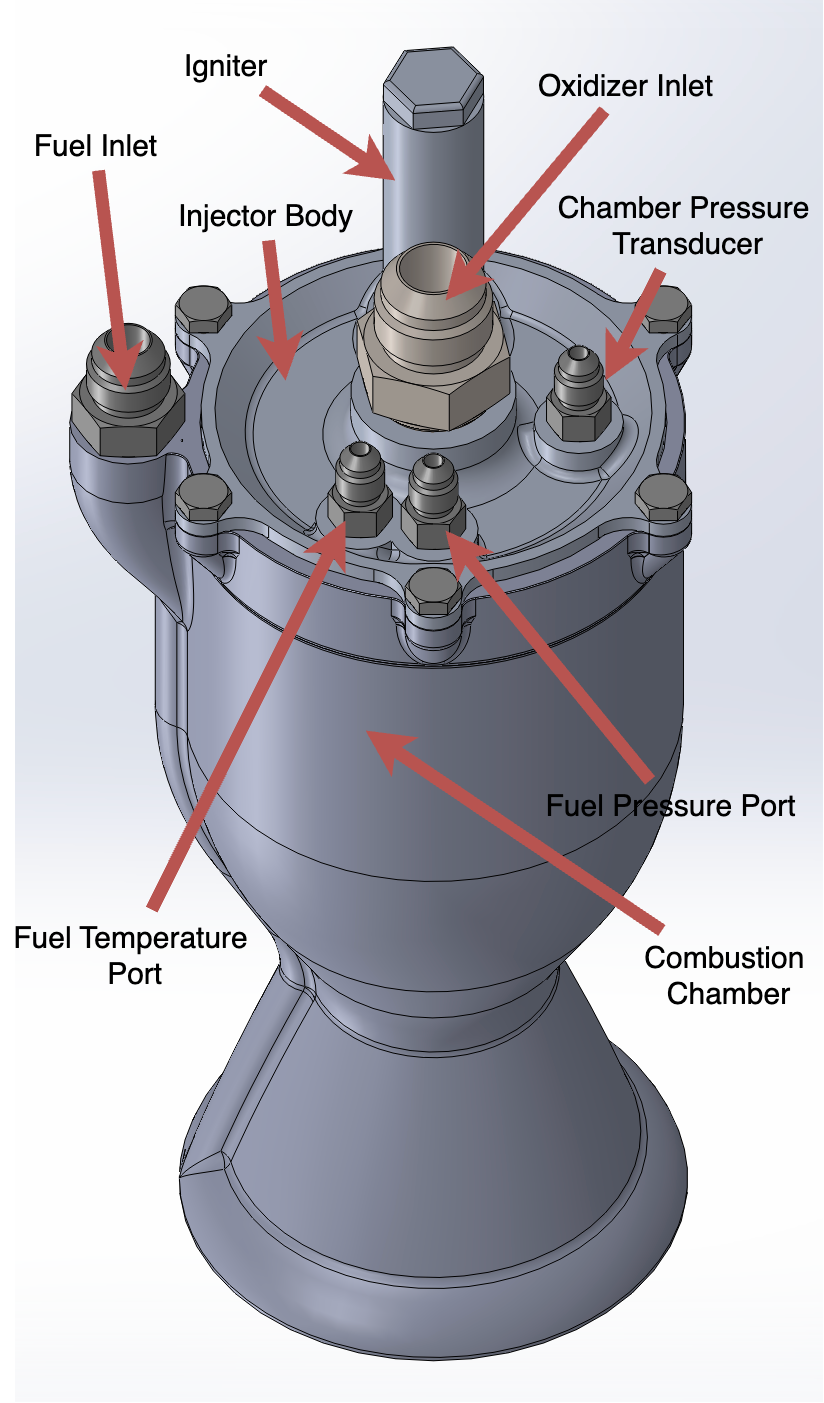
\includegraphics[width=0.8\textwidth]{Images/fullassembly.png}
    \caption{Full assembly view of the 1250 lbf bipropellant rocket engine}
    \label{fig:fullassembly}
\end{figure}

\section{Igniter Design}

\begin{figure}[H]
    \centering
    \includegraphics[width=0.5\textwidth]{Images/IgniterView.png}
    \caption{Igniter assembly view}
    \label{fig:igniter}
\end{figure}

The igniter is a crucial component in the ethanol/nitrous oxide engine, as it initiates combustion and ensures stable ignition of the propellants. Designing the igniter for this engine requires careful consideration to prevent overpressure events, ensure reliable ignition under varying conditions, and integrate with the pintle injector manifold.

\subsection{Ignition Requirements}

For the ethanol/nitrous oxide engine, the igniter must:
\begin{itemize}
    \item Reliably ignite the propellants without causing a hard start or damaging the combustion chamber.
    \item Provide sufficient heat flux to the ethanol and (N$_2$O) spray pattern to ensure rapid and uniform ignition.
    \item Minimize the risk of debris or residue that could disrupt the flow through the injector.
    \item Be compact, reusable (if possible), and compatible with the injector and chamber configuration.
\end{itemize}


\subsection{Solid Motor Cartridge Igniters}

The selected baseline for ignition is a solid motor cartridge igniter, which is available off the shelf as a Quest Q-jet motor and burns independently of the chamber conditions. A solid cartridge igniter simplifies integration and ensures consistent heat flux to the ethanol/nitrous oxide propellants.

\subsubsection{Baseline Design}

The proposed igniter is based on a Quest 18 mm motor, with a burn time of approximately 1.5 seconds \cite{aerotech_motor}. This motor is positioned to fire directly into the pintle injector's spray pattern, providing uniform heating to the propellants as they are atomized.

\textbf{Advantages:}
\begin{itemize}
    \item \textbf{Independent Combustion:} The solid motor burns consistently regardless of chamber pressure or propellant flow conditions, ensuring reliable ignition.
    \item \textbf{No Debris Ejection:} Unlike loose APCP igniters, the cartridge design fully contains the burning propellant, preventing ejection of chunks that could cause a hard start.
    \item \textbf{Ease of Integration:} The solid motor cartridge is compact, easy to install, and fires directly into the pintle spray, ensuring optimal heat transfer.
    \item \textbf{Reduced Maintenance:} Compared to black powder igniters, the APCP-based cartridge produces minimal corrosive residue, reducing wear and tear on the chamber.
\end{itemize}

\textbf{Challenges:}
\begin{itemize}
    \item \textbf{High Heat Flux:} The high-temperature gases produced during ignition could potentially damage chamber walls or the pintle if not carefully controlled.
    \item \textbf{Limited Burn Duration:} The 1.5-second burn time must be sufficient to ignite the ethanol/nitrous propellants; insufficient ignition time could lead to incomplete combustion initiation.
\end{itemize}



\subsection{Advanced Ignition Options: N\textsubscript{2}O Torch Igniter}

An advanced option for ignition is a nitrous oxide (N\textsubscript{2}O) monopropellant torch igniter. This system uses the catalytic decomposition of nitrous oxide to produce high-temperature gases for ignition. While more complex than a solid motor cartridge, this method offers several advantages specific to ethanol/nitrous engines.

\textbf{Advantages:}
\begin{itemize}
    \item \textbf{Clean Combustion:} The catalytic decomposition of N\textsubscript{2}O produces minimal residue, ensuring a clean chamber environment.
    \item \textbf{Chamber Independence:} Like the solid motor, the torch igniter is choked so it operates independently of chamber conditions, providing consistent ignition performance.
    \item \textbf{Heat Control:} By regulating the flow rate of nitrous oxide, the torch igniter can deliver adjustable heat flux tailored to the ignition needs of the engine.
\end{itemize}

\textbf{Challenges:}
\begin{itemize}
    \item \textbf{System Complexity:} The need for a catalytic bed and controlled flow system increases hardware complexity and integration challenges.
    \item \textbf{Development Time:} The N\textsubscript{2}O torch igniter requires further testing to ensure compatibility with the pintle injector and ethanol spray.
\end{itemize}

\subsection{Igniter Placement and Integration}

For both solid motor cartridges and N\textsubscript{2}O torch igniters, the placement within the engine is critical. The igniter is positioned directly adjacent to the pintle injector, ensuring that the igniter flame impinges on the atomized spray pattern. This direct ignition ensures uniform and rapid startup of the engine, and minimises the risk of a hard-start.

\subsection{Comparative Analysis}

\begin{table}[H]
    \centering
    \begin{tabular}{|l|l|l|}
        \hline
        \textbf{Criteria} & \textbf{Solid Motor Cartridge} & \textbf{N\textsubscript{2}O Torch Igniter} \\
        \hline
        Combustion Residue & Minimal & None \\
        \hline
        Ignition Consistency & High & High \\
        \hline
        Complexity & Low & High \\
        \hline
        Adjustability & None (fixed burn) & Adjustable \\
        \hline
        Development Effort & Mature technology & Requires further development \\
        \hline
    \end{tabular}
    \caption{Comparison of Solid Motor and N\textsubscript{2}O Torch Igniters}
    \label{tab:igniter_comparison}
\end{table}



\subsection{Igniter Conclusion}

The baseline igniter for the ethanol/nitrous oxide engine is the solid motor cartridge igniter, specifically the Aerotech Q-Jet 18 mm motor. This choice offers a reliable, low-complexity ignition solution that is compatible with the pintle injector and ensures consistent ignition. 

While the N\textsubscript{2}O monopropellant torch igniter presents an exciting alternative due to its clean combustion and adjustable heat flux, its increased complexity and development effort make it more suitable for future iterations of the engine.


\section{Injector Design: Pintle vs. Showerhead}

The injector is one of the most critical components in liquid rocket engines, responsible for introducing, atomizing, and mixing propellants in the combustion chamber. It determines the combustion efficiency, combustion stability, and thermal profile within the combustion chamber, making its design a critical aspect of engine performance. Two primary injector designs are considered in this trade study: the \textbf{pintle injector} and the \textbf{showerhead injector}. This section explores the operating principles, advantages, limitations, and suitability of each design for various rocket engine applications.


\subsection{Pintle Injector}

\subsubsection{Design and Operating Principles}

The pintle injector consists of a central pintle element, through which one propellant—typically the oxidizer—flows axially. The second propellant—commonly the fuel—is introduced radially or tangentially through an annular slot or discrete orifices around the pintle. As the two propellants impinge on eachother, they generate a spray cone and a turbulent recirculation zone downstream of the pintle tip, leading to highly efficient mixing and combustion.

In more advanced designs, the pintle injector's geometry allows precise control over the mixing of the propellants by adjusting the pintle's axial position. This feature, combined with its inherent simplicity, makes it a preferred design for engines requiring high stability and variable thrust.

\textbf{Historical Use:} The pintle injector gained prominence in the Apollo Lunar Module Descent Engine (LMDE). The injector's ability to throttle smoothly and deliver stable combustion under varying conditions was pivotal for the success of precision lunar landings. The same fundamental design has been employed in numerous other rocket engines, including the SpaceX Merlin engines.



\subsubsection{Advantages}

\begin{itemize}
    \item \textbf{Superior Combustion Stability:} The pintle's self-contained recirculation zone promotes effective mixing and mitigates acoustic and thermal instabilities, making it inherently more stable than multi-element designs.
    \item \textbf{Exceptional Throttling Capability:} Pintle injectors can achieve deep throttling ratios (up to 10:1 or greater) with minimal performance degradation, making them suitable for reusable and landing systems.
    \item \textbf{Manufacturability and Cost-Effectiveness:} Compared to the showerhead injector, the pintle's simpler geometry reduces manufacturing complexity, especially for small-to-medium thrust engines.
    \item \textbf{Proven Heritage:} Decades of successful operation in space missions demonstrate the reliability and robustness of the pintle injector design.
    \item \textbf{Adaptability to Diverse Propellants:} Pintle injectors have been demonstrated with various combinations of cryogenic, storable, and hypergolic propellants.
\end{itemize}



\subsubsection{Challenges and Limitations}

\begin{itemize}
    \item \textbf{Flow Asymmetry:} The pintle injector’s flow dynamics can lead to asymmetric combustion and uneven heat flux distributions on the chamber walls, which may lead to chamber failure.
    \item \textbf{Thermal Stress and Erosion:} The high temperatures and high oxidizer environment near the pintle tip can increase erosion rates and thermal stress, potentially shortening component life.
\end{itemize}


\subsection{Showerhead Injector}

\subsubsection{Design and Operating Principles}

The showerhead injector consists of a faceplate with an array of small orifices through which propellants are injected into the combustion chamber. Each orifice produces its own spray plume, resulting in multiple discrete mixing zones. The showerhead design focuses on distributing propellants uniformly across the combustion chamber to achieve even combustion and thermal loading.

This injector design has been widely used in high-thrust engines, such as the RS-25 (Space Shuttle Main Engine) and RL10, where precise control of propellant distribution is critical.


\subsubsection{Advantages}

\begin{itemize}
    \item \textbf{Uniform Propellant Distribution:} The distributed flow from multiple orifices ensures even heat flux and reduces the risk of localized hotspots, promoting longer chamber life.
    \item \textbf{Scalability:} The modular nature of the design allows for easy scaling by increasing or decreasing the number and size of orifices.
    \item \textbf{Thermal Management:} Uniform combustion mitigates thermal gradients, reducing thermal stress on chamber walls.
    \item \textbf{Performance at High Thrust Levels:} The showerhead design excels in engines requiring extremely high thrust outputs, as it evenly distributes large mass flow rates.
\end{itemize}



\subsubsection{Challenges and Limitations}

\begin{itemize}
    \item \textbf{Susceptibility to Combustion Instabilities:} The absence of natural recirculation zones increases the likelihood of acoustic and thermal instabilities.
    \item \textbf{Throttling Limitations:} Fixed orifice geometries limit the showerhead's ability to throttle effectively without significant modifications to the flow control systems.
    \item \textbf{Manufacturing Complexity:} Precision machining of multiple orifices adds cost and complexity, particularly for engines requiring highly uniform flow.
    \item \textbf{Non-Optimal Mixing:} Mixing efficiency depends heavily on the orifice layout and may require extensive testing to optimize. The showerhead is not optimal for liquid-liquid bipropellant engines due to poor atomization. 
\end{itemize}

\subsection{Comparative Analysis}
\begin{table}[H]
    \centering
    \begin{tabularx}{\textwidth}{|X|X|X|}
        \hline
        \textbf{Criteria} & \textbf{Pintle Injector} & \textbf{Showerhead Injector} \\
        \hline
        Combustion Stability & High; robust against instabilities & Moderate; prone to instabilities \\
        \hline
        Throttling Capability & Deep throttling (up to 10:1) & Limited; fixed orifice geometry \\
        \hline
        Mixing Efficiency & Excellent; natural recirculation & Moderate; depends on orifice layout \\
        \hline
        Heat Flux Distribution & Asymmetric; requires cooling & Uniform; manageable cooling demands \\
        \hline
        Manufacturability & Relatively simple & Complex; precision machining required \\
        \hline
        Scalability & Suitable for small-to-medium thrust engines & Ideal for high-thrust applications \\
        \hline
    \end{tabularx}
    \caption{Comparison of Pintle and Showerhead Injectors}
    \label{tab:injector_comparison}
\end{table}



\subsection{Injector Pintle Design}

\begin{figure}[H]
    \centering
    \includegraphics[width=0.5\textwidth]{Images/PintleInjectorView.png}
    \caption{View of the pintle injector and Injector Manifold}
    \label{fig:pintle_injector}
\end{figure}

The injector system consists of two primary components: the \textbf{pintle insert} and the \textbf{pintle annulus}. These components form the basis of the fuel-oxidizer delivery system. Fuel is injected axially through the annulus, while oxidizer (nitrous oxide) is injected radially through 44 orifices drilled into the pintle tip. The oxidizer and fuel impinge at the interface, creating a high-shear, turbulent mixing zone, which causes effective atomization and mixing of the propellants.

\subsubsection{Pintle Alignment}

Maintaining precise concentric alignment between the pintle insert and the outer annulus is essential for ensuring symmetric propellant flow and preventing asymmetric combustion, which could damage the combustion chamber walls. Any deviation in alignment can cause uneven oxidizer-fuel mixing, leading to incomplete combustion, reduced specific impulse (I$_{sp}$), and even combustion instabilities such as chugging or hard starts. 

The mechanical interface between the pintle and the annulus is designed with tight tolerances, ensuring minimal misalignment. The orifices characteristics for Nitrous injection were determined with empirical data from the Waxman paper \textit{"An Investigation of Injectors for Use with High Vapor Pressure Propellants with Applications to Hybrid Rockets"}
\cite{wax}

\subsubsection{Fuel and Oxidizer Flow Characteristics}

\paragraph{Oxidizer Flow Regulation:}

According to the findings in Benjamin Waxman’s paper \emph{An Investigation of Injectors for Use with High Vapor Pressure Propellants with Applications to Hybrid Rockets}, nitrous oxide injection operates in a \textbf{near-critical flow} regime rather than a fully choked flow condition due to the thermodynamic properties of nitrous oxide. While traditional gases can easily achieve fully choked flow when the pressure ratio ($P_{\text{upstream}} / P_{\text{downstream}}$) exceeds the critical value of approximately 1.89 for diatomic gases, liquid nitrous oxide's high vapor pressure and compressibility introduce additional complexity.

The Waxman study demonstrated that nitrous oxide experiences a \emph{pseudo-choked} condition near the orifice exit, where the flow rate stabilizes but may still respond to minor downstream pressure fluctuations. This occurs because nitrous oxide behaves as a saturated vapor-liquid mixture at typical injector inlet conditions, causing a flow regime shift depending on injector pressure and temperature.

Despite this complexity, the mass flow rate is still largely controlled by the upstream pressure, minimizing the effect of downstream pressure oscillations when the upstream-to-downstream pressure ratio is sufficiently high. This quasi-stable condition ensures relatively consistent oxidizer flow, making nitrous oxide viable for pressure-fed bipropellant engines with carefully designed injector geometries. In the engine's pintle injector, the orifice dimensions are selected based on empirical flow data from the Waxman paper, ensuring predictable mass flow behavior under operating conditions.



\subsubsection{Orifice Design and Validation}

The pintle orifice design was selected based on experimental data from the Waxman paper, which provided validated flow characteristics for an orifice with a diameter of 1.5 mm and a length of 3.2 mm. This specific orifice size was chosen due to its well-characterized mass flow performance, enabling accurate prediction of the oxidizer flow rate under various pressure conditions.

\begin{figure}[H]
    \centering
    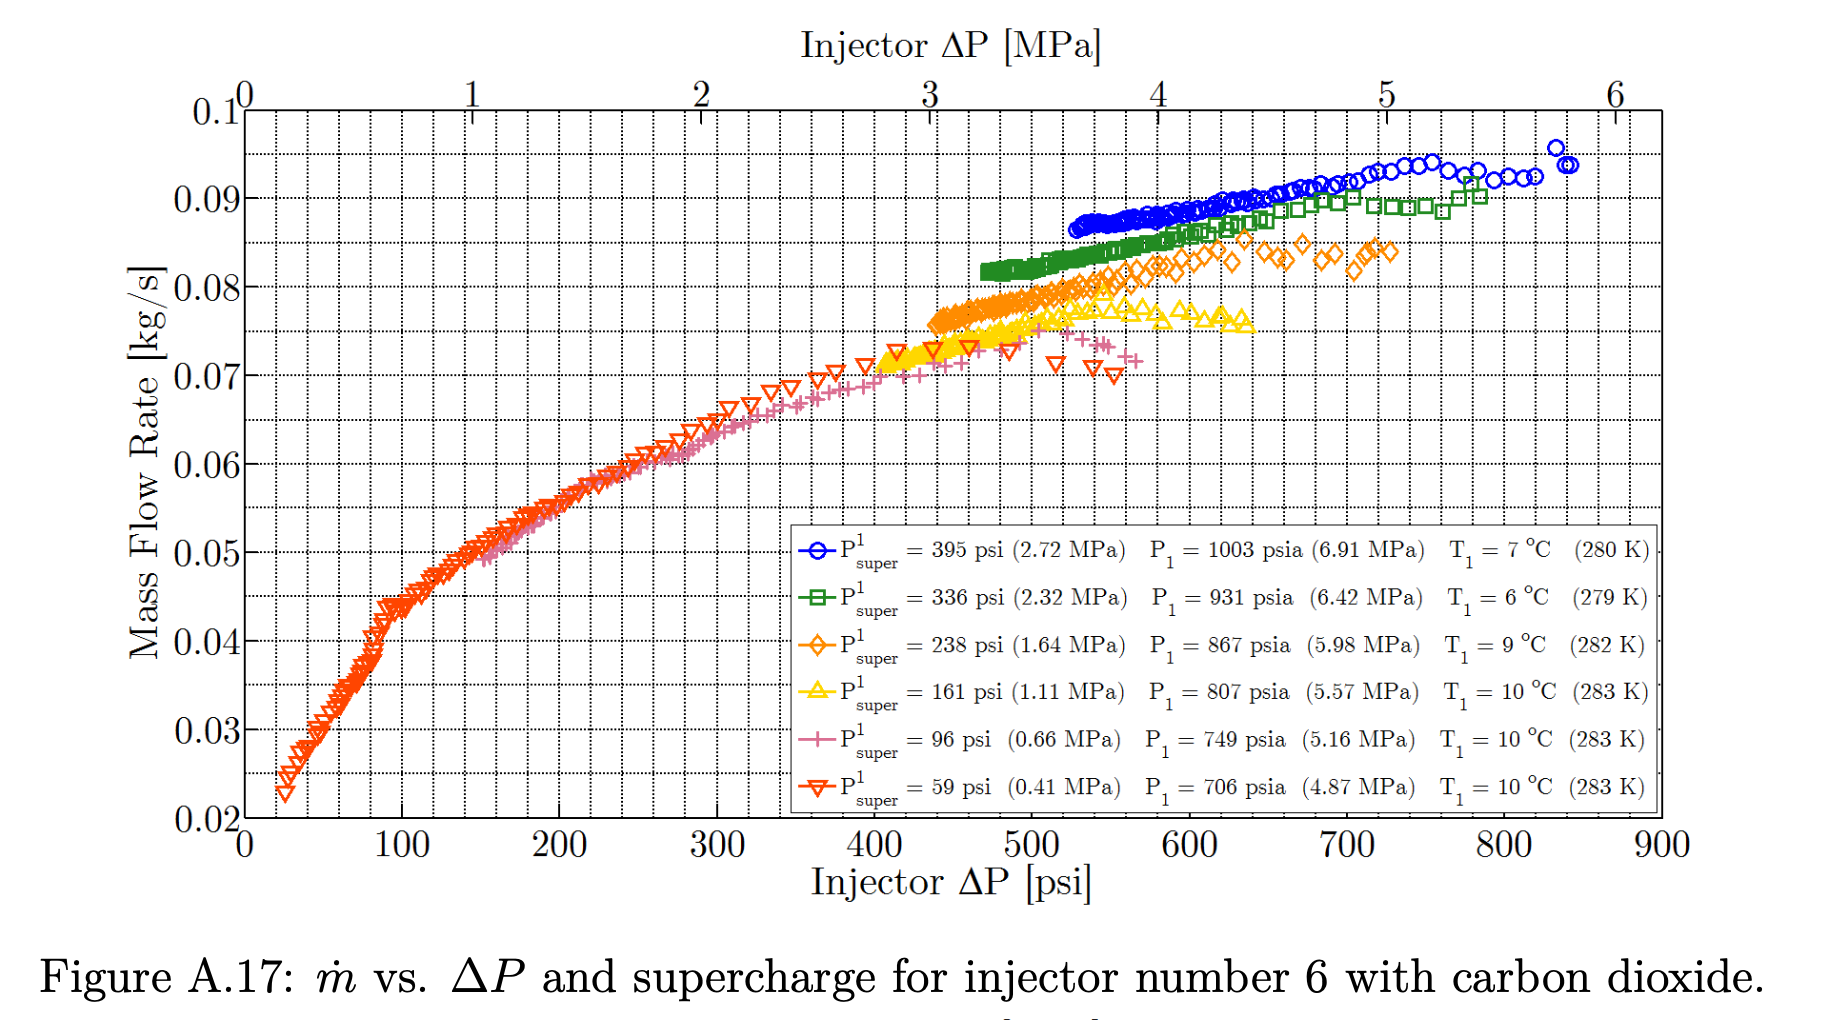
\includegraphics[width=1.0\linewidth]{waxmanorifice6.png}
    \caption{Waxman 1.5mm diameter, 3.2mm length orifice data}
    \label{fig:wax_orifice}
\end{figure}


The Imperial College London (ICL) team reported using a similar pintle design, achieving a pressure drop of 4.1 bar (59.47 psi) across 48 orifices, resulting in a total oxidizer mass flow rate of 1.55 kg/s. This corresponds to a flow rate of approximately 0.0322 kg/s per orifice, matching Waxman’s experimental results for CO\textsubscript{2} as an analog for N\textsubscript{2}O.

\paragraph{Mass Flow Rate Calculation:}
Based on the desired oxidizer mass flow rate of 2.5788 kg/s for the engine, the required number of orifices was calculated as follows:

\begin{equation}
n = \frac{\dot{m}_{ox}}{\dot{m}_{orifice}} = \frac{2.5788}{0.06} \approx 43
\end{equation}

Given that three rows of orifices were selected, each row contains approximately 14 orifices:

\begin{equation}
n_{\text{row}} = \frac{43}{3} \approx 14.33
\end{equation}


\subsubsection{Injection Pressure and Stiffness}

The injector's effect on combustion stability is heavily influenced by its \textbf{injection stiffness}, defined as:

\begin{equation}
\text{Stiffness} = \frac{P_{\text{feed}} - P_{\text{chamber}}}{P_{\text{chamber}}}
\end{equation}

Injection stiffness must be maintained at or above 30\% to remain insensitive to combustion chamber pressure fluctuations caused by combustion instabilities. A stiffness of 60\% or higher is recommended to ensure stable oxidizer and fuel delivery even under off-nominal conditions.
\begin{figure}[H]
    \centering
    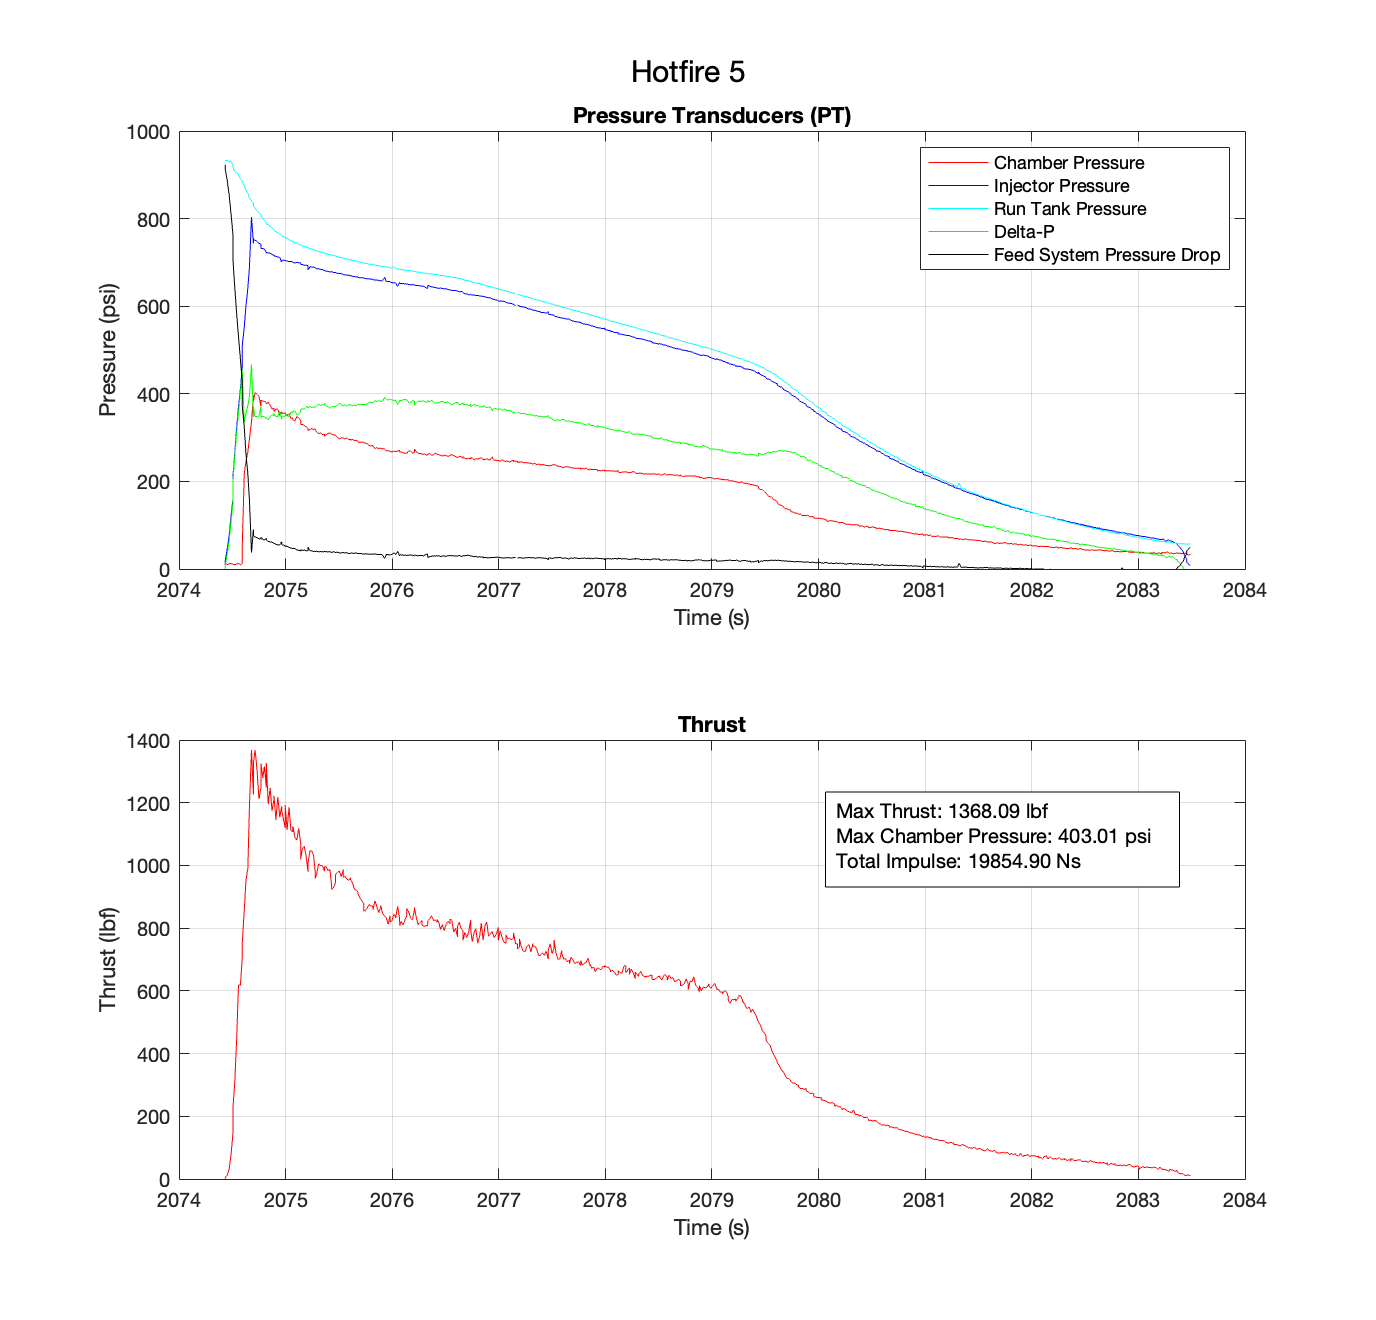
\includegraphics[width=1.0\linewidth]{hybriddata.png}
    \caption{Volta III Delta-P Data}
    \label{fig:enter-label}
\end{figure}
Based on CRT hybrid engine data from the Volta III engine, a pressure delta ($\Delta P$) of approximately 390 psi was assumed. This value aligns with previous injector configurations and provides sufficient stiffness to maintain critical flow conditions in the oxidizer orifices 
\cite{wax}










\subsection{Injector CAD Images}
\begin{figure}[H]
    \centering
    \includegraphics[width=0.5\textwidth]{Images/Pintle.png}
    \caption{Injector pintle design used for regulating oxidizer flow into the combustion chamber. The geometry ensures optimal mixing of the oxidizer and fuel for efficient combustion.}
    \label{fig:pintle}
\end{figure}





\begin{figure}[H]
    \centering
    \includegraphics[width=0.8\textwidth]{Images/ManifoldCrossSection.png}
    \caption{Cross-section of the injector manifold showing the internal flow paths for oxidizer distribution. The design ensures uniform flow to the injector pintle.}
    \label{fig:manifold_crosssection}
\end{figure}
\begin{figure}[H]
    \centering
    \includegraphics[width=0.8\textwidth]{Images/InjectorManifoldIsoView.png}
    \caption{Isometric view of the injector manifold highlighting its external features and mounting points.}
    \label{fig:manifold_isoview}
\end{figure}

\begin{figure}[H]
    \centering
    \includegraphics[width=0.8\textwidth]{Images/InjectorManifoldSideView.png}
    \caption{Side view of the injector manifold showing the integration with the combustion chamber assembly.}
    \label{fig:manifold_sideview}
\end{figure}


\begin{figure}[H]
    \centering
    \includegraphics[width=0.8\textwidth]{Images/AnotherInjectorView.png}
    \caption{Injector assembly featuring all integrated components. This view shows the assembled state for proper alignment and sealing.}
    \label{fig:injector_assembly}
\end{figure}




\begin{figure}[H]
    \centering
    \includegraphics[width=0.8\textwidth]{Images/TopView.png}
    \caption{Top-down view of the combustion chamber and injector assembly. Demonstrates the alignment and layout of the injector with the chamber.}
    \label{fig:topview}
\end{figure}



\section{Fuel Selection Trade Study}

\subsection{Ethanol vs. IPA vs. Kerosene}
Ethanol was selected due to its lower viscosity and cleaner combustion compared to kerosene. IPA was less desirable due to higher cost and similar properties.

\subsection{Oxidizer: N$_2$O}
Nitrous oxide was chosen due to our extensive experience working with this oxidizer. It is also not a cryogenic so this makes procurement much easier than LOX for example.

\section{Motor Calculations} 



\subsection{O/F and Chamber Pressure Selection}
To determine the most optimal O/F ratio for this application I plotted specific impulse vs O/F ratio for a variety of chamber pressures. I selected a chamber pressure of 350 PSI and an O/F of 3.8 because there was little ISP to be gained by increasing these parameters, and increasing O/F leads to thermal issues. Increasing chamber pressure is possible but does add risk for marginal benefit in this situation. 
\begin{figure}[H]
    \centering
    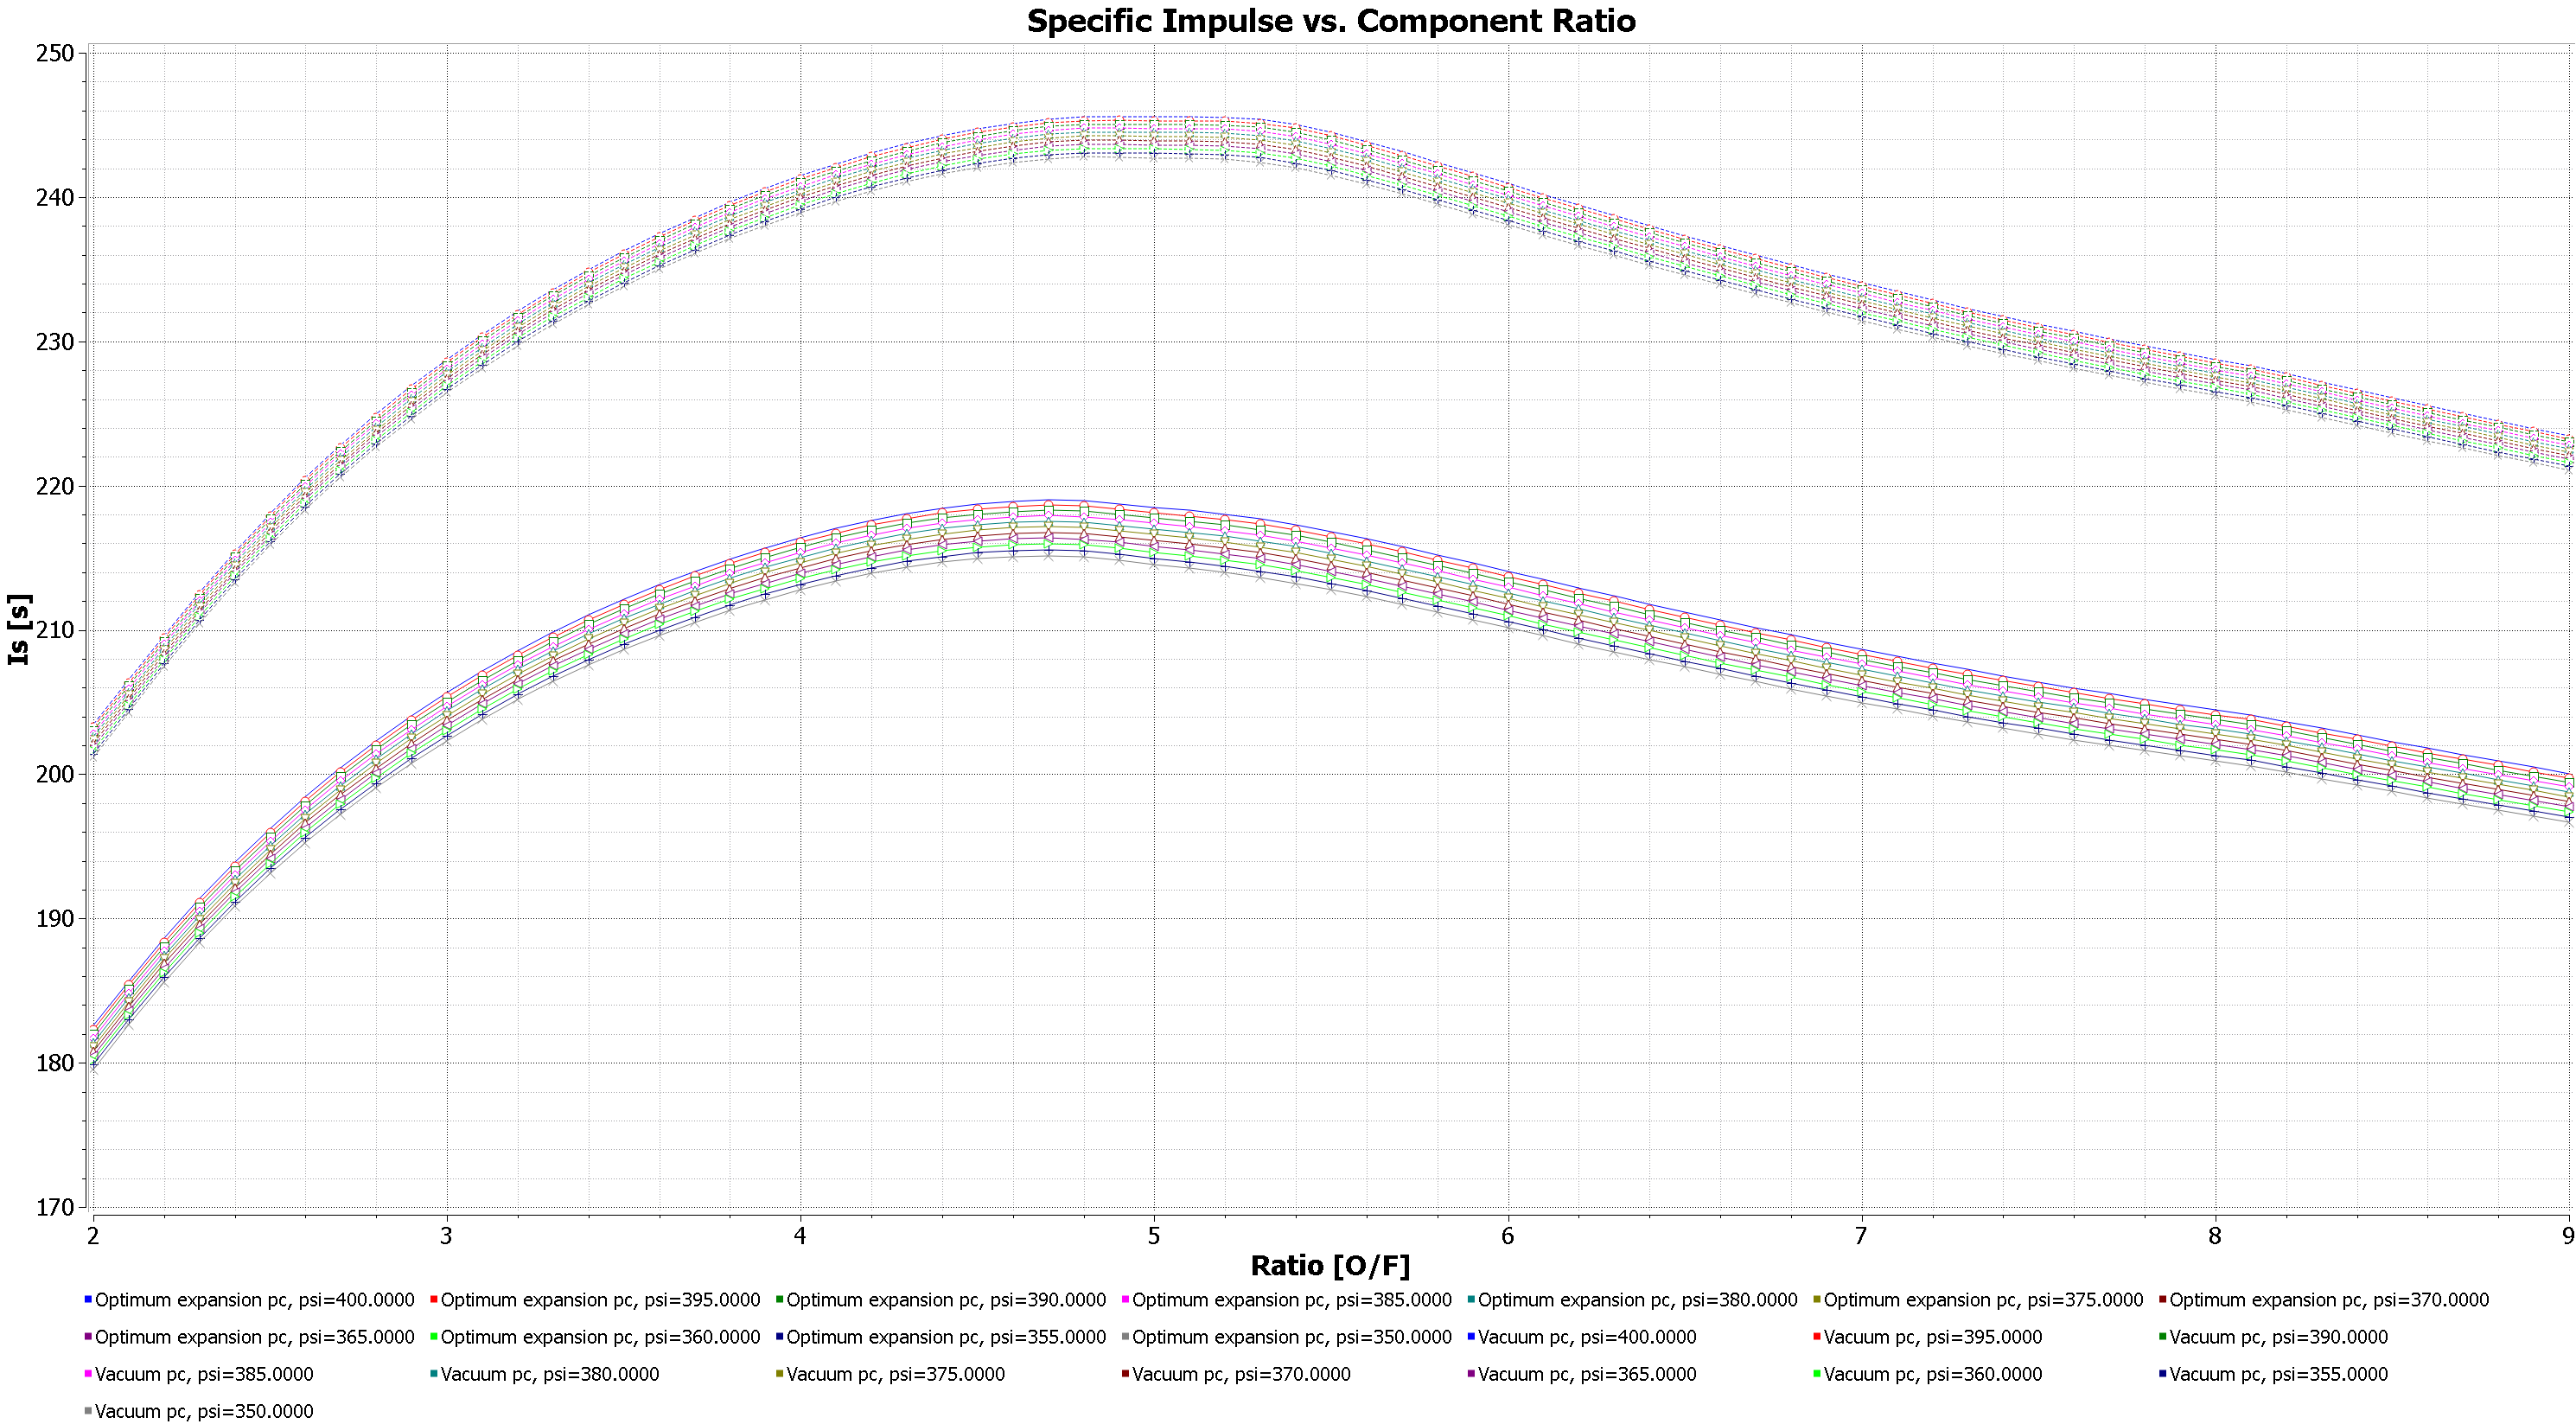
\includegraphics[width=1.0\linewidth]{Images/ispvscomponentratio.png}
    \caption{ISP vs OF ratio}
    \label{fig:enter-label}
\end{figure}

\subsection{Chamber Sizing}
To size the chamber
\begin{figure}[H]
    \centering
    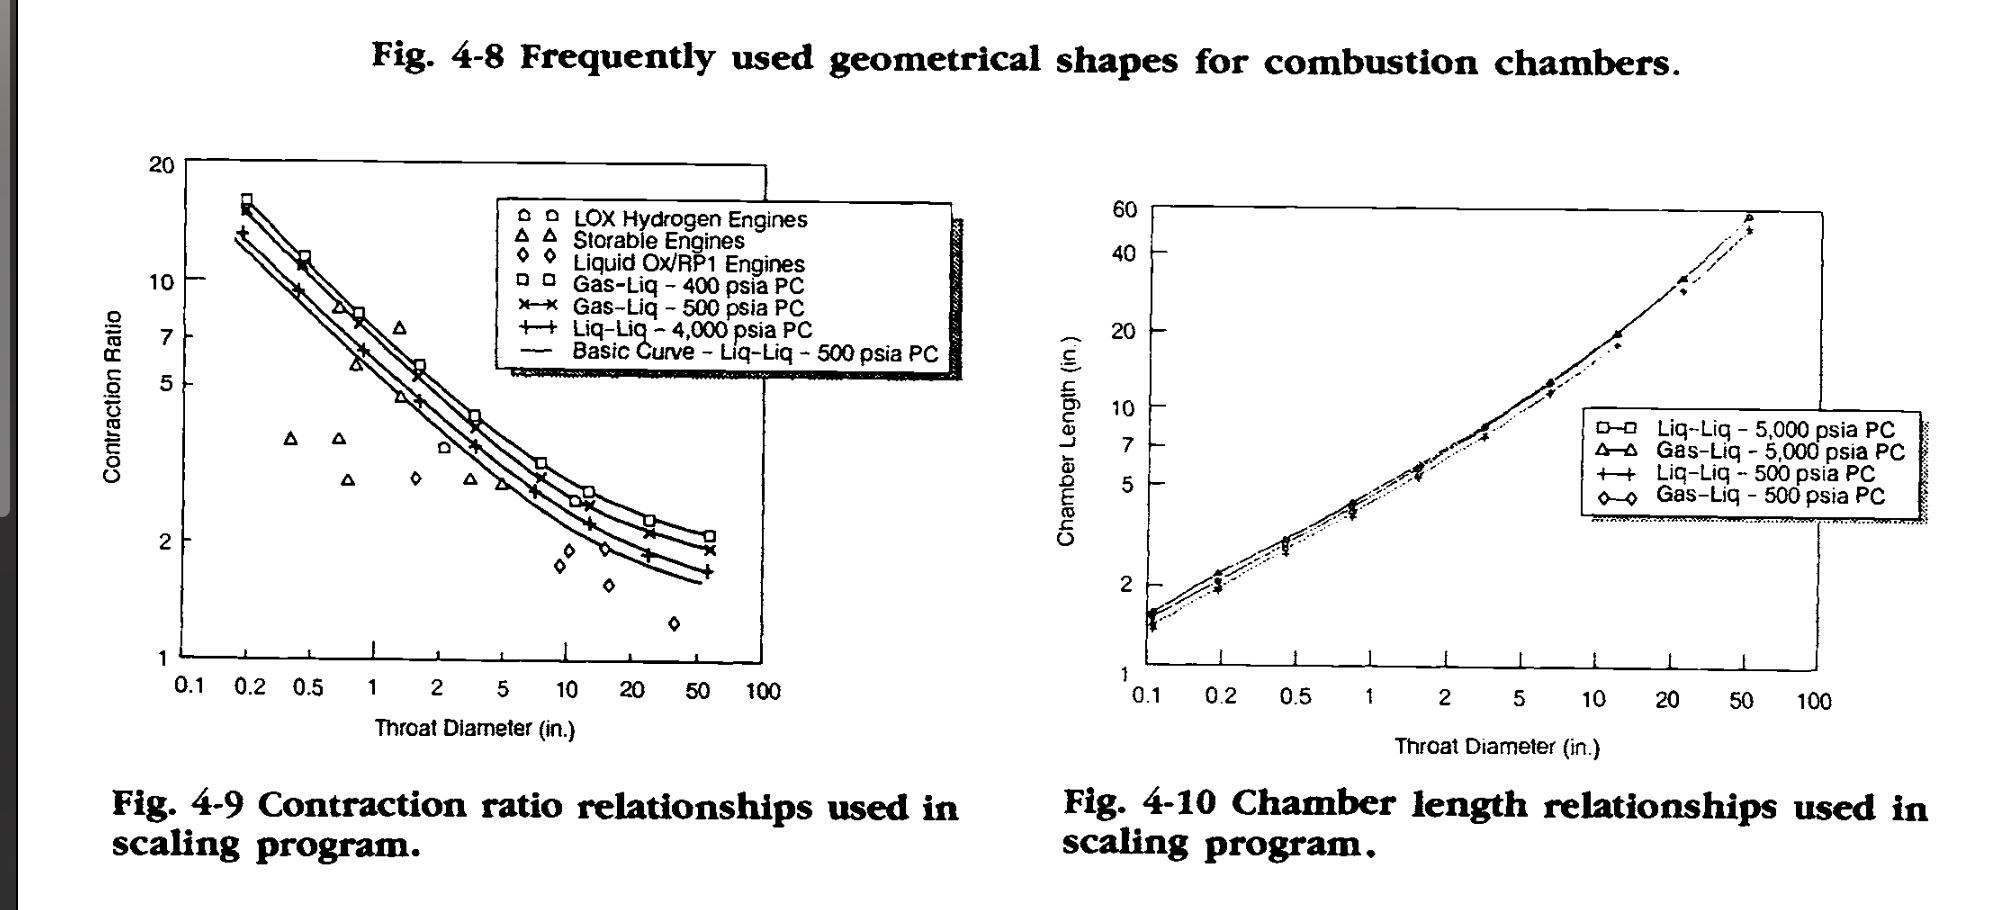
\includegraphics[width=0.75\linewidth]{Images/lstar.png}
    \caption{Characteristic Sizes}
    \label{fig:enter-label}
\end{figure}


\begin{figure}[H]
    \centering
    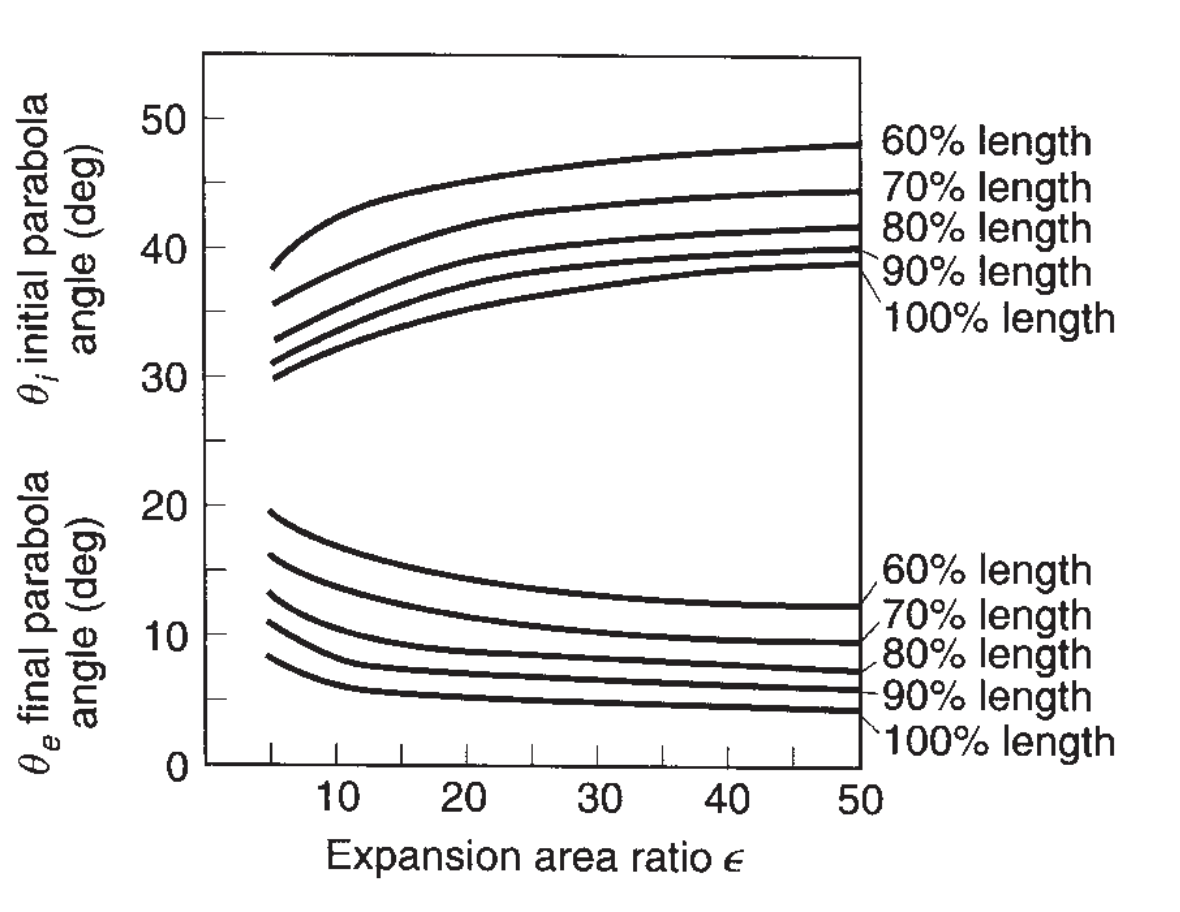
\includegraphics[width=0.75\linewidth]{nozzleshape.png}
    \caption{Bell Nozzle Parabola Angles}
    \label{fig:enter-label}
\end{figure}
     \begin{enumerate}

     
\item Use the relationship between throat diameter and contraction ratio to determine the contraction ratio based on the most relevant curve which happens to be the liq-liq curve at 500 psia (left graph).
  
\item Again map the throat diameter to find the corresponding characteristic chamber length (L*) within the 250mm limitation of the 3D printer bed.   


\end{enumerate}


Using RPA, the following parameters were inputted:
\begin{itemize}
    \item Chamber pressure: 350 psi
    \item Desired thrust: 1250lbf
    \item Fuel mixture: 80:20 Ethanol to water ratio
    \item Oxidizer: N2O 
\end{itemize}
\section{Engine Parameters}



\subsection{Combustion Chamber Geometry}
\begin{figure}[H]
    \centering
    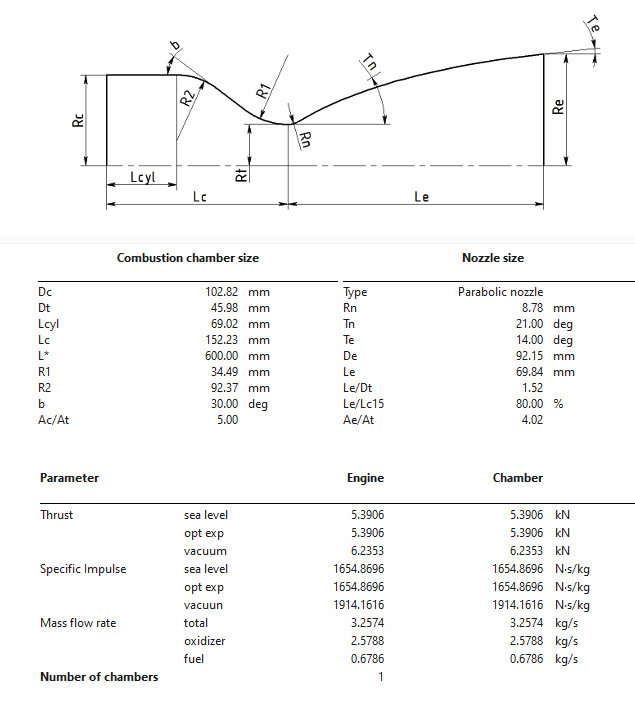
\includegraphics[width=0.75\linewidth]{Images/motordata_final.png}
    \caption{Chamber Parameters}
    \label{fig:enter-label}
\end{figure}

\begin{table}[H]
    \centering
    \begin{tabular}{|l|l|l|}
        \hline
        \textbf{Parameter} & \textbf{Symbol} & \textbf{Value} \\ \hline
        Combustion chamber diameter & \(D_c\) & \SI{102.82}{\milli\meter} \\ \hline
        Throat diameter & \(D_t\) & \SI{45.98}{\milli\meter} \\ \hline
        Cylindrical section length & \(L_{\text{cyl}}\) & \SI{69.02}{\milli\meter} \\ \hline
        Combustion chamber length & \(L_c\) & \SI{152.23}{\milli\meter} \\ \hline
        Characteristic length & \(L^*\) & \SI{600}{\milli\meter} \\ \hline
        Radius of curvature at inlet & \(R_1\) & \SI{34.49}{\milli\meter} \\ \hline
        Radius of curvature at outlet & \(R_2\) & \SI{92.37}{\milli\meter} \\ \hline
        Convergence half-angle & \(b\) & \SI{30}{\degree} \\ \hline
        Area contraction ratio & \(A_c/A_t\) & 5.00 \\ \hline
    \end{tabular}
    \caption{Combustion Chamber Geometry}
\end{table}

\begin{table}[H]
    \centering
    \begin{tabular}{|l|l|l|}
        \hline
        \textbf{Parameter} & \textbf{Symbol} & \textbf{Value} \\ \hline
        Nozzle type & -- & Parabolic nozzle \\ \hline
        Nozzle radius of curvature & \(R_n\) & \SI{8.78}{\milli\meter} \\ \hline
        Throat angle & \(T_n\) & \SI{21.00}{\degree} \\ \hline
        Exit angle & \(T_e\) & \SI{14.00}{\degree} \\ \hline
        Exit diameter & \(D_e\) & \SI{92.15}{\milli\meter} \\ \hline
        Nozzle length & \(L_e\) & \SI{69.84}{\milli\meter} \\ \hline
        Exit-to-throat area ratio & \(A_e/A_t\) & 4.02 \\ \hline
    \end{tabular}
    \caption{Nozzle Geometry}
\end{table}

\subsection{Performance Parameters}
\begin{table}[H]
    \centering
    \begin{tabular}{|l|l|l|}
        \hline
        \textbf{Parameter} & \textbf{Condition} & \textbf{Value} \\ \hline
        Thrust & Sea level & \SI{5.3906}{\kilo\newton} \\ \hline
        Thrust & Vacuum & \SI{6.2353}{\kilo\newton} \\ \hline
        Specific impulse & Sea level & \SI{168.6}{\second} \\ \hline
        Specific impulse & Vacuum & \SI{195.1}{\second} \\ \hline
        Mass flow rate & Total & \SI{3.2574}{\kilogram\per\second} \\ \hline
        Mass flow rate & Oxidizer & \SI{2.5788}{\kilogram\per\second} \\ \hline
        Mass flow rate & Fuel & \SI{0.6786}{\kilogram\per\second} \\ \hline
        Number of combustion chambers & -- & 1 \\ \hline
    \end{tabular}
    \caption{Performance Parameters}
\end{table}





\section{Thermal Analysis}
The thermal analysis is likely the most difficult part of designing a rocket engine. Staying below a maximum wall temperature of 500k for the aluminum engine took many iterations. RPA solves the heat transfer equations based on the input parameters of film cooling and regenerative cooling channels. Levlev and Bartz combined heat transfer calculations were implemented in RPA.
Initially, the wall temperature was too high, so water was added to the fuel up to 20 percent, which increased regenerative cooling mass flow rate and also slightly lowered combustion temperatures. 
Aluminum ended up being the optimal material based on yield strength at wall temperature, and based on widespread availability.
Copper offered some marginal benefits which could possibly have been optimized further but the fact that it is less available to 3D print is a large disadvantage. 



Inconel 718 was initially selected due to its exceptional high-temperature strength, corrosion resistance, and widespread use in aerospace applications. However, several challenges emerged during the design process, ultimately leading to the exclusion of Inconel in favor of aluminum.

The first thermal analysis used 100\% ethanol as the fuel, relying solely on regenerative cooling. Due to Inconel’s low thermal conductivity of approximately \SI{11.4}{\watt\per\meter\per\kelvin}, the heat transfer from the chamber walls to the coolant was insufficient. This resulted in excessively high wall temperatures, exceeding \SI{1000}{\kelvin}.

To mitigate this, film cooling was added by introducing ethanol along the chamber walls through dedicated orifices, however it required significantly more film cooling mass flux than aluminum. 

Inconel’s thermal properties required ultra-thin chamber walls to facilitate regenerative cooling effectively. This posed significant manufacturing challenges because printing Inconel with thin walls is prone to defects such as warping and cracking due to the high residual stresses induced during metal 3D printing. Additionally, Inconel’s extreme hardness and tendency to destroy tools would make post-processing and machining time-consuming and expensive, reducing its feasibility.



After considering thermal analysis and manufacturability constraints Inconel was ultimately replaced with aluminum AlSi10Mg, which offered better thermal conductivity (\SI{150}{\watt\per\meter\per\kelvin}) and was more optimal for regenerative cooling. Its lower melting point was offset by optimized film and regenerative cooling designs, allowing for operation while staying below the \SI{500}{\kelvin} maximum wall temperature. While copper provided slightly better thermal performance, its limited availability for 3D printing made aluminum the most practical and effective material choice.

\begin{table}[h!]
    \centering
    \begin{tabular}{|l|l|}
        \hline
        \textbf{Parameter} & \textbf{Value} \\ \hline
        Maximum heat flux at the throat & \SI{246.80}{\kilo\watt\per\meter\squared} \\ \hline
        Maximum wall temperature (gas side) & \SI{467.98}{\kelvin} \\ \hline
        Maximum wall temperature (coolant side) & \SI{452.74}{\kelvin} \\ \hline
        Maximum coolant temperature & \SI{353.00}{\kelvin} \\ \hline
        Average coolant velocity & \SI{6.16}{\meter\per\second} \\ \hline
        Average coolant density & \SI{800.92}{\kilogram\per\meter\cubed} \\ \hline
    \end{tabular}
    \caption{Aluminum Engine Thermal Analysis}
\end{table}

\subsection{Material Specifications}

\begin{table}[H]
    \centering
    \begin{tabular}{|l|l|l|l|}
        \hline
        \textbf{Property} & \textbf{AlSi10Mg (EOS)} & \textbf{Inconel 718 (EOS)} & \textbf{CuZnZn (EOS)} \\ \hline
        Material Type & Aluminum Alloy & Nickel Alloy & Copper Alloy \\ \hline
        Yield Strength at 250°C & \SI{125}{\mega\pascal} & \SI{1030}{\mega\pascal} & \SI{150}{\mega\pascal} \\ \hline
        Ultimate Tensile Strength & \SI{230}{\mega\pascal} & \SI{1240}{\mega\pascal} & \SI{315}{\mega\pascal} \\ \hline
        Density & \SI{2700}{\kilo\gram\per\meter^3} & \SI{8190}{\kilo\gram\per\meter^3} & \SI{8500}{\kilo\gram\per\meter^3} \\ \hline
        Thermal Conductivity at 250°C & \SI{150}{\watt\per\meter\per\kelvin} & \SI{11.4}{\watt\per\meter\per\kelvin} & \SI{320}{\watt\per\meter\per\kelvin} \\ \hline
        Melting Point & \SI{570}{\celsius} & \SI{1350}{\celsius} & \SI{1083}{\celsius} \\ \hline
    \end{tabular}
    \caption{Material Specifications for EOS 3D-Printed Alloys}
    \label{tab:material_specs}
\end{table}
\begin{figure}[H]
    \centering
    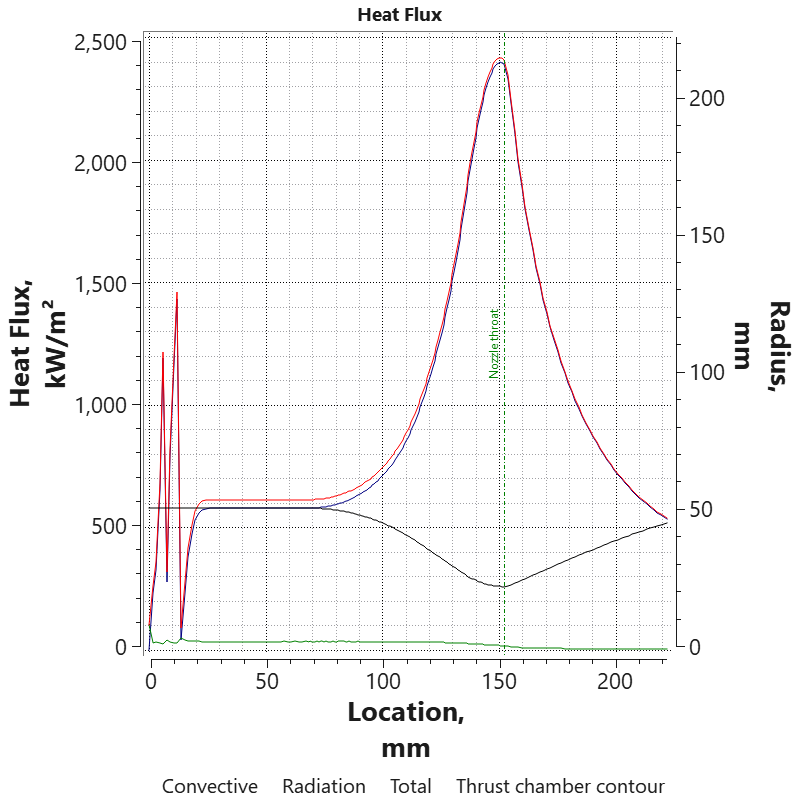
\includegraphics[width=0.75\linewidth]{Images/aluminiumfinalheatflux.png}
    \caption{Aluminum Engine Heat Flux along Profile}
    \label{fig:aluminum_heat_flux}
\end{figure}


\begin{figure}[H]
    \centering
    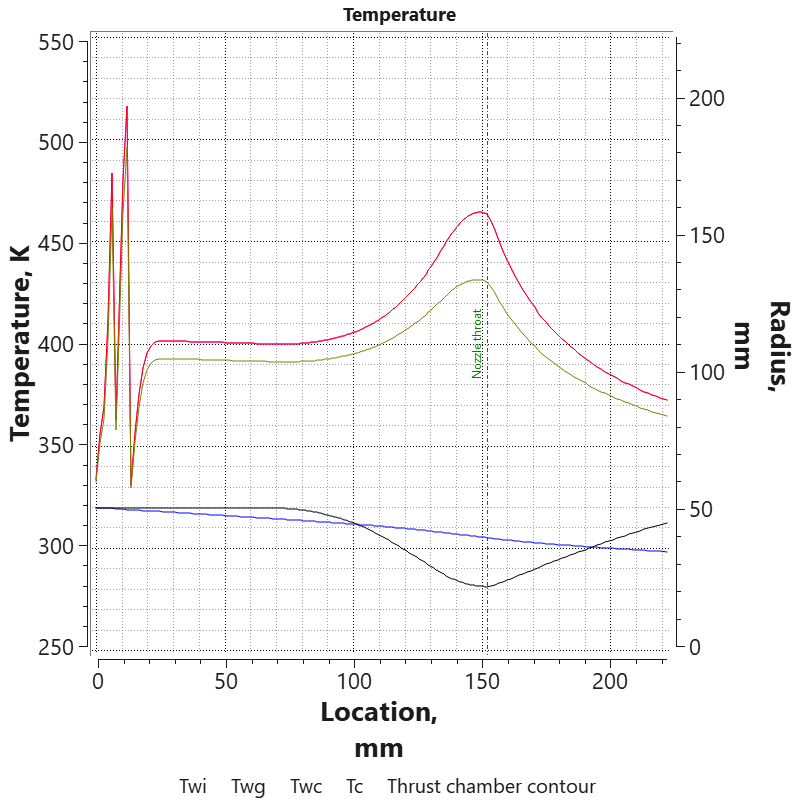
\includegraphics[width=\linewidth]{Images/tempfinal_AL_53.png}
    \caption{Aluminum Engine Temperature Profile under Nominal Operation}
    \label{fig:aluminum_temp_profile}
\end{figure}

\begin{figure}
    \centering
    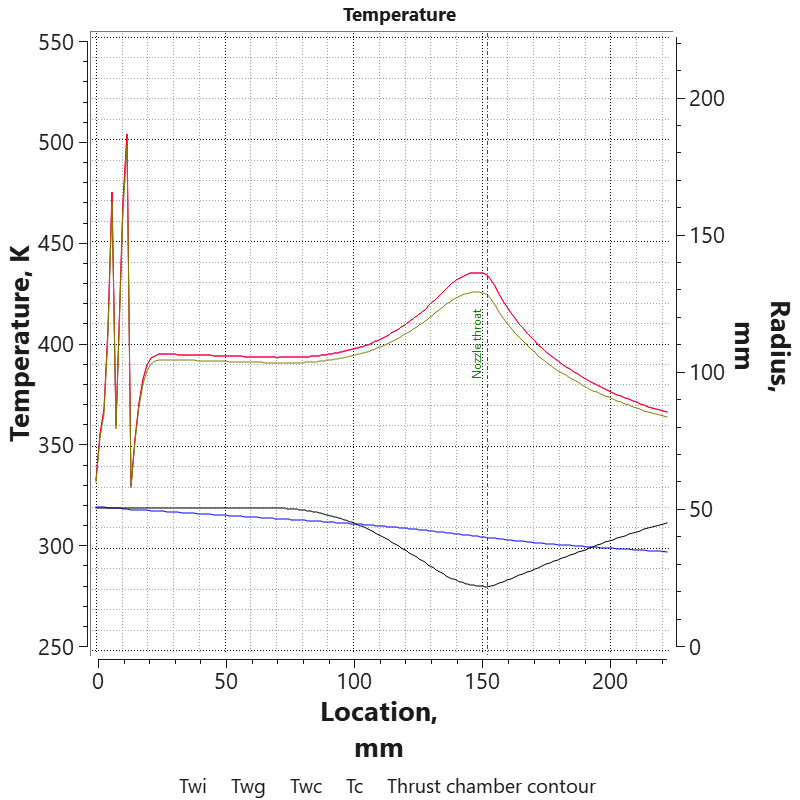
\includegraphics[width=0.75\linewidth]{tempfinal_CUzn_5film.png}
    \caption{Copper Engine Temperature Profile under Nominal Operation}
    \label{fig:enter-label}
\end{figure}
\begin{figure}[H]
    \centering
    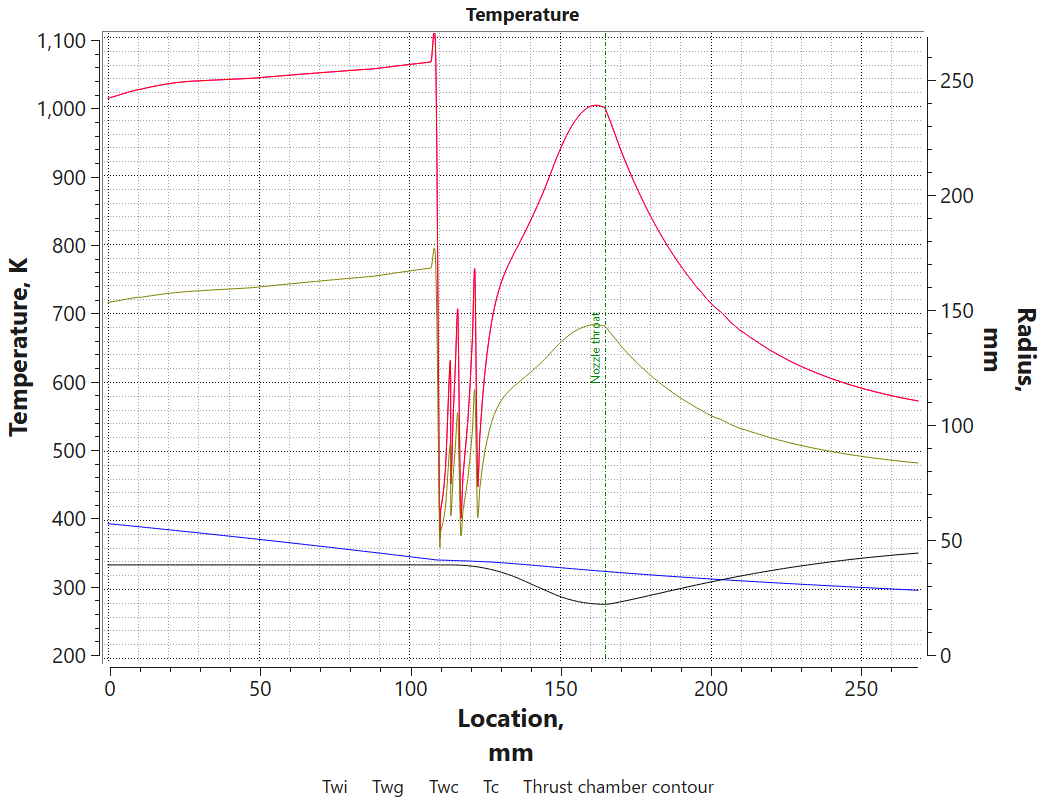
\includegraphics[width=0.75\linewidth]{Images/inconelenginetemps.png}
    \caption{Engine Temperature Profile under Nominal Operation}
    \label{fig:inconel_temp_profile}
\end{figure}

\begin{figure}[H]
    \centering
    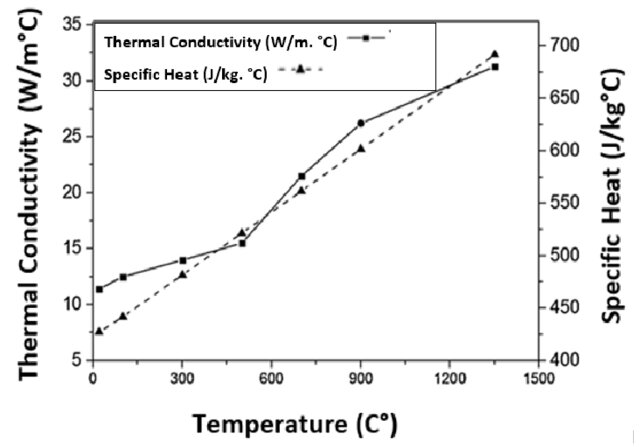
\includegraphics[width=0.75\linewidth]{Images/inconelthermalconductivity.png}
    \caption{Inconel Thermal Conductivity vs Temperature}
    \label{fig:inconel_thermal_conductivity}
\end{figure}

\begin{figure}[H]
    \centering
    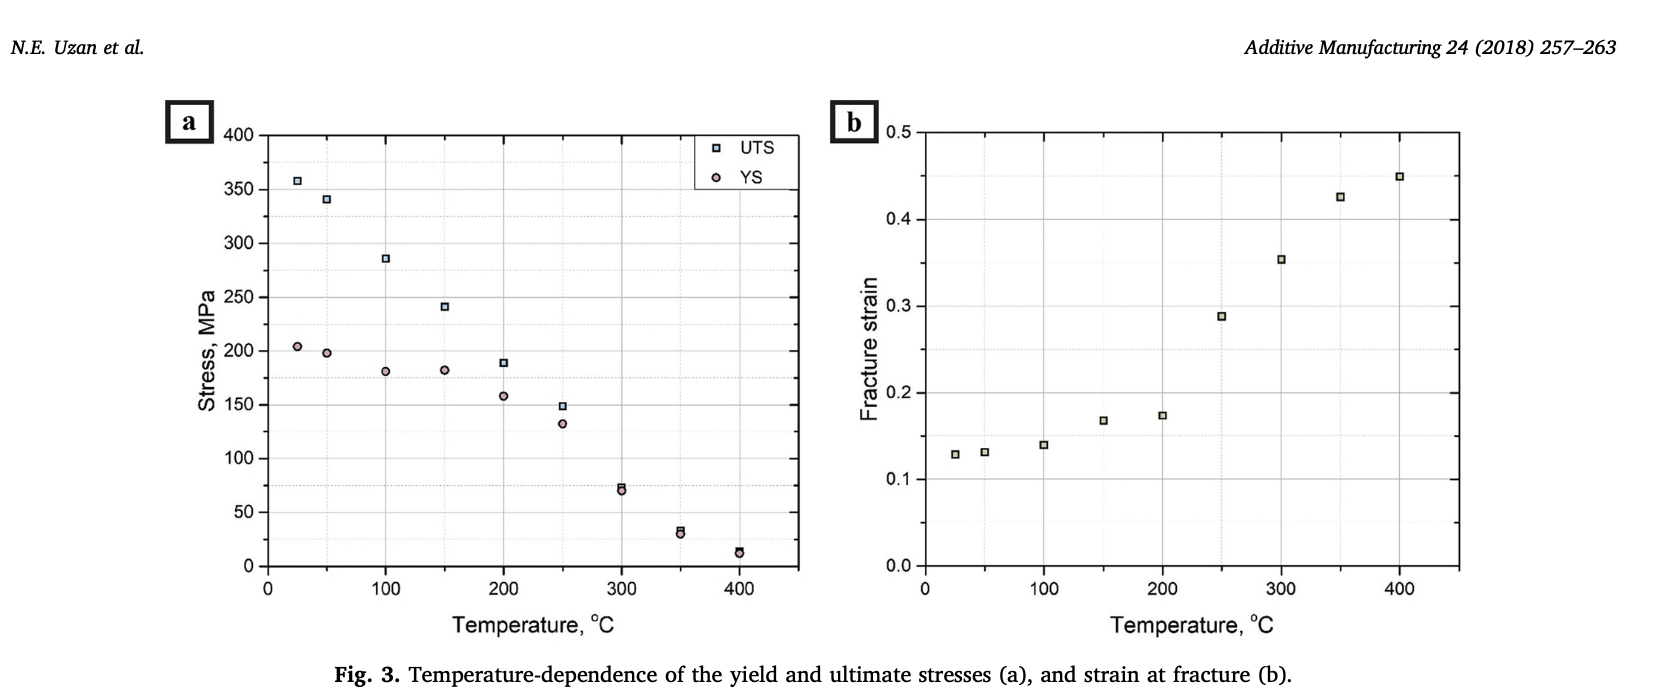
\includegraphics[width=\linewidth]{Images/aluminumstrength.png}
    \caption{AlSi10Mg Strength vs Temperature}
    \label{fig:aluminum_strength}
\end{figure}




\section{Cooling Channel Design}
\subsection{Input Parameters}
\begin{itemize}
    \item \textbf{Chamber Mass Flux:} 
    \[
    \dot{m}_{\text{chamber}} = 3.2574 \, \si{\kilo\gram\per\second} \quad \text{(from RPA)}
    \]
    \item \textbf{Cooling Fraction:} 
    \[
    f_{\text{cool}} = 0.053
    \]
    \item \textbf{Fuel Injector Mass Flow Rate:} 
    \[
    \dot{m}_{\text{fuel, injector}} = 0.6786 \, \si{\kilo\gram\per\second}
    \]
\end{itemize}

The total fuel mass flow rate is:

\[
\dot{m}_{\text{cool}} = f_{\text{cool}} \cdot \dot{m}_{\text{chamber}} = 0.053 \times 3.2574 = 0.1726 \, \si{\kilo\gram\per\second}
\]

\[
\dot{m}_{\text{total}} = \dot{m}_{\text{fuel, injector}} + \dot{m}_{\text{cool}} = 0.6786 + 0.1726 = 0.8512 \, \si{\kilo\gram\per\second}
\]

The percentage of fuel used for regenerative cooling is:

\[
\text{Percent for Regenerative Cooling} = \frac{\dot{m}_{\text{total}}}{\dot{m}_{\text{chamber}}} = \frac{0.8512}{3.2574} = 0.2612 \, \text{or} \, 26.1\%
\]


\section{Cooling Channel Geometry}
\begin{figure}[H]
    \centering
    \includegraphics[width=0.8\textwidth]{Images/CrossSectChannel.png}
    \caption{Cross-sectional view of the cooling channels. Highlights the thermal management design for heat dissipation during combustion.}
    \label{fig:cooling_channels}
\end{figure}

\begin{figure}
    \centering
    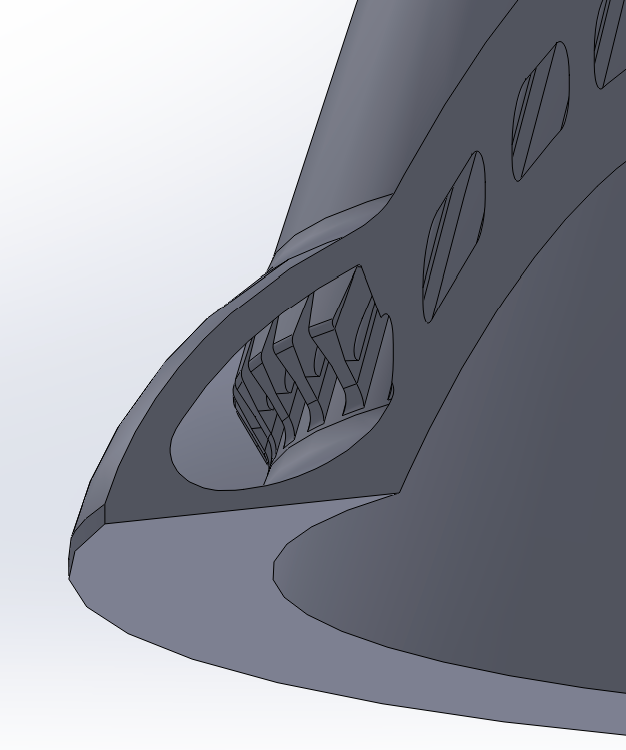
\includegraphics[width=0.75\linewidth]{Images/coolmanifold.png}
    \caption{Nozzle Coolant Distribution Manifold}
    \label{fig:enter-label}
\end{figure}
Optimal Cooling Channel Geometry was determined by RPA based on a 1.5mm wall thickness. 


\begin{itemize}
    \item \textbf{Channel Length:} 
    \[
    L = 0.25 \, \si{\meter}
    \]
    \item \textbf{Number of Channels:} 
    \[
    N = 58
    \]
    \item \textbf{Cross-sectional Area (from CAD):} 
    \[
    A_{\text{channel}} = 2.66291 \times 10^{-6} \, \si{\meter^2}
    \]
    \item \textbf{Perimeter (from CAD):} 
    \[
    P = 5.938 \times 10^{-3} \, \si{\meter}
    \]
\end{itemize}

\textit{Note:} The perimeter was calculated by taking the cross-section of the cooling channels at the smallest area, located around the throat. This design was intentional because thinner channels at the throat increase flow velocity, which enhances heat transfer from the walls to the fluid.

The hydraulic diameter is:

\[
D_h = \frac{4A_{\text{channel}}}{P} = \frac{4 \times 2.66291 \times 10^{-6}}{5.938 \times 10^{-3}} = 1.794 \times 10^{-3} \, \si{\meter}
\]


\subsection{Regen Channel Flow Calculations}

The volumetric flow rate per channel is:

\[
Q = \frac{\dot{m}_{\text{total}}}{\rho N} = \frac{0.8512}{780 \times 58} = 1.904 \times 10^{-5} \, \si{\meter^3\per\second}
\]

The flow velocity is:

\[
v = \frac{Q}{A_{\text{channel}}} = \frac{1.904 \times 10^{-5}}{2.66291 \times 10^{-6}} = 7.07 \, \si{\meter\per\second}
\]

The Reynolds number is:

\[
Re = \frac{\rho v D_h}{\mu} = \frac{780 \times 7.07 \times 1.794 \times 10^{-3}}{0.001095} = 9028.82
\]



\subsubsection{Friction Factor Calculation}

The friction factor depends on the flow regime:

\begin{itemize}
    \item \textbf{Laminar Flow} ($Re < 2300$): 
    \[
    f = \frac{64}{Re}
    \]
    
    \item \textbf{Transitional Flow} ($2300 \leq Re < 4000$): \\
    Using the Blasius approximation:
    \[
    f = 0.079 \cdot Re^{-0.25}
    \]
    
    \item \textbf{Turbulent Flow} ($Re \geq 4000$): \\
    Using the Colebrook-White equation:
    \[
    \frac{1}{\sqrt{f}} = -2 \log_{10} \left(\frac{\epsilon}{3.7D_h} + \frac{2.51}{Re \sqrt{f}} \right)
    \]
\end{itemize}

Given the calculated Reynolds number \(Re = 9028.82\), the flow is turbulent. Solving the Colebrook-White equation numerically yields:

\[
f = 0.0629
\]



\subsubsection{Pressure Drop using Darcy-Weisbach Equation}

The Darcy-Weisbach equation is:

\[
\Delta P = f \cdot \frac{L}{D_h} \cdot \frac{\rho v^2}{2}
\]

Substituting the known values:

\[
\Delta P = 0.0629 \cdot \frac{0.25}{1.794 \times 10^{-3}} \cdot \frac{780 \cdot 7.07^2}{2}
\]

Simplifying:

\[
\Delta P = 1.707 \times 10^5 \, \si{\pascal}
\]

Converting to PSI:

\[
\Delta P_{\text{PSI}} = \frac{\Delta P}{6894.76} = 24.76 \, \si{psi}
\]


\subsubsection{Regen Channel Flow Results Summary}

\begin{itemize}
    \item \textbf{Total Fuel Mass Flow Rate:} \(\dot{m}_{\text{total}} = 0.85 \, \si{\kilo\gram\per\second}\)
    \item \textbf{Reynolds Number:} \(Re = 9028.82 \, \text{(Turbulent)}\)
    \item \textbf{Flow Velocity:} \(v = 7.07 \, \si{\meter\per\second}\)
    \item \textbf{Friction Factor:} \(f = 0.0629\)
    \item \textbf{Pressure Loss:} \(\Delta P = 1.707 \times 10^5 \, \si{\pascal}\)
    \item \textbf{Pressure Loss in PSI:} \(\Delta P_{\text{PSI}} = 24.76 \, \si{psi}\)
\end{itemize}
\subsection{Structural Analysis of Cooling Channels}


\begin{table}[H]
\centering
\begin{tabular}{|l|c|c|}
\hline
\textbf{Parameter} & \textbf{Symbol} & \textbf{Value} \\ 
\hline
Chamber Pressure & $P_c$ & $350 \, \si{psi} = 2.413 \times 10^6 \, \si{Pa}$ \\ 
\hline
Fuel Maximum Expected Operating Pressure (MEOP) & $P_f$ & $1000 \, \si{psi} = 6.895 \times 10^6 \, \si{Pa}$ \\ 
\hline
Minimum Wall Thickness & $t$ & $0.0015 \, \si{m}$ \\ 
\hline
Cooling Channel Inner Radius & $r_i$ & $0.046 \, \si{m}$ \\ 
\hline
Cooling Channel Width & $r_{\text{cooling}}$ & $0.0015 \, \si{m}$ \\ 
\hline
Material Allowable Yield Strength at 250$^\circ$C (AlSi10Mg) & $\sigma_{\text{allow}}$ & $125 \times 10^6 \, \si{Pa}$ \\ 
\hline
Safety Factor & $SF$ & 1.5 \\ 
\hline
\end{tabular}
\caption{Design Parameters for Structural and Thermal Calculations}
\label{tab:given_parameters}
\end{table}


\subsubsection{Cooling Channel Hoop Stress}

The hoop stress in the cooling channel wall is calculated using the thin-walled pressure vessel approximation:

\[
\sigma_{\text{cool}} = \frac{P_c \cdot SF \cdot r_{\text{cooling}}}{t}
\]

Substituting values:

\[
\sigma_{\text{cool}} = \frac{2.413 \times 10^6 \times 1.5 \times 0.0015}{0.0015} = 3.62 \times 10^6 \, \si{Pa} = 3.62 \, \si{MPa}
\]

\subsubsection{Outer Wall Stress}

The outer wall stress is calculated as:

\[
\sigma_{\text{main}} = \frac{P_f \cdot SF \cdot r_i}{t}
\]

Substituting values:

\[
\sigma_{\text{main}} = \frac{6.895 \times 10^6 \times 1.5 \times 0.046}{0.0015} = 1.1101 \times 10^8 \, \si{Pa} = 111.01 \, \si{MPa}
\]

Margin of Safety

The margin of safety is given by:

\[
\text{Margin} = \frac{\sigma_{\text{allow}}}{\sigma_{\text{main}}} - 1
\]

Substituting values:

\[
\text{Margin} = \frac{125 \times 10^6}{1.1101 \times 10^8} - 1 = 0.126 = 12.60\%
\]

\subsubsection{Cooling Channel Structural Results}

\begin{itemize}
    \item \textbf{Cooling Channel Stress:} \(\sigma_{\text{cool}} = 3.62 \, \si{MPa}\)
    \item \textbf{Outer Wall Stress:} \(\sigma_{\text{main}} = 111.01 \, \si{MPa}\)
    \item \textbf{Material Allowable Stress:} \(\sigma_{\text{allow}} = 125 \, \si{MPa}\)
    \item \textbf{Margin of Safety:} \(\text{Margin} = 12.60\%\)
\end{itemize}
\begin{figure}
    \centering
    \includegraphics[width=0.75\linewidth]{Images/{B956974B-11EA-41F3-90EC-EB3121FBE316}.png}
    \caption{FEA Analysis}
    \label{fig:enter-label}
\end{figure}
FEA results show a higher peak stress, but this is at a nonphysical mesh location. 


\section{Ethanol Pintle Flow Calculations}

\begin{table}[H]
\centering
\begin{tabular}{|l|c|c|}
\hline
\textbf{Parameter} & \textbf{Symbol} & \textbf{Value} \\ 
\hline
Discharge Coefficient (From ICL Technical Report) & $C_d$ & $0.82$ \\ 
\hline
Ethanol Density & $\rho$ & $780 \, \si{\kilo\gram\per\meter^3}$ \\ 
\hline
Orifice Inner Diameter (Given) & $d_{\text{inner}}$ & $0.74525 \, \si{inches} = 0.01893 \, \si{m}$ \\ 
\hline
Desired Mass Flow Rate & $\dot{m}_{\text{desired}}$ & $0.68 \, \si{\kilo\gram\per\second}$ \\ 
\hline
Upstream Pressure & $P_1$ & $700 \, \si{psi} = 4.826 \times 10^6 \, \si{Pa}$ \\ 
\hline
Downstream Pressure & $P_2$ & $350 \, \si{psi} = 2.413 \times 10^6 \, \si{Pa}$ \\ 
\hline
Pressure Drop & $\Delta P$ & $350 \, \si{psi} = 2.413 \times 10^6 \, \si{Pa}$ \\ 
\hline
\end{tabular}
\caption{Pintle Fuel Flow Rate Design Parameters}
\label{tab:orifice_parameters}
\end{table}

\subsection{Pintle Gap Calculation}

The outer diameter of the annular orifice is determined by:

\[
d_{\text{outer}} = d_{\text{inner}} + 2 \cdot g
\]

Where:
\begin{itemize}
    \item \( d_{\text{outer}} \): Outer diameter of the annular gap (m)
    \item \( d_{\text{inner}} \): Inner diameter of the orifice (m)
    \item \( g \): Pintle gap (m)
\end{itemize}

The annular flow area is calculated as:

\[
A = \frac{\pi}{4} \left(d_{\text{outer}}^2 - d_{\text{inner}}^2 \right)
\]

The volumetric flow rate is:

\[
Q = C_d \cdot A \cdot \sqrt{\frac{2 \Delta P}{\rho}}
\]

The corresponding mass flow rate is:

\[
\dot{m} = \rho Q = \rho \cdot C_d \cdot A \cdot \sqrt{\frac{2 \Delta P}{\rho}}
\]

Solving this equation for the pintle gap \( g \), the MATLAB numerical solution yields:

\[
g = 0.000223 \, \si{\meter} = 0.008793 \, \si{inches}
\]



\subsection{Pintle Gap Results}

\begin{itemize}
    \item \textbf{Desired Mass Flow Rate:} \(\dot{m}_{\text{desired}} = 0.68 \, \si{\kilo\gram\per\second}\)
    \item \textbf{Pressure Drop:} \(\Delta P = 350 \, \si{psi}\)
    \item \textbf{Orifice Inner Diameter:} \(d_{\text{inner}} = 0.74525 \, \si{inches}\)
    \item \textbf{Calculated Pintle Gap:} 
    \[
    g = 0.000223 \, \si{\meter} = 0.008793 \, \si{inches}
    \]
\end{itemize}



\section{Throttle Level Thermal Profiles}

Throttling significantly decreases the regen flow rates, but does not decrease combustion temperature. This poses a significant challenge as the engine would otherwise melt at low throttle levels. If fuel and oxidizer can be throttled independently, the OF ratio can be programmed to shift more fuel rich when a low throttle maneuver is commanded. This will decrease combustion temperature as well as maintain nominal regenerative cooling flow. The film cooling can also be independent of throttle level if the engine is throttled by moving the pintle components directly rather than throttling upstream of the engine by closing valves. For precision landing scenarios like the Lunar Lander Challenge, where the engine may need to operate at as low as 12\% to achieve a thrust-to-weight (T/W) ratio of 1 for a 150-lb vehicle, running fuel-rich under these conditions ensures sustained cooling and prevents thermal failure.

\subsection{Thermal Profiles by Throttle Level}

The following figures present the thermal profiles of the engine at various throttle levels, highlighting the impact of reduced propellant flow on chamber wall temperatures. Each simulation assumes a 1.5 mm chamber wall thickness and an aluminum construction, and a 600 mm characteristic length (L$^*$) with 58 regenerative cooling channels.

\subsubsection{Low Throttle Operation}
\begin{figure}[H]
    \centering
    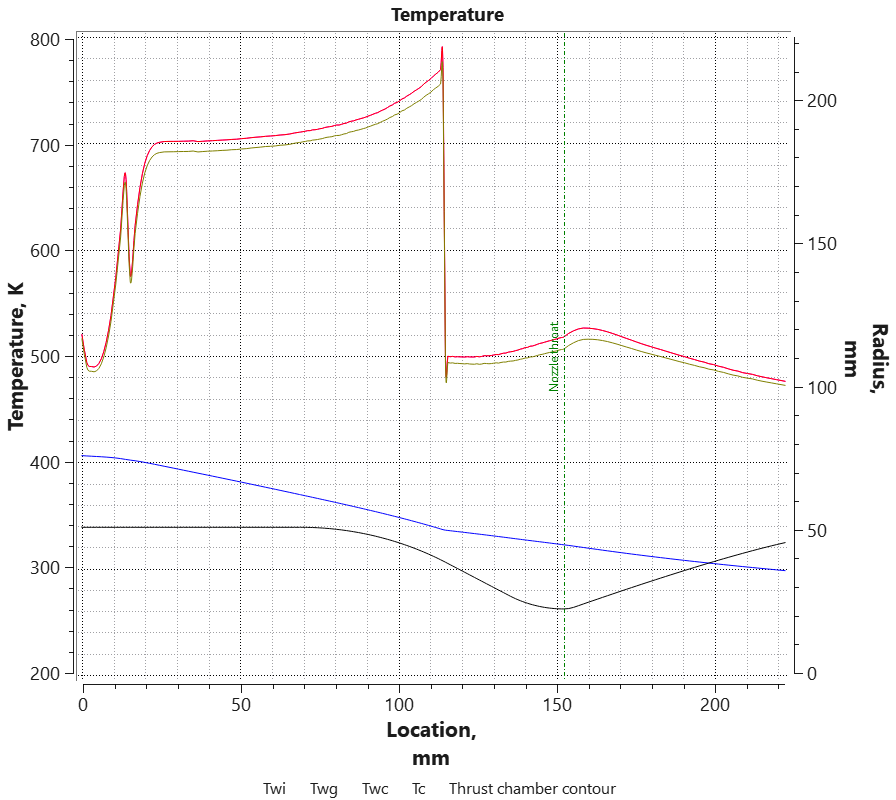
\includegraphics[width=\linewidth]{Images/12_throttle_80_20_2film3.8of_20xfilm_aluminum_1.5mmwall_600Lstar_rao_55channels.png}
    \caption{Thermal Profile at 12\% Throttle}
    \label{fig:12_throttle}
\end{figure}

\begin{figure}[H]
    \centering
    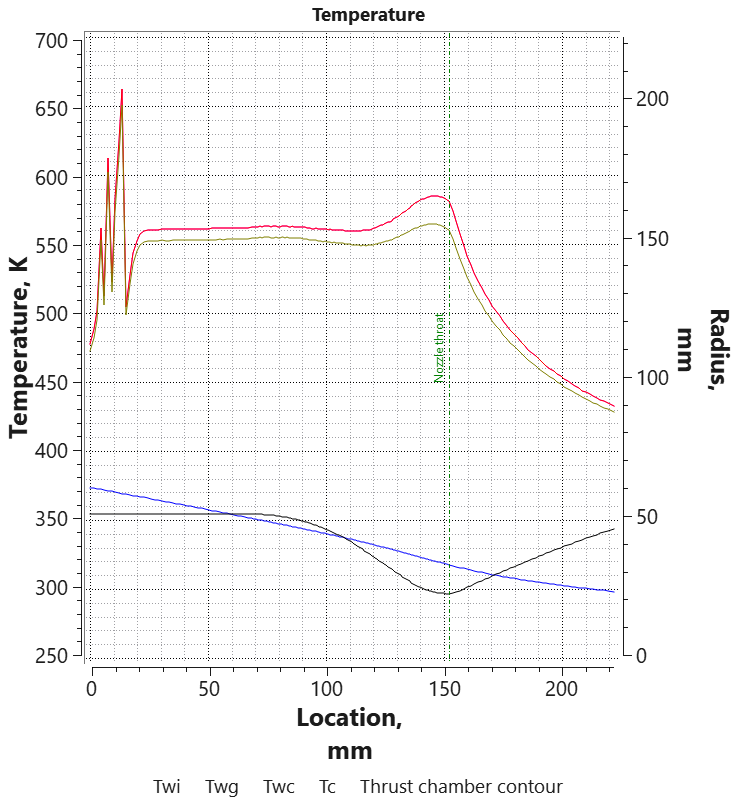
\includegraphics[width=\linewidth]{Images/20_throttle_80_20_2film3.8of_4.8xfilm_aluminum_1.5mmwall_600Lstar_rao_55channels.png}
    \caption{Thermal Profile at 20\% Throttle}
    \label{fig:20_throttle}
\end{figure}

\subsubsection{Mid-Level Throttle Operation}
\begin{figure}[H]
    \centering
    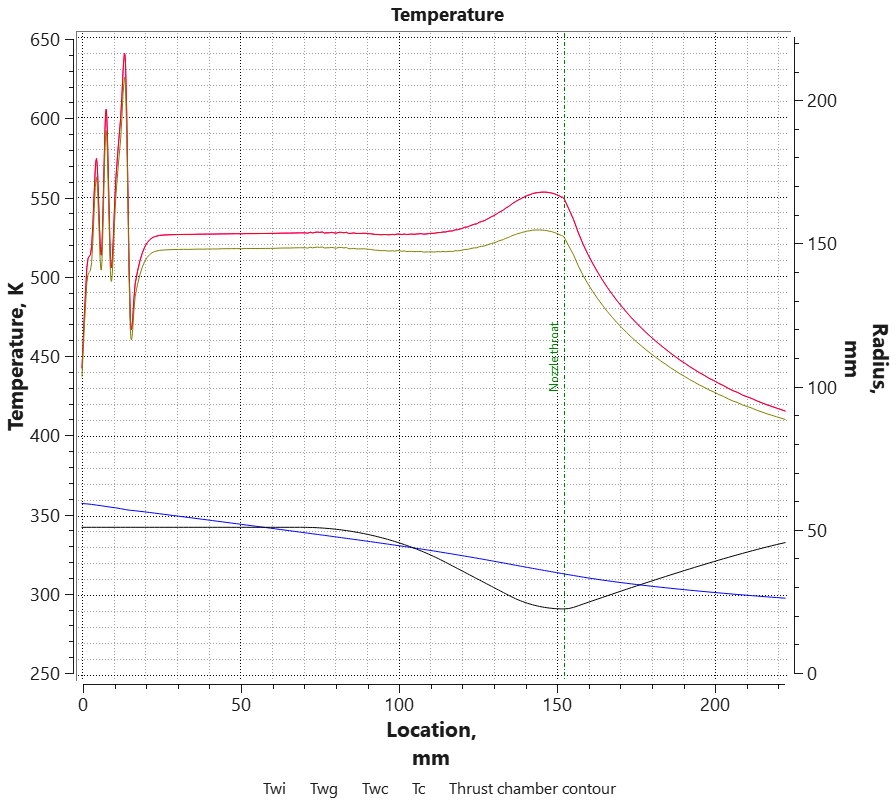
\includegraphics[width=\linewidth]{Images/30_throttle_80_20_2film3.8of_4.8xfilm_aluminum_1.5mmwall_600Lstar_rao_55channels.png}
    \caption{Thermal Profile at 30\% Throttle}
    \label{fig:30_throttle}
\end{figure}

\begin{figure}[H]
    \centering
    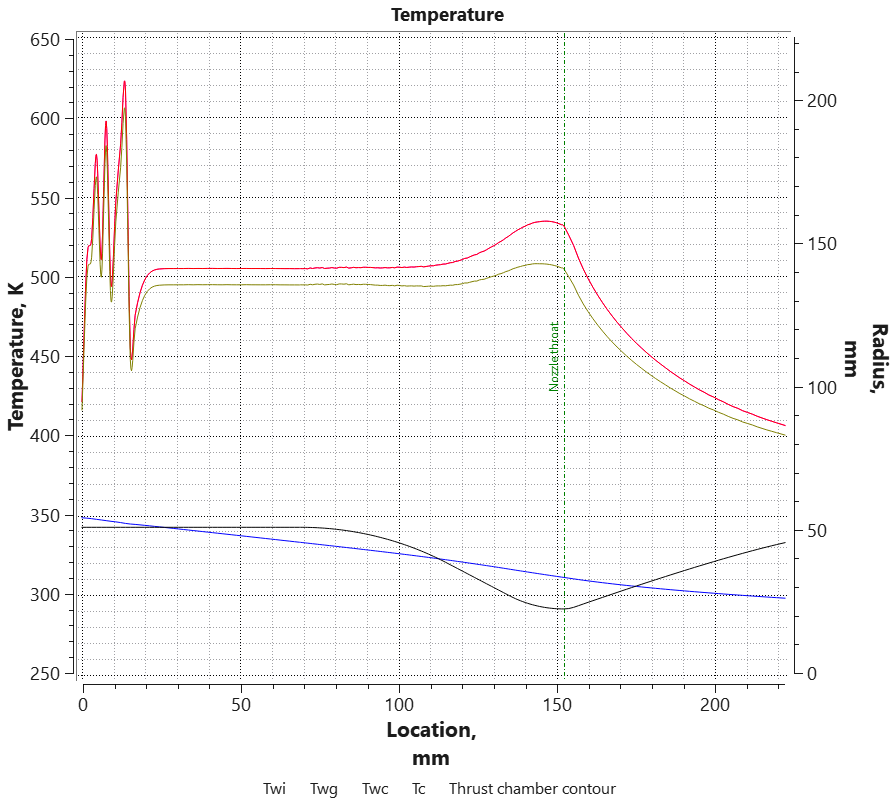
\includegraphics[width=\linewidth]{Images/40_throttle_80_20_2film3.8of_4.8xfilm_aluminum_1.5mmwall_600Lstar_rao_55channels.png}
    \caption{Thermal Profile at 40\% Throttle}
    \label{fig:40_throttle}
\end{figure}

\subsubsection{High Throttle Operation}
\begin{figure}[H]
    \centering
    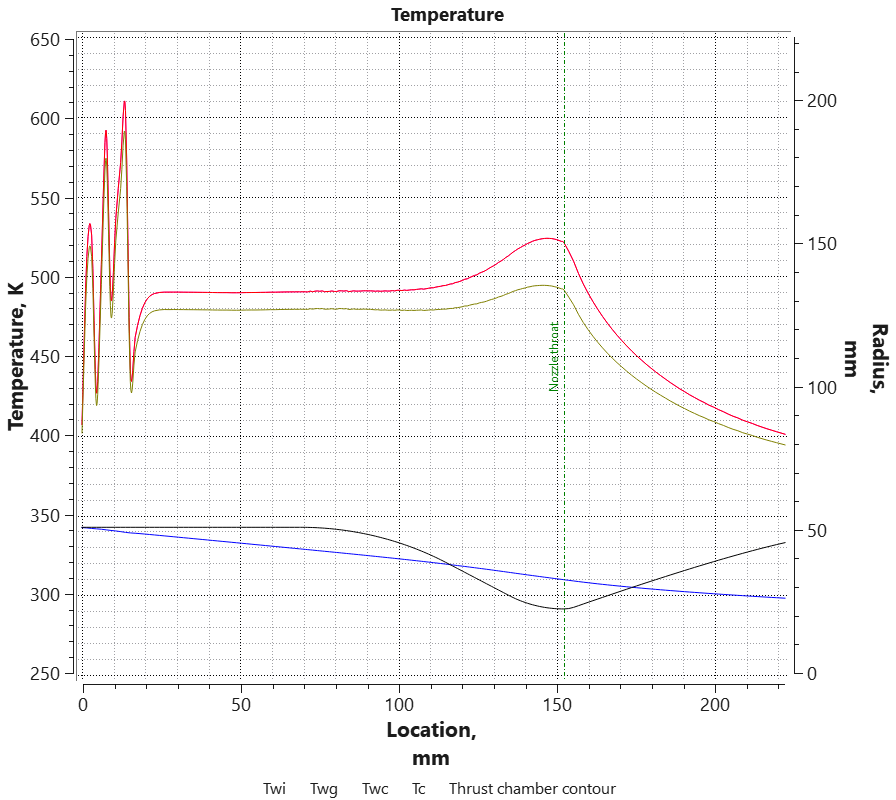
\includegraphics[width=\linewidth]{Images/50_throttle_80_20_2film3.8of_4.8xfilm_aluminum_1.5mmwall_600Lstar_rao_55channels.png}
    \caption{Thermal Profile at 50\% Throttle}
    \label{fig:50_throttle}
\end{figure}
    
\section{MENG Updates}
\section{Design Modifications and CAD Development}

\subsection{Fuel Inlet Modifications}

The fuel inlet port was modified from the original design which was an -08 O-Boss to a -06 O-boss configuration to fit within the $6''$ inscribed circle constraint. This constraint exists so that the rocket engine can fit within CRT's standard airframes. 
\begin{figure}
    \centering
    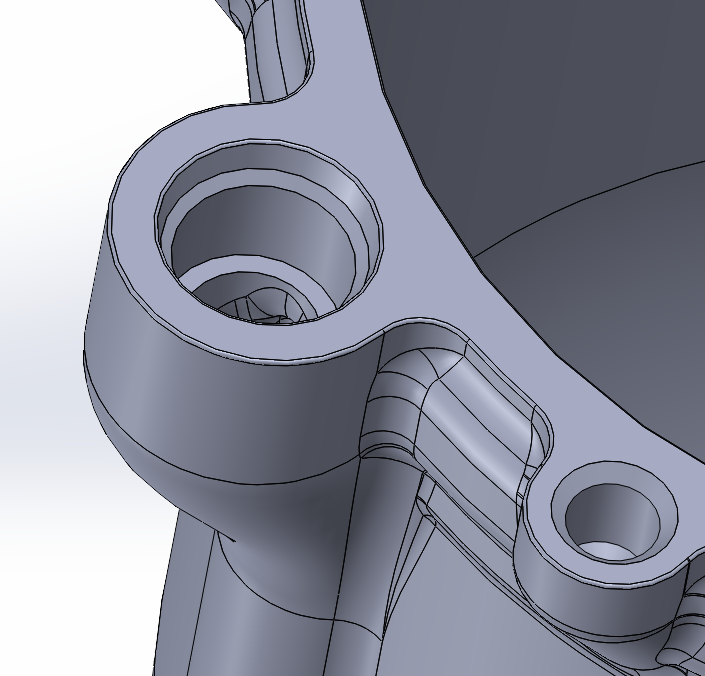
\includegraphics[width=0.5\linewidth]{Images/fuelinlet.png}
    \caption{Fuel Inlet}
    \label{fig:enter-label}
\end{figure}
\subsection{Combustion Chamber Modifications}

Additional improvements to the upper fuel channels included the addition of fillets and a reinforcement band around the injector interface. The original minimum wall thickness was approximately $1\,\text{mm}$, but analysis indicated a requirement of at least $3.3\,\text{mm}$ to achieve a safety factor of 1.5. The final design increased this dimension to $4\,\text{mm}$ ($0.157''$) to provide additional margin.
\begin{figure}
    \centering
    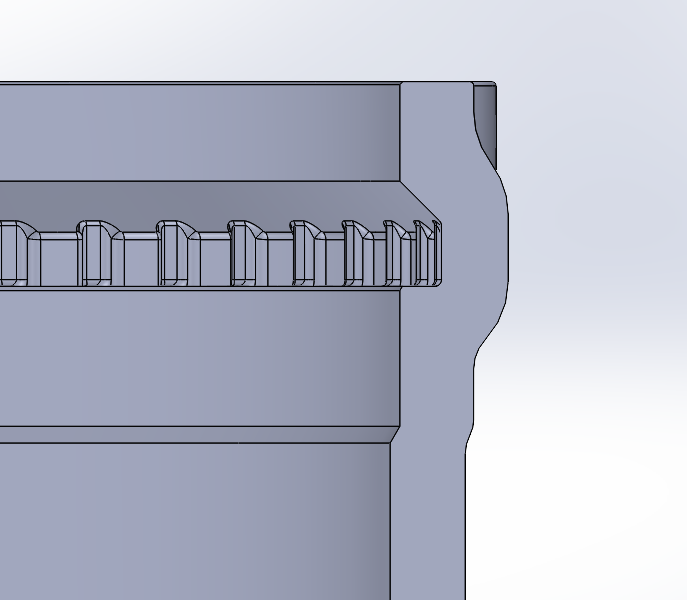
\includegraphics[width=0.5\linewidth]{Images/image.png}
    \caption{Reinforcement Band}
    \label{fig:enter-label}
\end{figure}
\begin{figure}
    \centering
    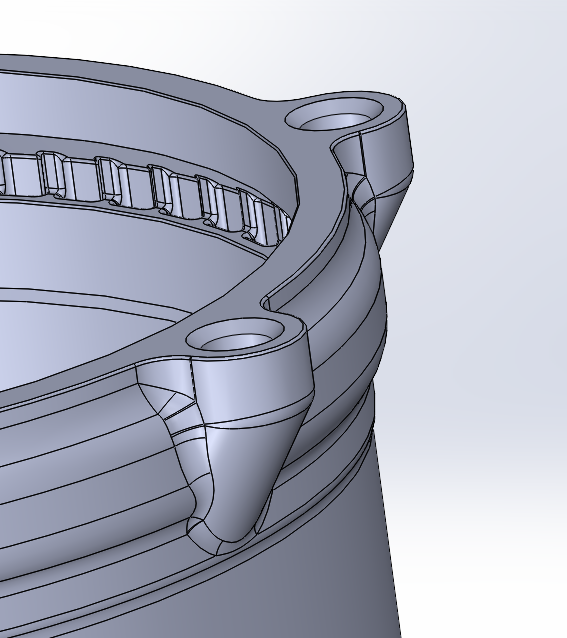
\includegraphics[width=0.5\linewidth]{filletsandreinforementband.png}
    \caption{Fuel Channel Fillets and Reinforcement Band}
    \label{fig:enter-label}
\end{figure}

Manufacturing 

The injector interface dimensions were modified to accommodate an O-ring (size 241). Dimensional tolerance requirements were specified by XMAKE at $\pm0.3\%$ with a minimum of $0.3\,\text{mm}$, meaning potential ID variation of $0.0125$. To account for this variation and to achieve the correct dimensions post machining, the 3D printed model needed to be modified to add additional material around the bore.  The design targets a diametral clearance of 3 thousandths of an inch ($0.003''$) to ensure proper O-ring compression per ORD-5700.  This model also has the bolt holes removed, as they will be post machined as well. 

 

\section{Structural Analysis}

\subsection{FEA Methodology}

A comprehensive Finite Element Analysis (FEA) approach was implemented to verify the structural integrity of the engine design. The primary goal of these analyses was to verify that the combustion chamber will survive the thermal and pressure loads resulting from nominal operation of the engine. The combustion chamber, and the combustion chamber assembly were analyzed using ANSYS Static Structural simulations in three separate models: Isolated Chamber, Combined Chamber and Injector, and sectioned Combined Chamber and Injector. Thermal and structural loads were considered independently, as well as concurrently. The engine was simulated to standard CRT factors of safety. 



\subsection{Isolated Chamber Analysis}
Initial FEA runs on the isolated chamber revealed constraint-related issues causing high stresses in unrealistic locations as seen in As shown in Figure \ref{fig:fixedbolt}. The original ANSYS model for the chamber only consisted of the chamber body, and no other components. However, analyzing the chamber in this way was not accurate. The original model has the bolt holes fixed, but this lead to high stress areas as shown in the figure. To determine whether these stresses were realistic, the bottom was then fixed, and the top was left unconstrained. The stress in the injector interface decreased significantly as seen in Figure \ref{fig:fixedbolt}, however this is an under-conservative estimate, because the constraint on the bolt holes does induce stress in this area of the chamber. This stress is due to the pressure bowing out the areas between the bolts. The degree to which this effect occurs is controlled by the stiffness of the injector.
\begin{figure}
    \centering
    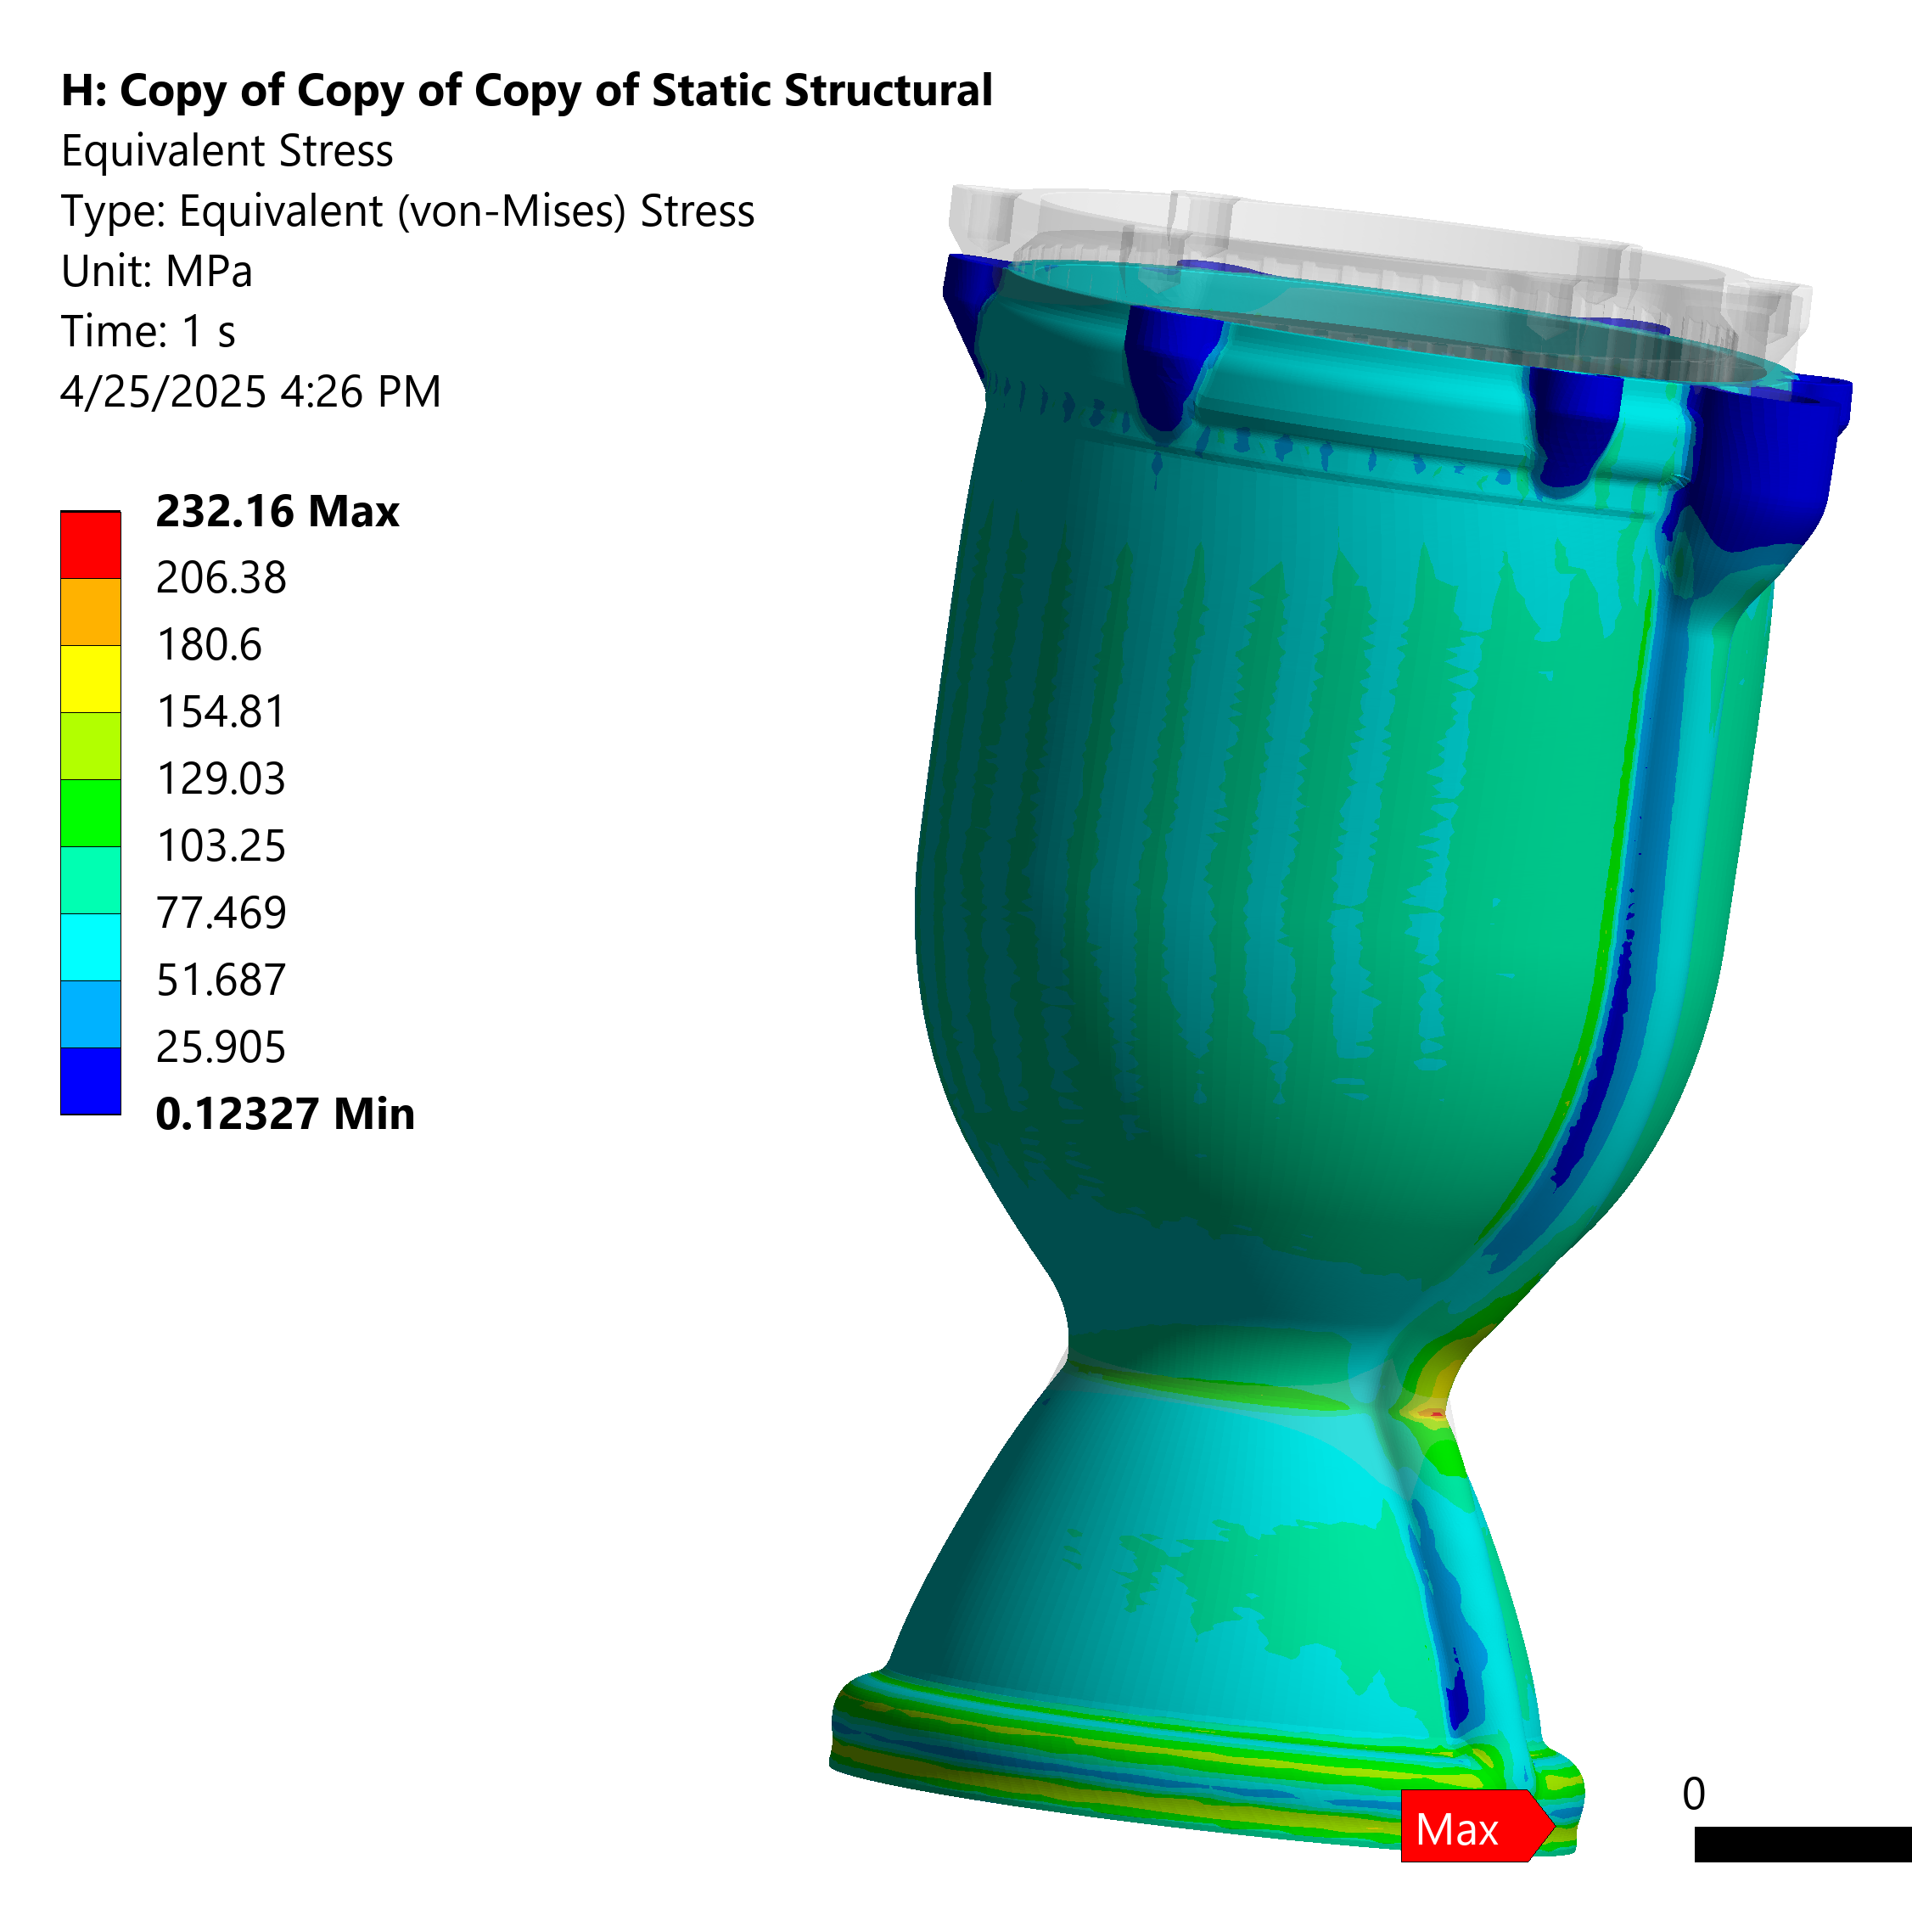
\includegraphics[width=1\linewidth]{bottomfixed.png}
    \caption{Fixed Bottom}
    \label{fig:Fixed Bottom}
\end{figure}
\begin{figure}
    \centering
    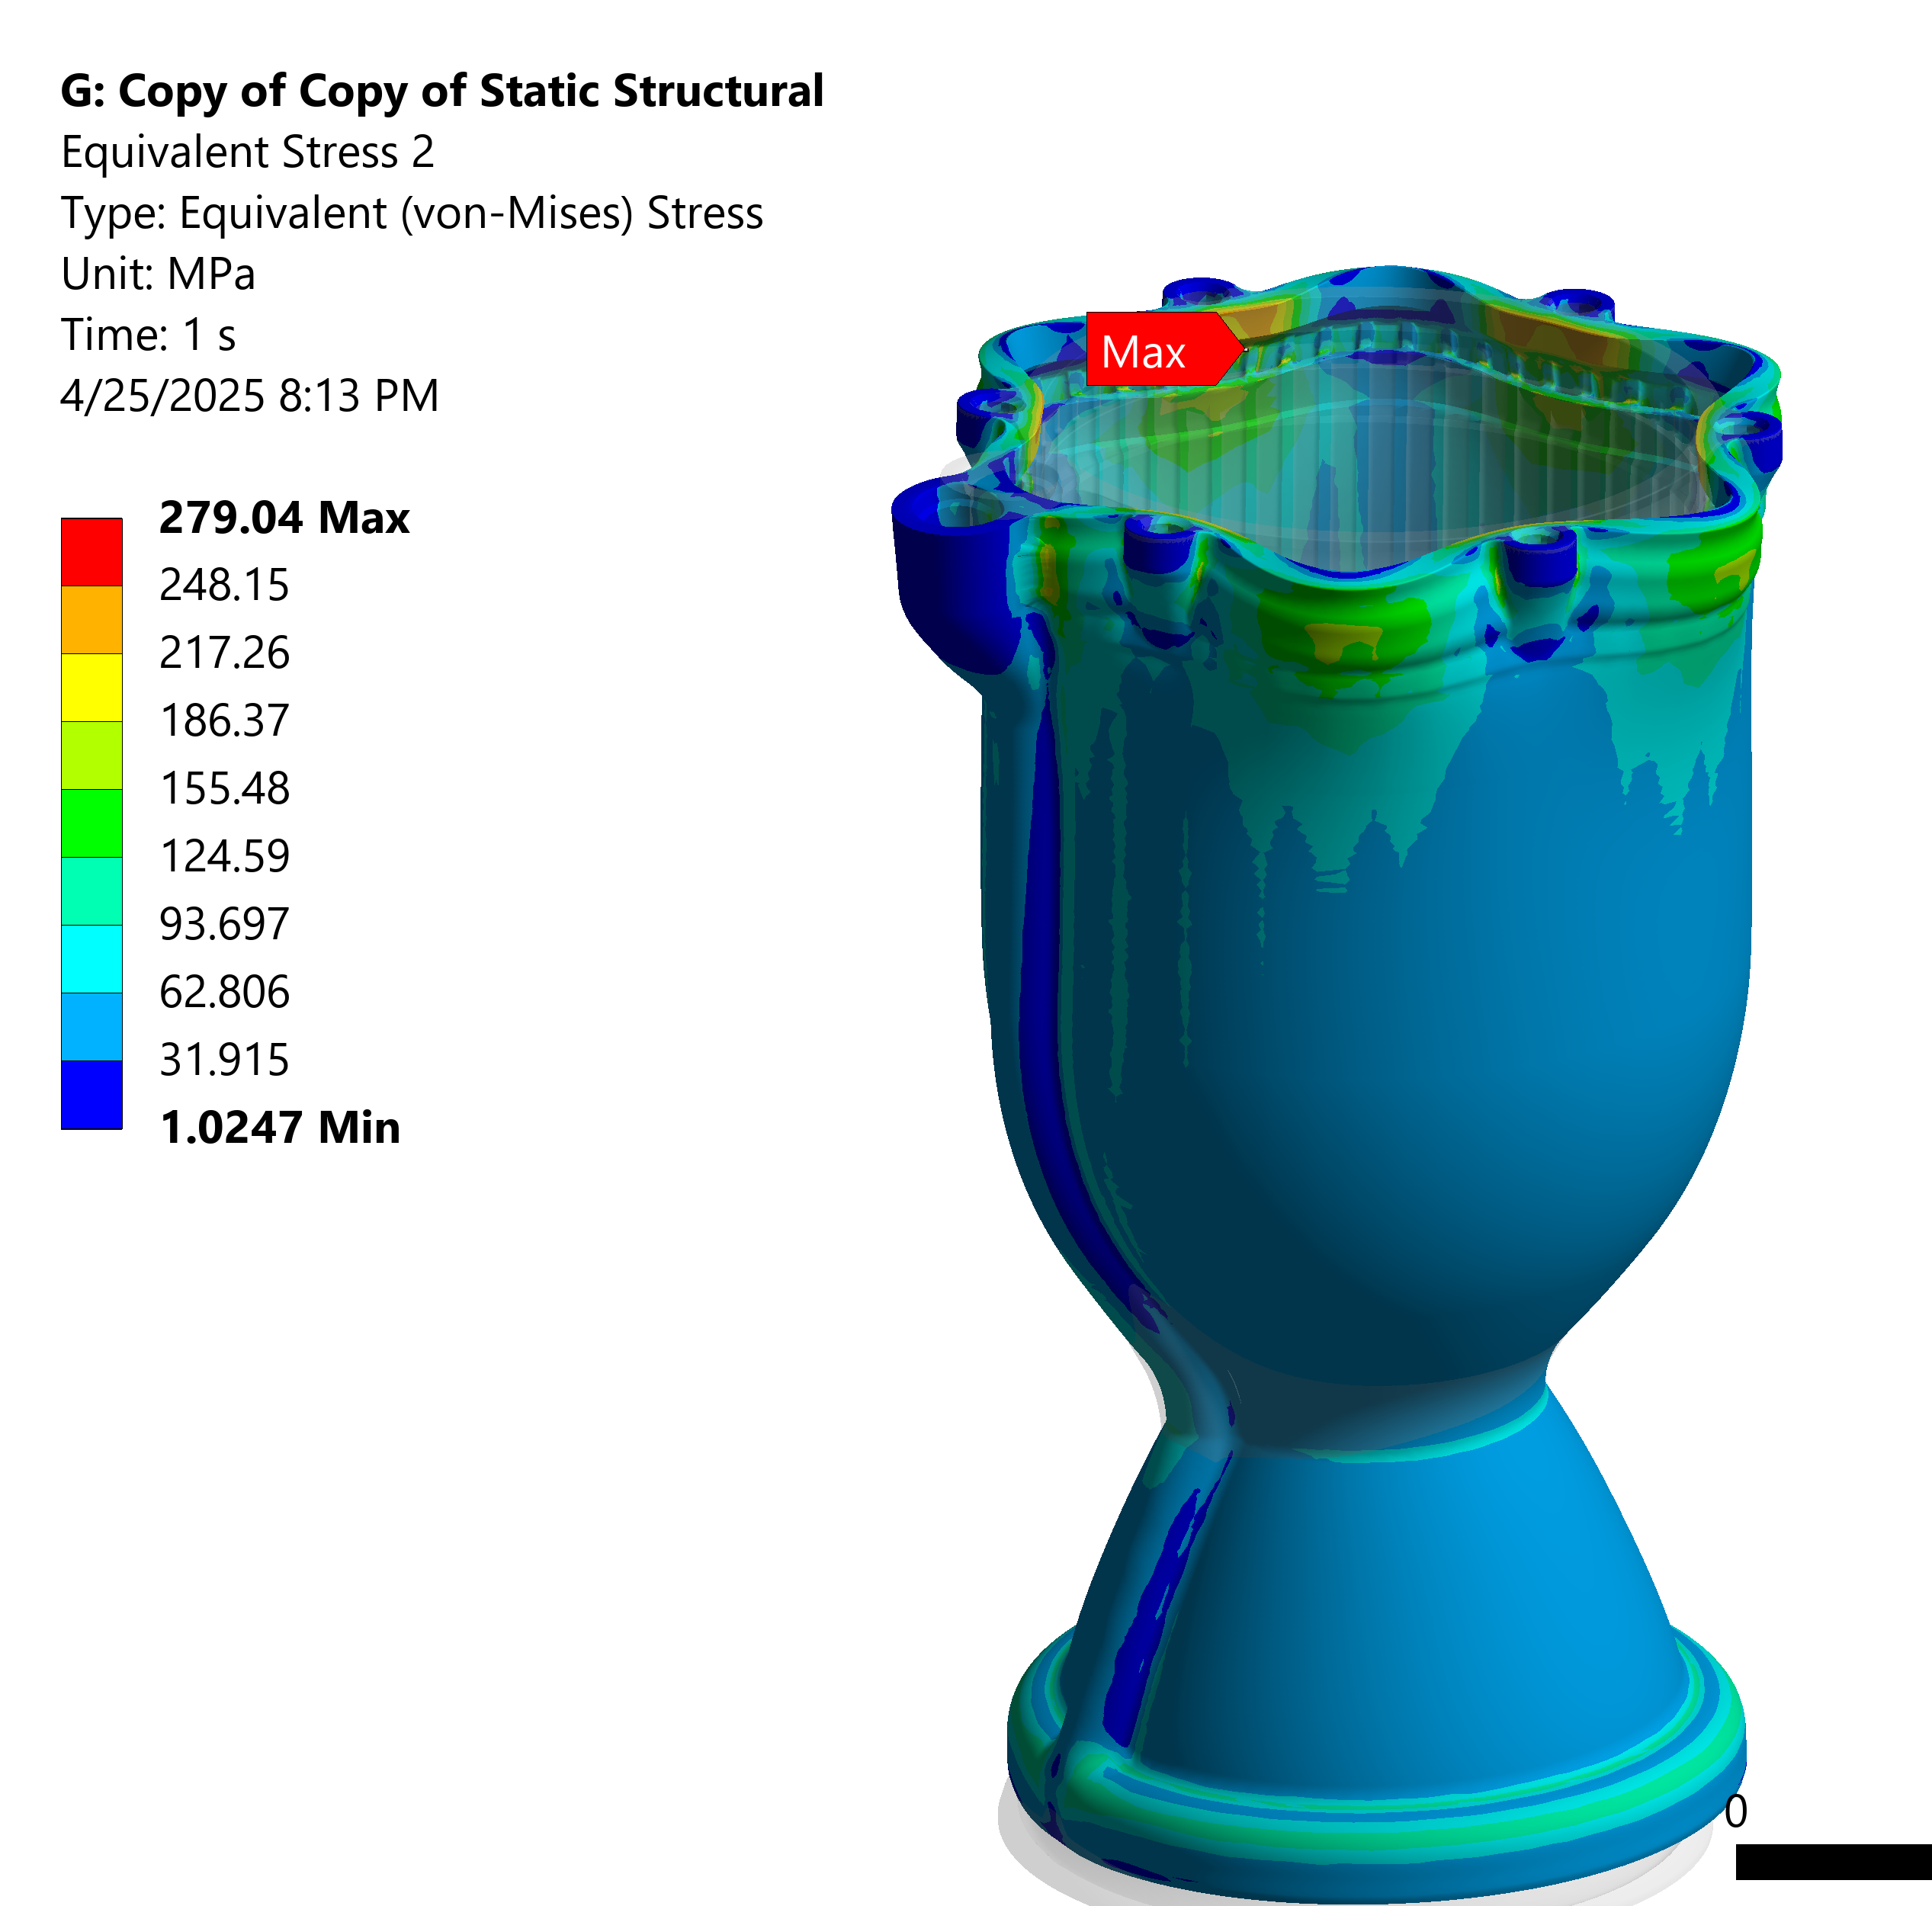
\includegraphics[width=1\linewidth]{isolatedchamber.png}\ref{}
    \caption{Fixed Bolt Constraint}
    \label{fig:fixedbolt}
\end{figure}
 
This prompted refinement of the boundary conditions and constraint methodologies to better represent the actual operating environment. To accurately model this area, the injector was added to the model, along with the bolts.  

\begin{figure}
    \centering
    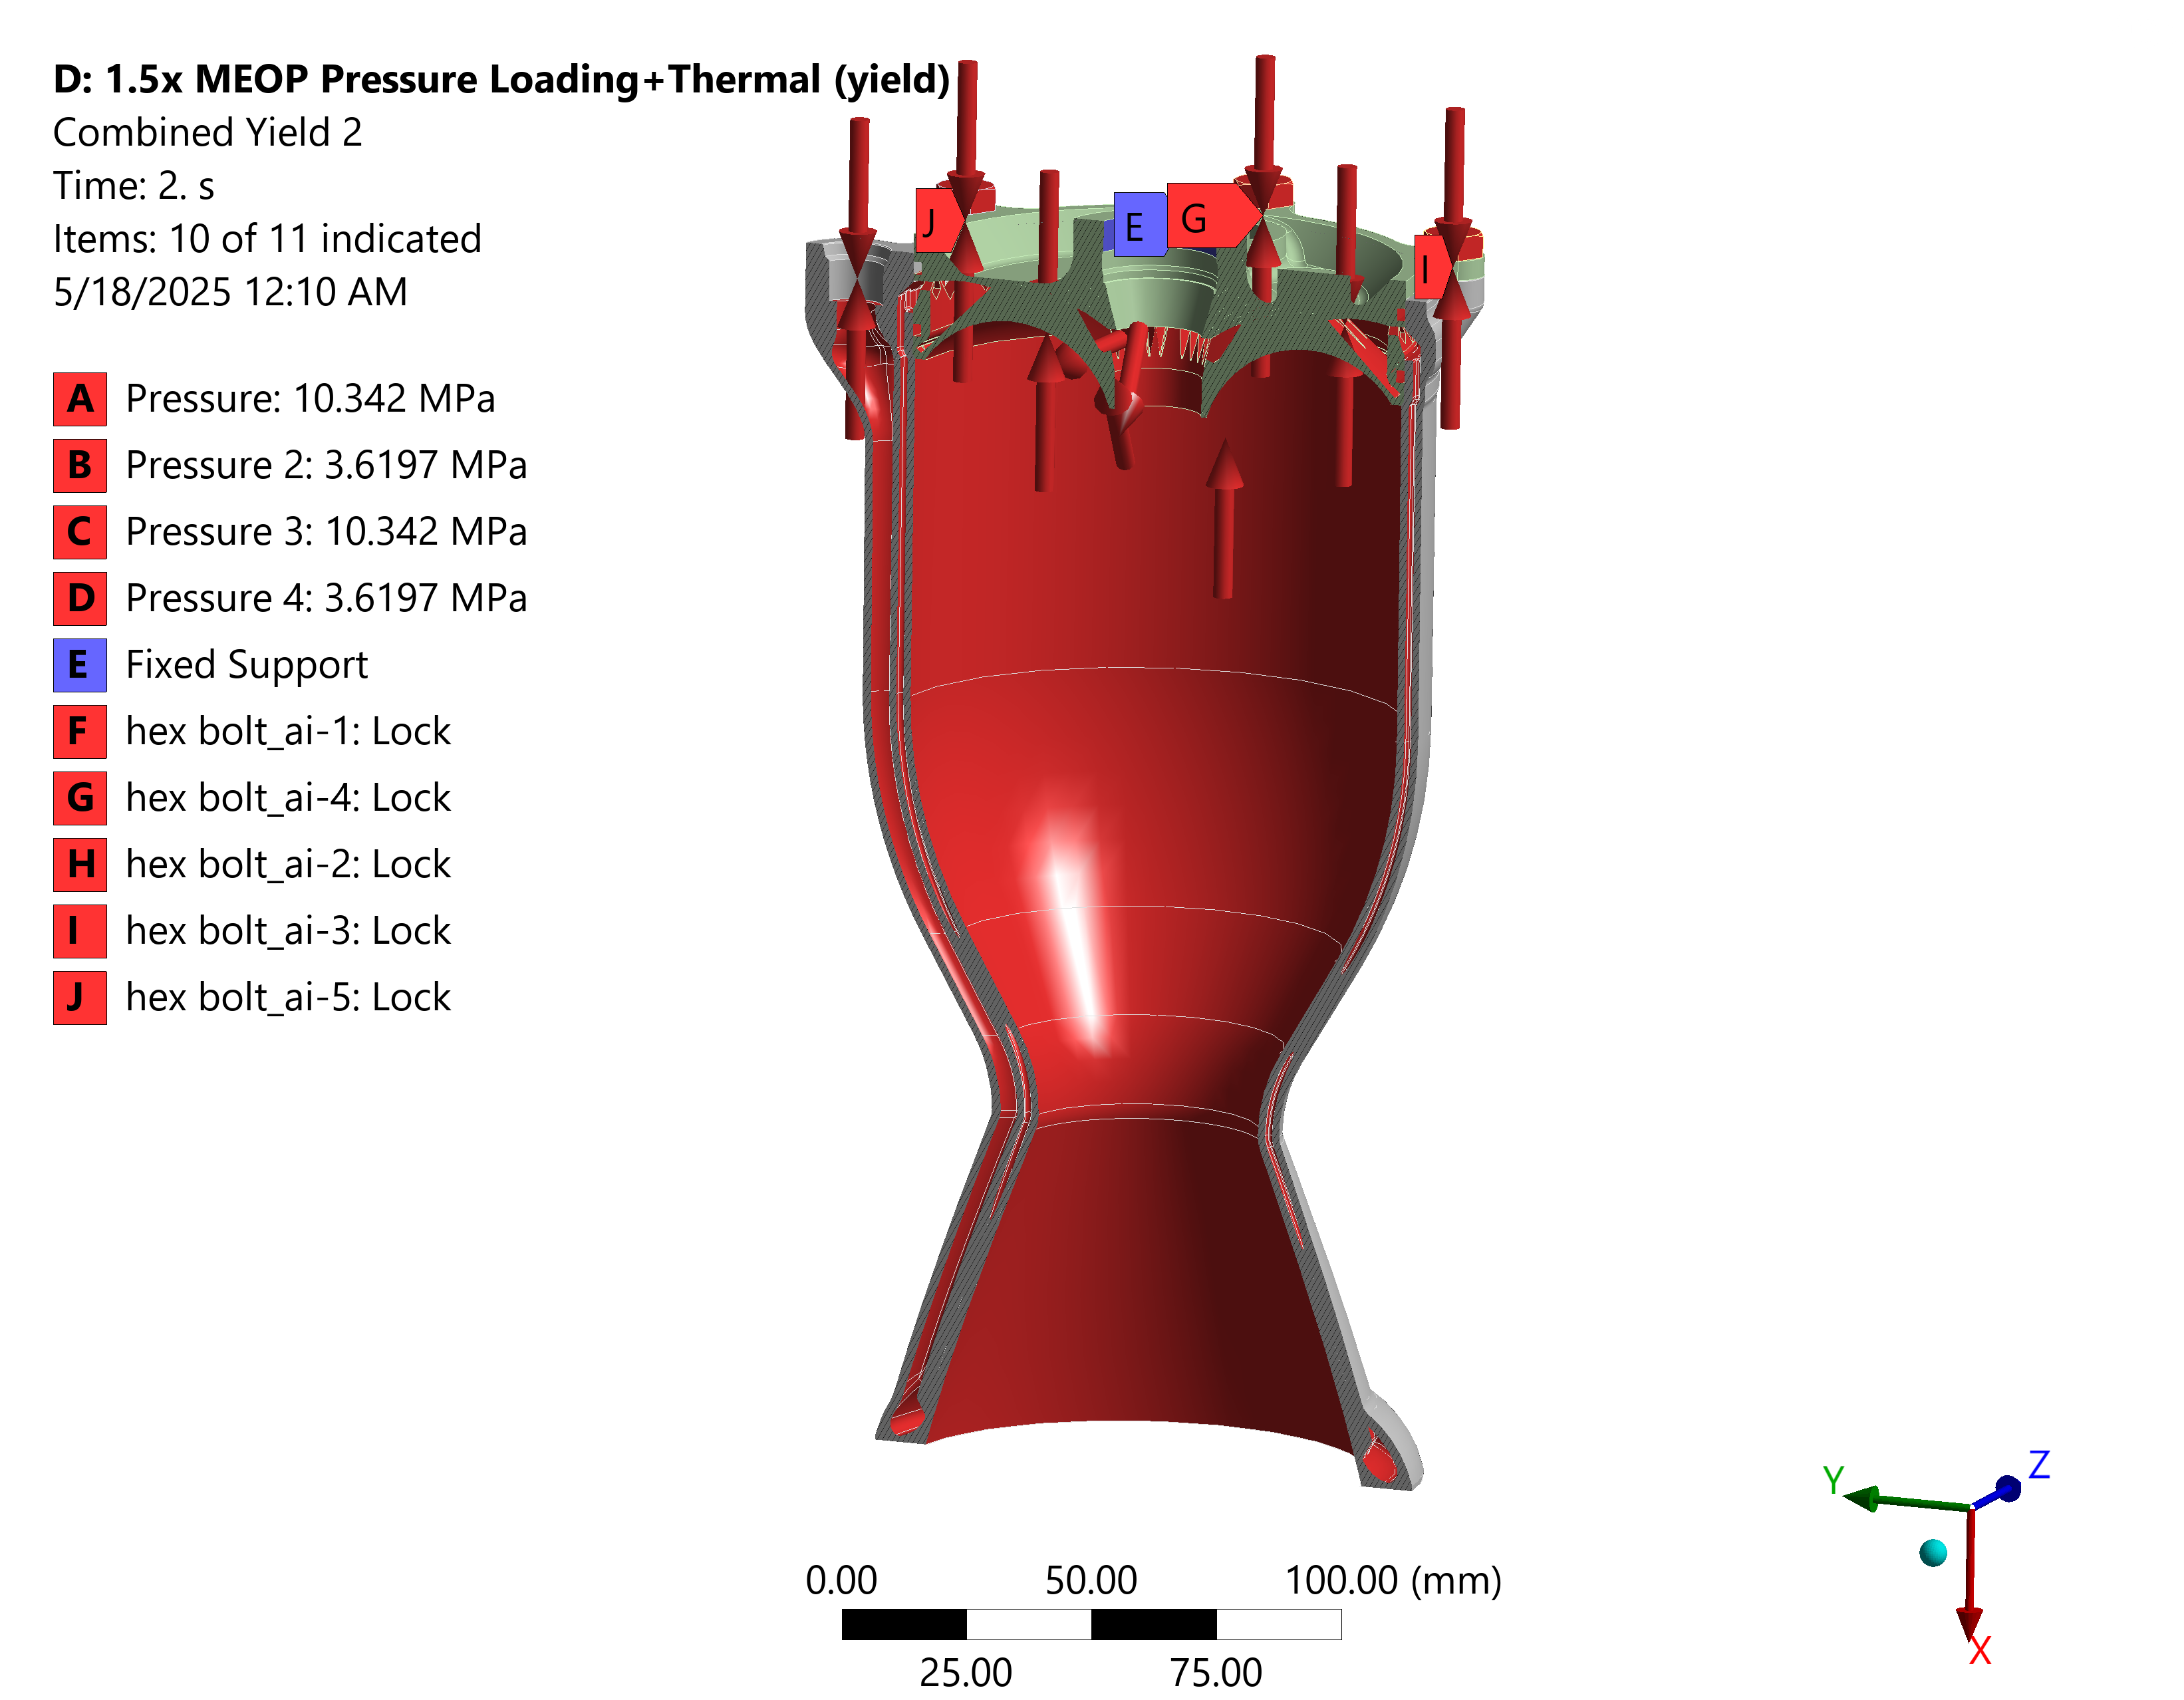
\includegraphics[width=1\linewidth]{Images/CombinedSetup.png}
    \caption{Combined Setup}
    \label{fig:CombinedSetup}
\end{figure}
\subsection{Boundary Conditions}
The following boundary conditions are shared between the breakout sectioned model and the whole combined model, with the exception of the frictionless support added to the breakout sectioned model. 
\begin{figure}
    \centering
    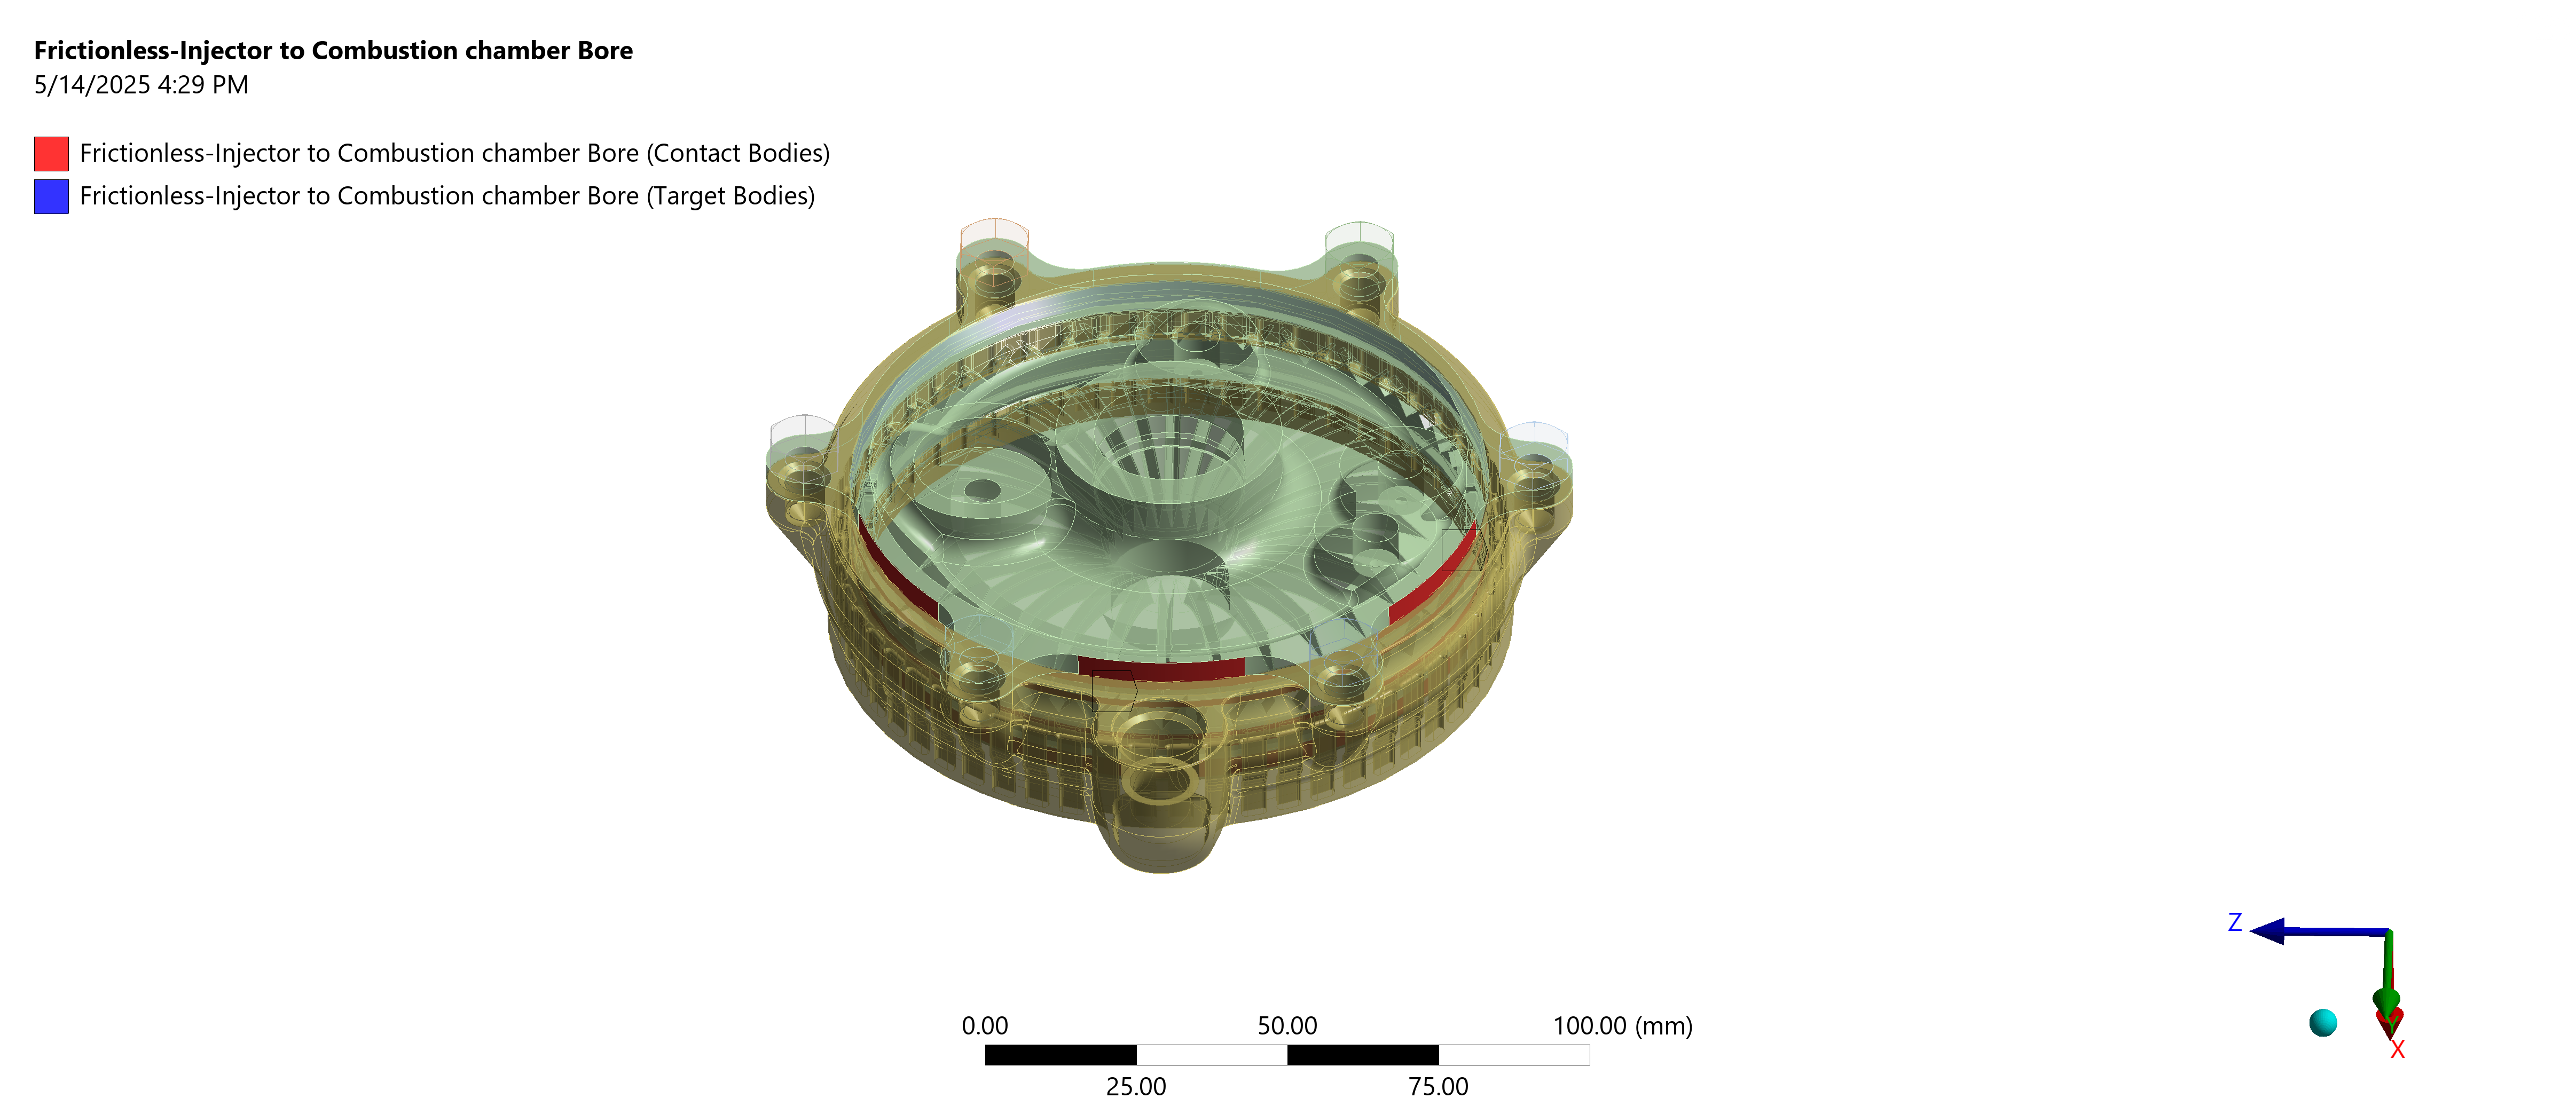
\includegraphics[width=1\linewidth]{Images/Bore Frictionless.png}
    \caption{Frictionless Bore Contact}
    \label{fig:FrictionlessBoreContact}
\end{figure}
This frictionless contact between the bore of the chamber and the injector OD prevents the injector from deflecting through the chamber walls. The bore and injector will be lubricated, and should slide against each-other if they contact. Therefore, frictionless is an appropriate contact scheme. 
\begin{figure}
    \centering
    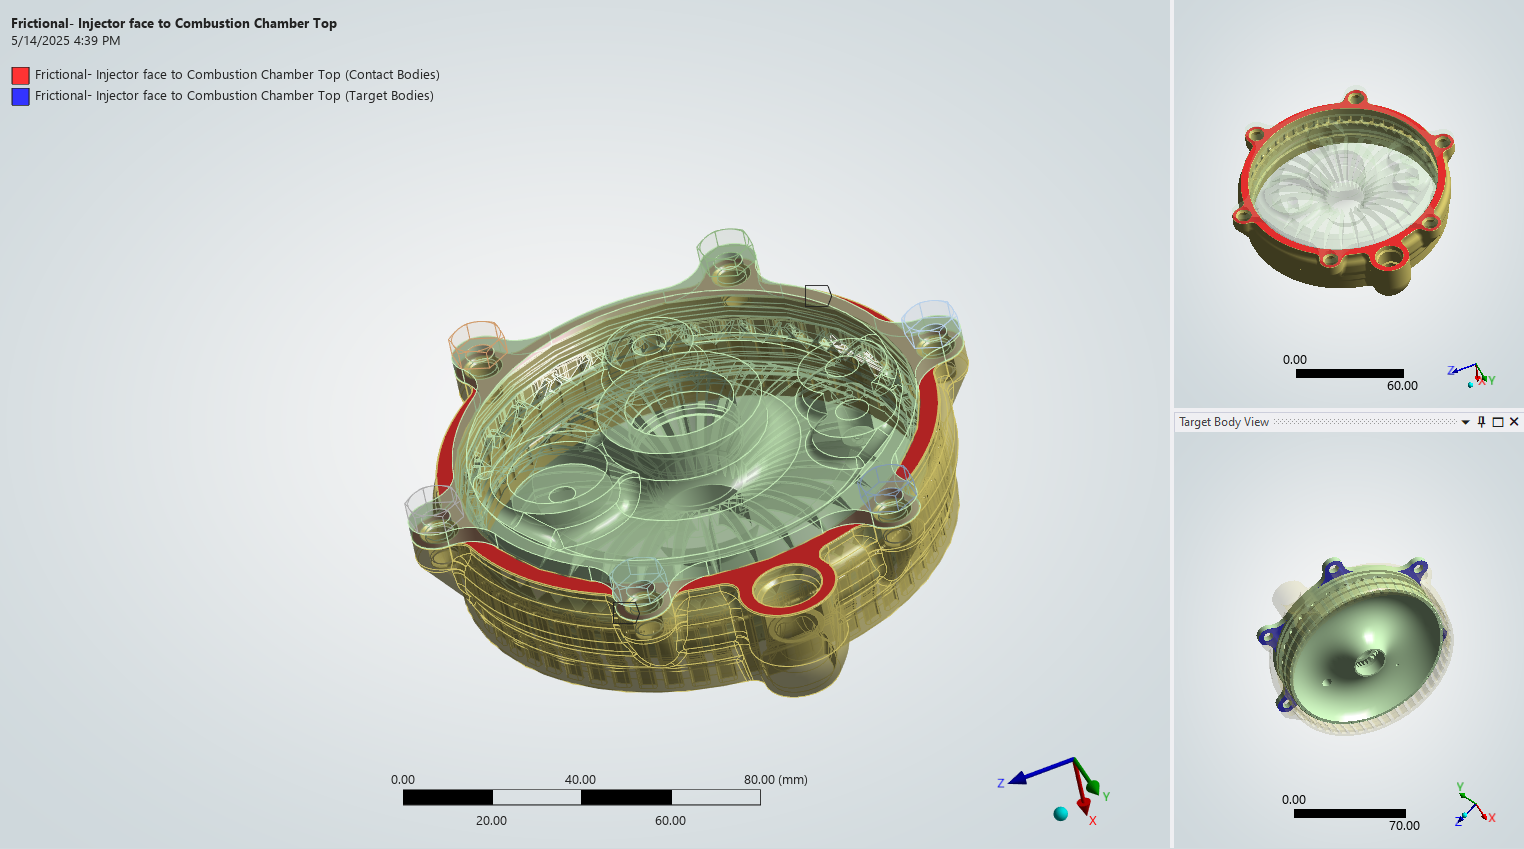
\includegraphics[width=1\linewidth]{Images/Injector Face to Combustion Chamber Top.png}
    \caption{Injector Face to Combustion Chamber Top}
    \label{fig:Injector Face to Combustion Chamber Top}
\end{figure}
The contact between the injector face to combustion chamber top is modeled as frictional, as these surfaces will be clamped together with no lubricant. 
\begin{figure}
    \centering
    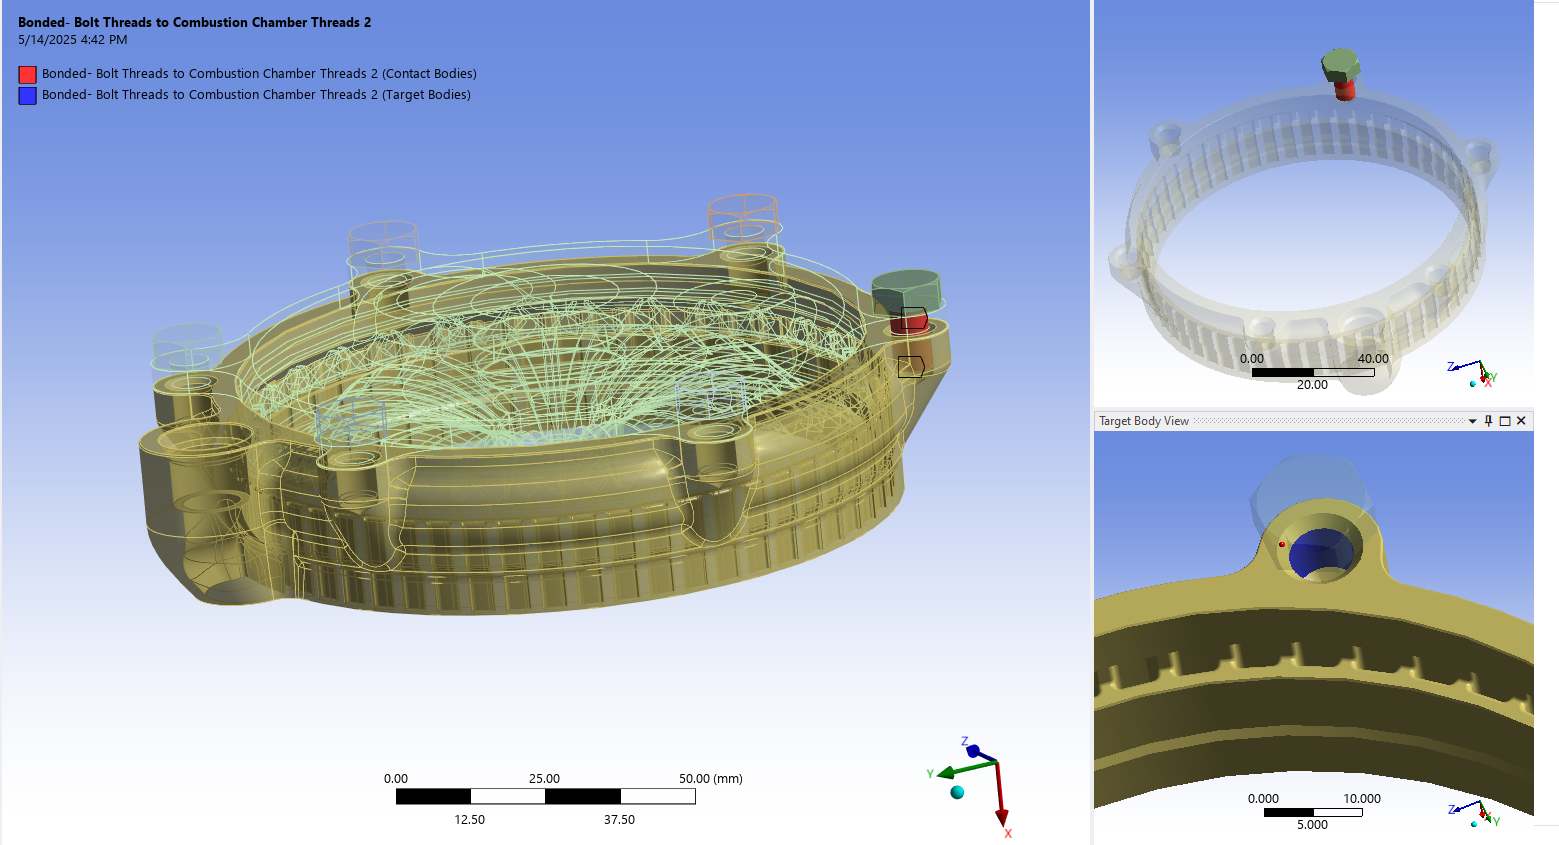
\includegraphics[width=1\linewidth]{Images/Bonded Bolt Threads to Combustion Chamber Threads.png}
    \caption{Bonded Bolt Threads to Combustion Chamber Threads}
    \label{fig:Bonded Bolt Threads to Combustion Chamber Threads}
\end{figure}
The Bolt Threads are modeled as bonded to the combustion chamber threads. This is an appropriate contact to approximate the relationship between the male thread and the female thread. 

\begin{figure}
    \centering
    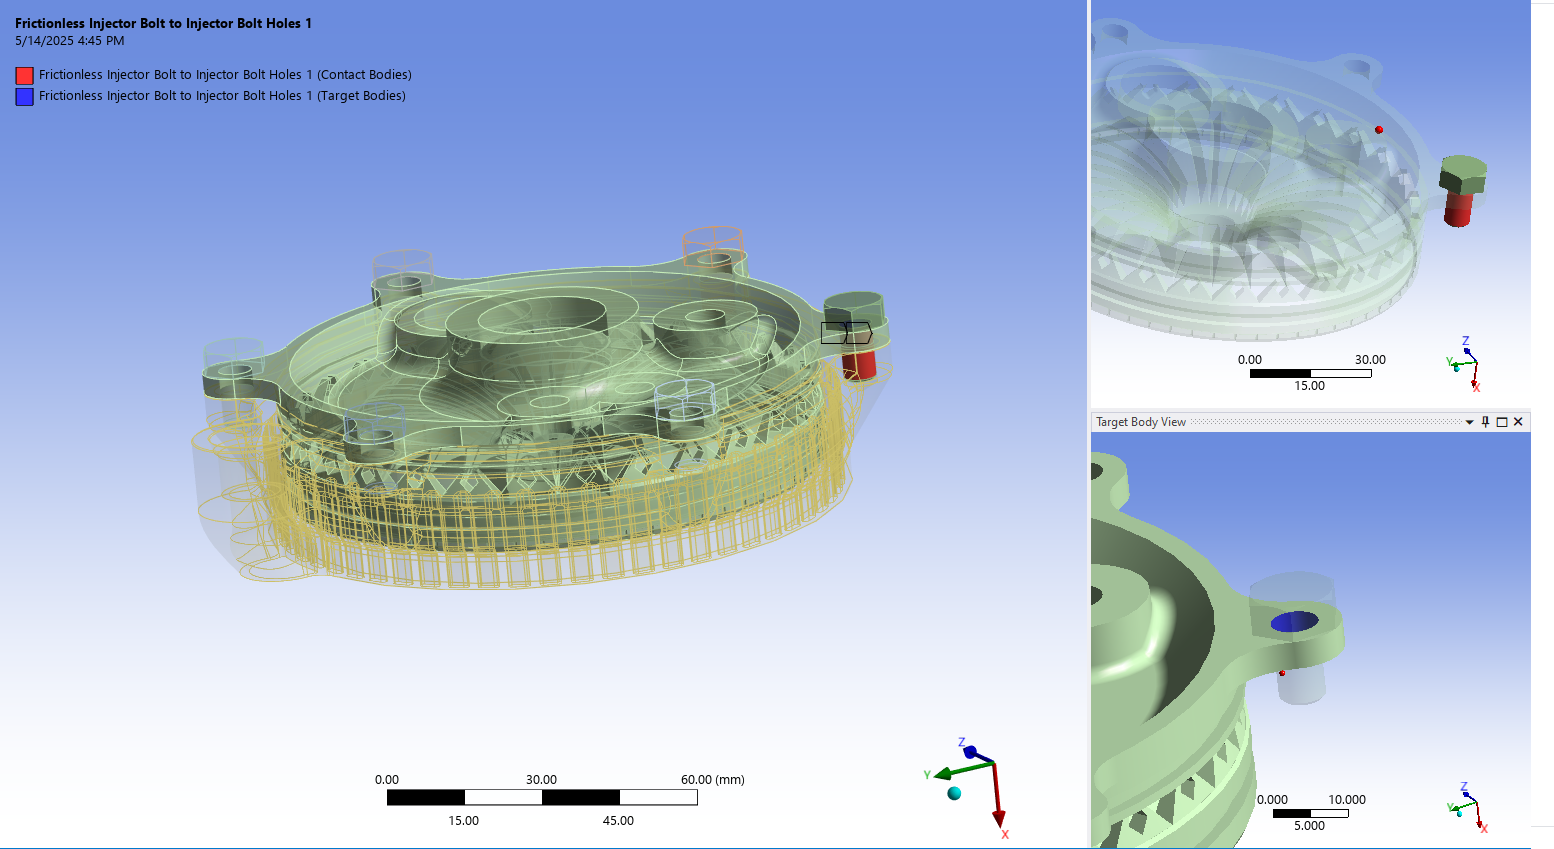
\includegraphics[width=1\linewidth]{Images/Frictionless Injector Bolt to Injector Bolt Holes.png}
    \caption{Frictionless Bolt Shank to Injector Clearance Holes}
    \label{fig:Frictionless Bolt Shank to Injector Clearance Holes}
\end{figure}
The injector bolts are modeled as a frictionless contact with the injector through holes. These surfaces should not come into contact with each other unless the joint is slipping. 

\begin{figure}
    \centering
    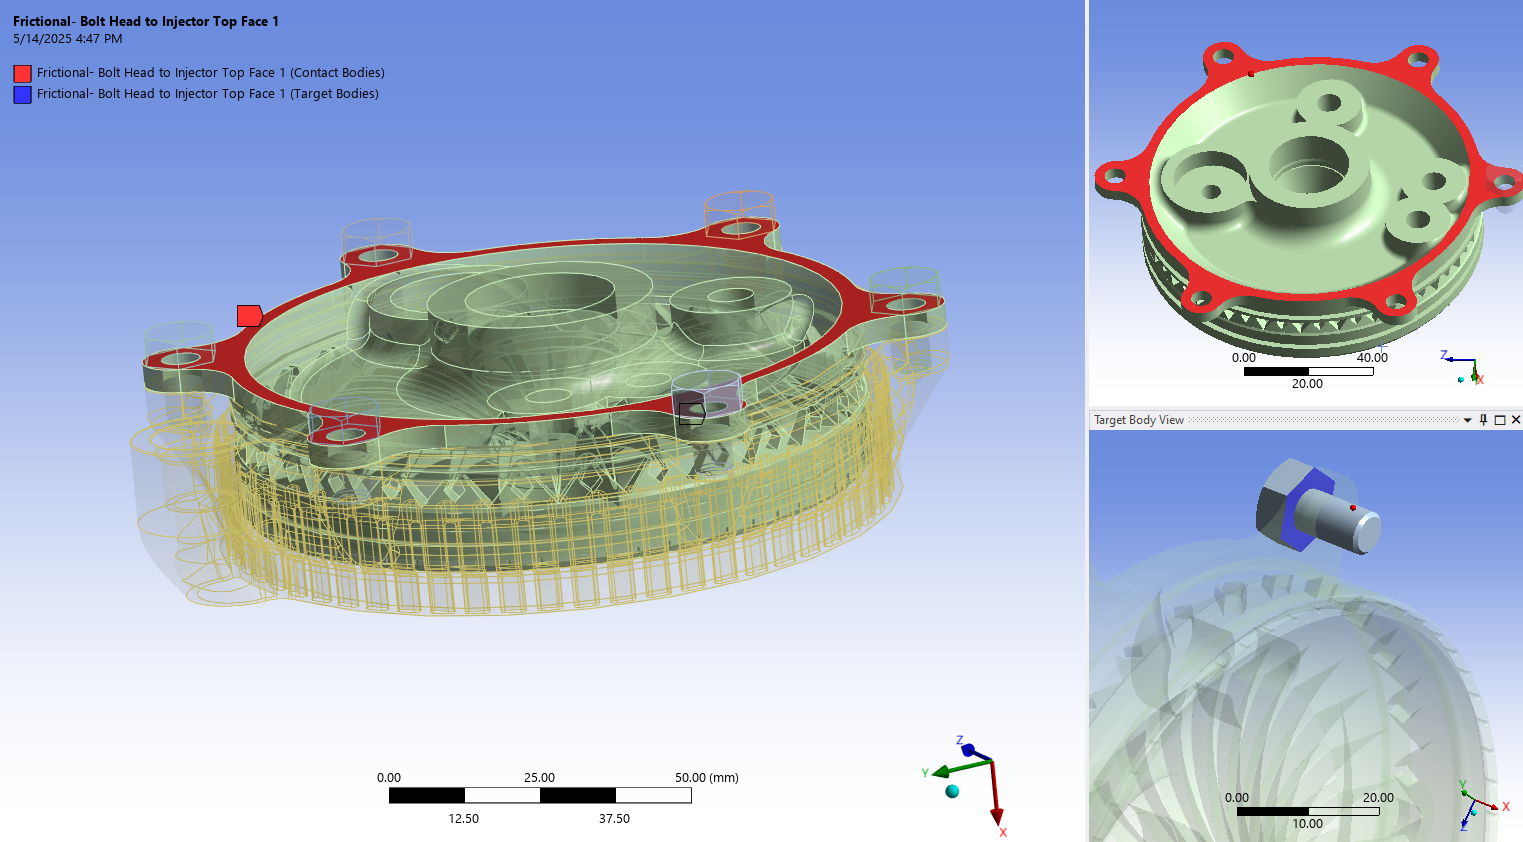
\includegraphics[width=1\linewidth]{Images/Bolt Heat to Injector Top Face.png}
    \caption{Bolt Head to Injector Top Face}
    \label{fig:Bolt Head to Injector Top Face}
\end{figure}
The bolt heads are modeled as frictional contacts with the top face of the injector. These surfaces will be clamped together by the preload on the bolt. The friction factor is modeled to be around 0.2, as expected with lubricated metal to metal surfaces.  A more accurate friction factor can be found through online lookup tables. 
\begin{figure}
    \centering
    \includegraphics[width=1\linewidth]{Images/Supports.png}
    \caption{Supports}
    \label{fig:Supports}
\end{figure}
The injector is constrained with a fixed support on the central port. This is a reasonable constraint, as this part of the injector is already very stiff, so fixing this face will not significantly affect the stiffness of the rest of the model. 
The sliced breakout model has a frictionless support on the cut plane, which is used as a symmetry boundary condition. The model is not actually symmetric around the cut plane, but it is an accurate approximation when analyzing the top section of the combustion chamber. 

\subsection{Loads}
The yield load factor is 1.5, and the ultimate load factor is 2.0. The load factor method is used rather than analyzing safety factor because there are nonlinear effects that invalidate any simple scaling of results. Multiple pressure load cases were considered:

\begin{enumerate}
    \item \textbf{Fuel Channel Pressure}
    \begin{itemize}
        \item Yield pressure: $1500\,\text{PSI}$ ($10.34\,\text{MPa}$)
        \item Ultimate pressure: $2000\,\text{PSI}$ ($13.74\,\text{MPa}$)
    \end{itemize}
    
    \item \textbf{Combustion Chamber Internal Pressure}
    \begin{itemize}
        \item Yield pressure: $525\,\text{PSI}$ ($3.61\,\text{MPa}$)
        \item Ultimate pressure: $700\,\text{PSI}$ ($4.82\,\text{MPa}$)
    \end{itemize}

    \item \textbf{Thermal Stress}
    \begin{itemize}
        \item Imported thermal loads from RPA 
    \end{itemize}
    \item \textbf{Preload}
    \begin{itemize}
        \item 9000N of preload is applied to each bolt
    \end{itemize}
\end{enumerate}


\subsection{Preload}

The injector is attatched to the chamber body with a bolted joint. The bolted joint in this analysis is modeled with the actual bolt body rather than beams to capture more information about the joint. The bolts must be preloaded such that the joint does not separate when the engine is at operating pressure. The bolts must provide enough clamping force to overcome the force of the chamber pressure pushing on the injector. 
\begin{align}
A            &= 13.5~\text{in}^2 \\[2pt]
P            &= 350~\text{psi}                                          \\[6pt]
F_{\text{total}}
             &= P \, A
               = 350~
               \frac{\text{lbf}}{\text{in}^2}
               \times 13.5~\text{in}^2
               = 4\,725~\text{lbf}                                       \\[2pt]
             &= 4\,725~\text{lbf}\,
                \bigl(4.44822~\tfrac{\text{N}}{\text{lbf}}\bigr)
               \approx 2.10\times10^{4}~\text{N}                         \\[12pt]
n_{\text{bolts}}
             &= 6                                                      \\[6pt]
F_{\text{per~bolt}}
             &= \frac{F_{\text{total}}}{n_{\text{bolts}}}
               = \frac{2.10\times10^{4}~\text{N}}{6}
               \approx 3.50\times10^{3}~\text{N}                        \\[2pt]
             &\approx 786~\text{lbf}
\end{align}
Each bolt must provide at least 786 lbf of clamping force. This value is inputted into the bolted joint spreadsheet, based on NASA STD\_5020. 

Because there is a Helicoil, we have to do the bolted joint calculations in several steps as shown in the above figures. The first step is calculating how much preload is required to prevent joint separation. The pressure force is applied as the Tension limit load. There should be no shear load in this joint, but 100 lbf is used as a placeholder value. Next, the joint dimensions are inputted. The Helicoil length is 1.0D which means it is 0.25. This value is used for the engagement depth. Next, the material is inputted, and the insert is stainless steel. The preload is adjusted such that the joint has a positive margin for separation. This is a "separation critical joint" so there is already a 1.4FOS applied to the joint separation. 

 \begin{figure}
     \centering
     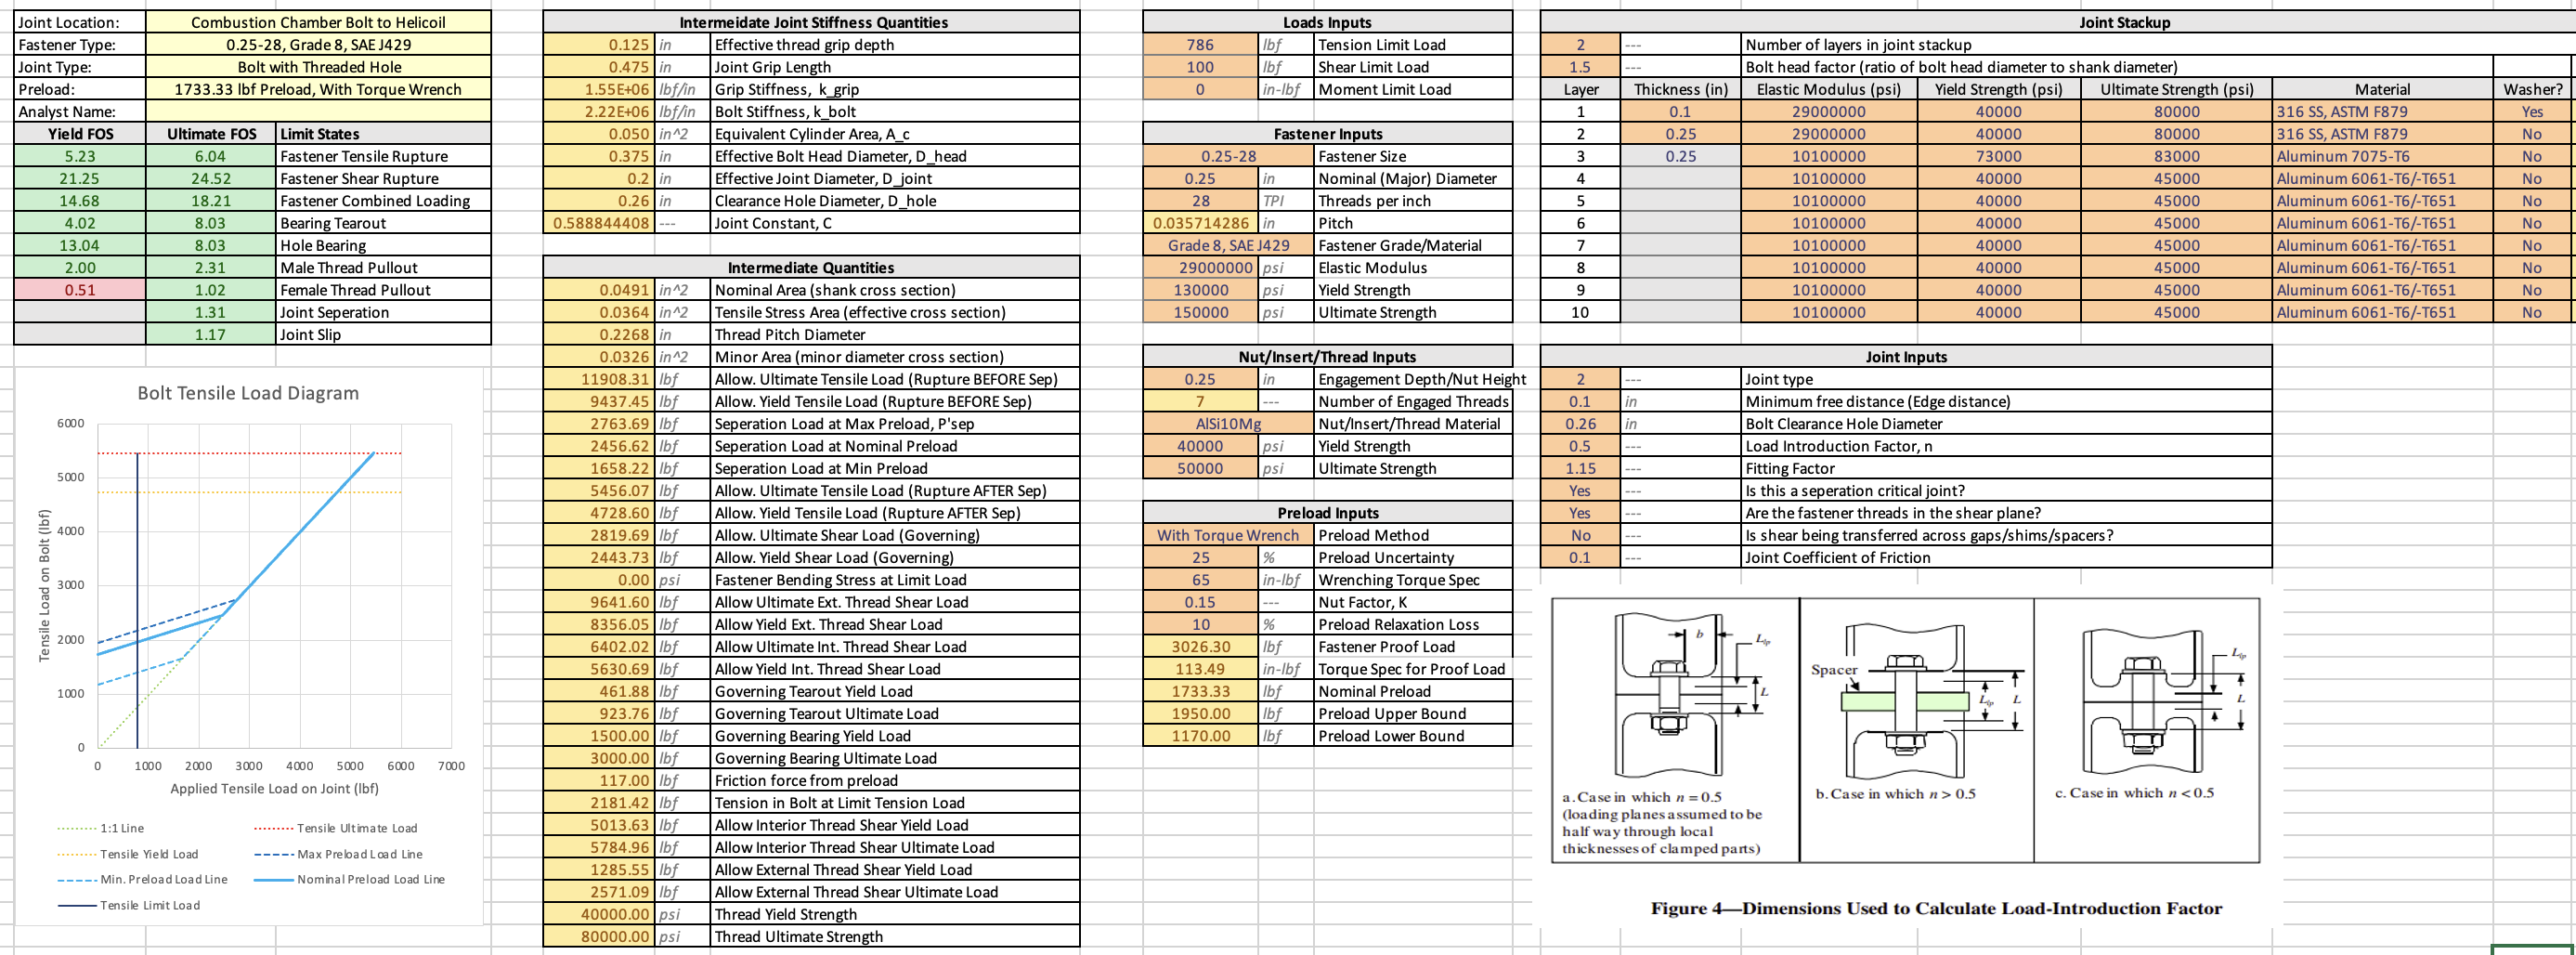
\includegraphics[width=1\linewidth]{Combustion Chamber Bolt to Helicoil.png}
     \caption{Combustion Chamber Bolt to Helicoil}
     \label{fig:Combustion Chamber Bolt to Helicoil}
 \end{figure}
The negative margin on yield is ignored, as it is local non detrimental yielding of the Helicoil and the fatigue life of this engine is not relevant. 

Next, the combustion chamber to Helicoil bolted joint is analyzed in a similar manner. Joint separation is not relevant in this calculation because we are only considering the interaction between the Helicoil and the chamber. 

 \begin{figure}
     \centering
     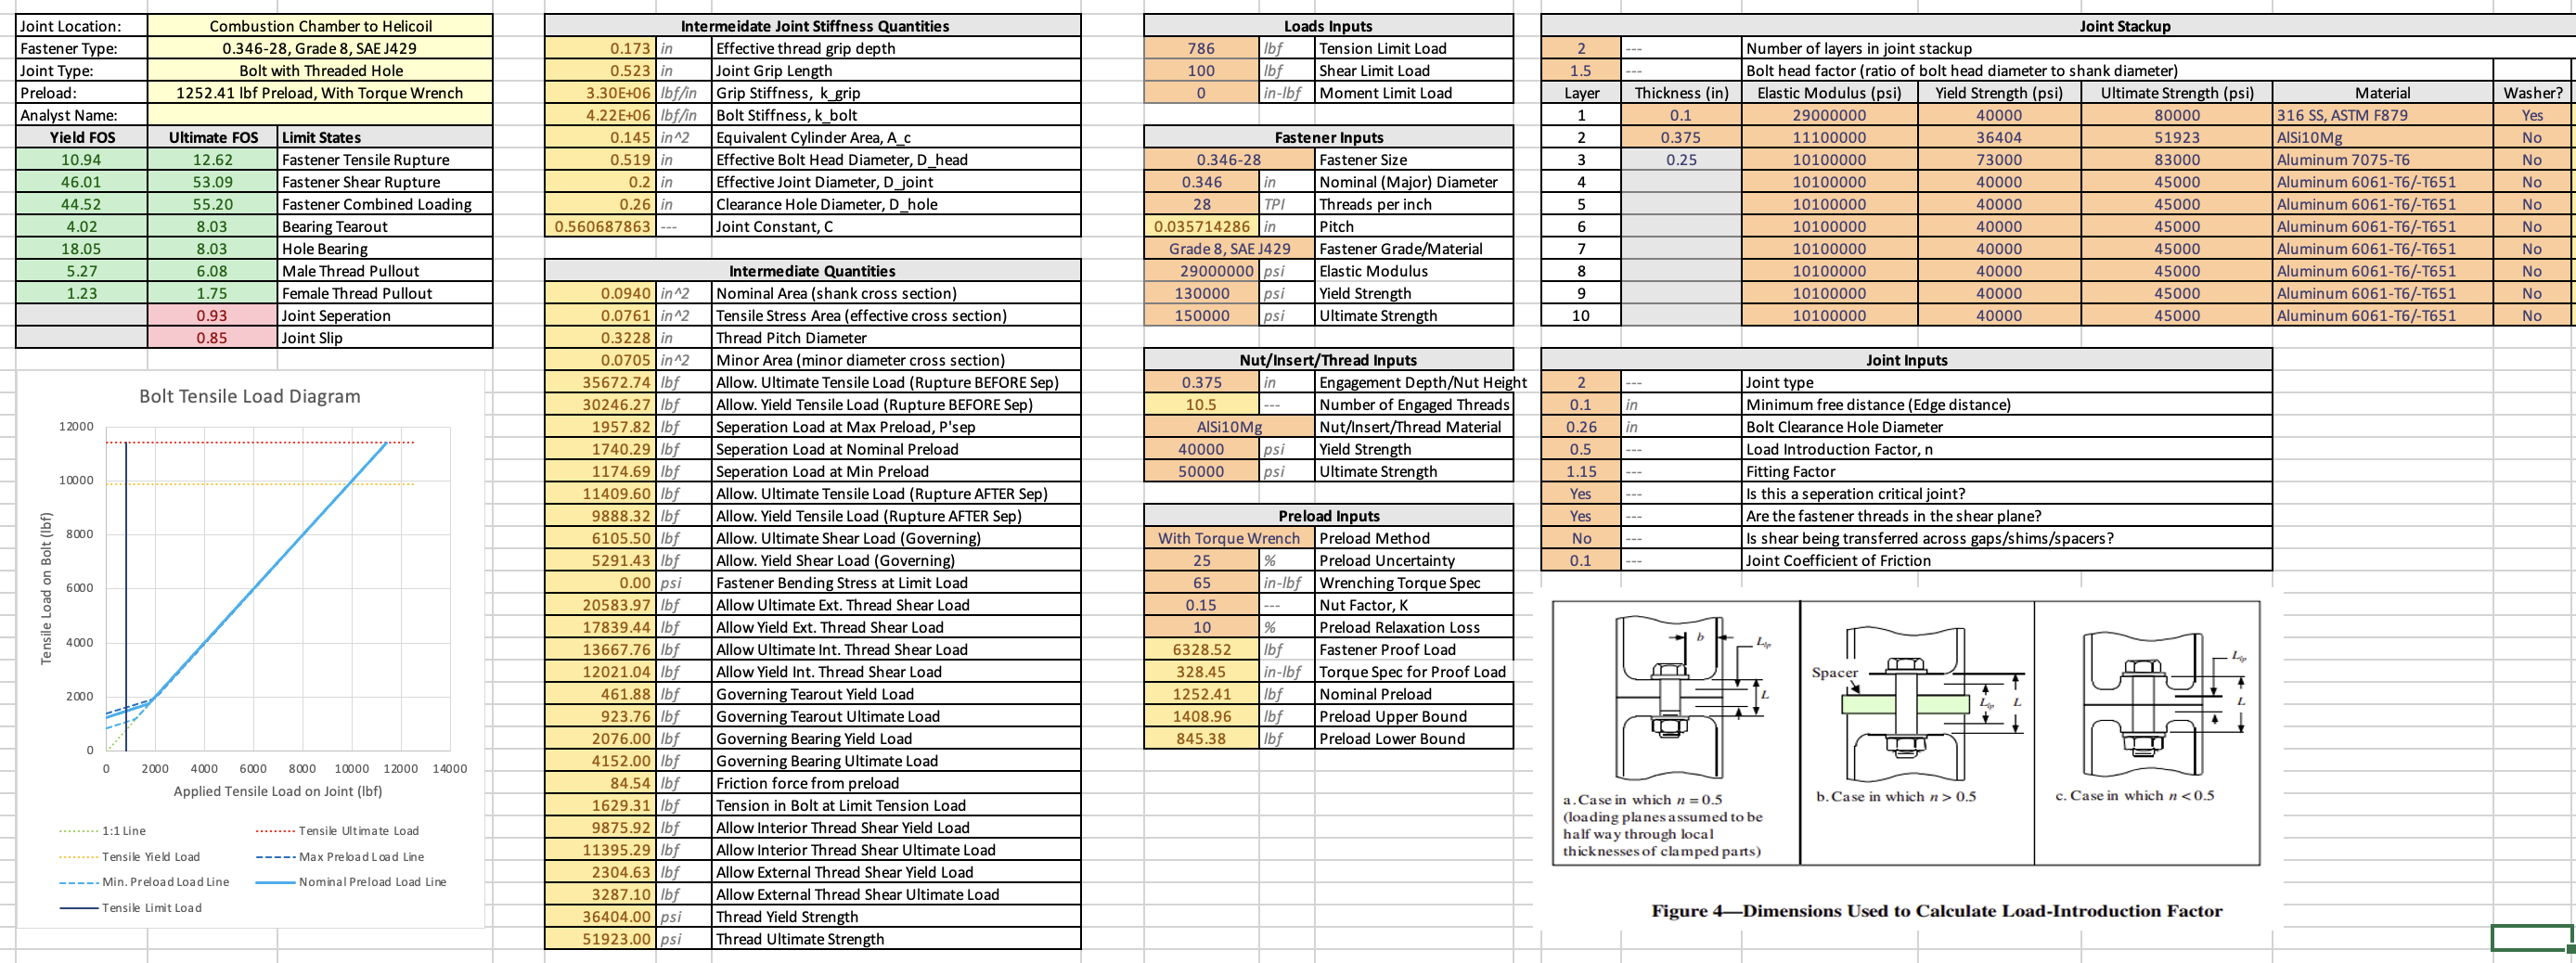
\includegraphics[width=1\linewidth]{Images/Combustion Chamber to Helicoil.png}
     \caption{Combustion Chamber to Helicoil}
     \label{fig:Combustion Chamber to Helicoil}
 \end{figure}
This joint passes. The 1/4 28 fastener should be tightened to 65 in-lbs for a nominal preload of 1733lbf. The preload upper bound is 1950 lbf , which equals roughly 9000N, which is what was used for the preload value in Ansys. 

 


Pressure loads are applied to internal faces as shown below. Fuel pressure is applied to all surfaces that are in contact with fuel, and chamber pressure is applied to all internal faces that are in contact with chamber gases. The same loads are applied to all models as seen in Figure \ref{fig:CombinedSetup}.
\begin{figure}
    \centering
    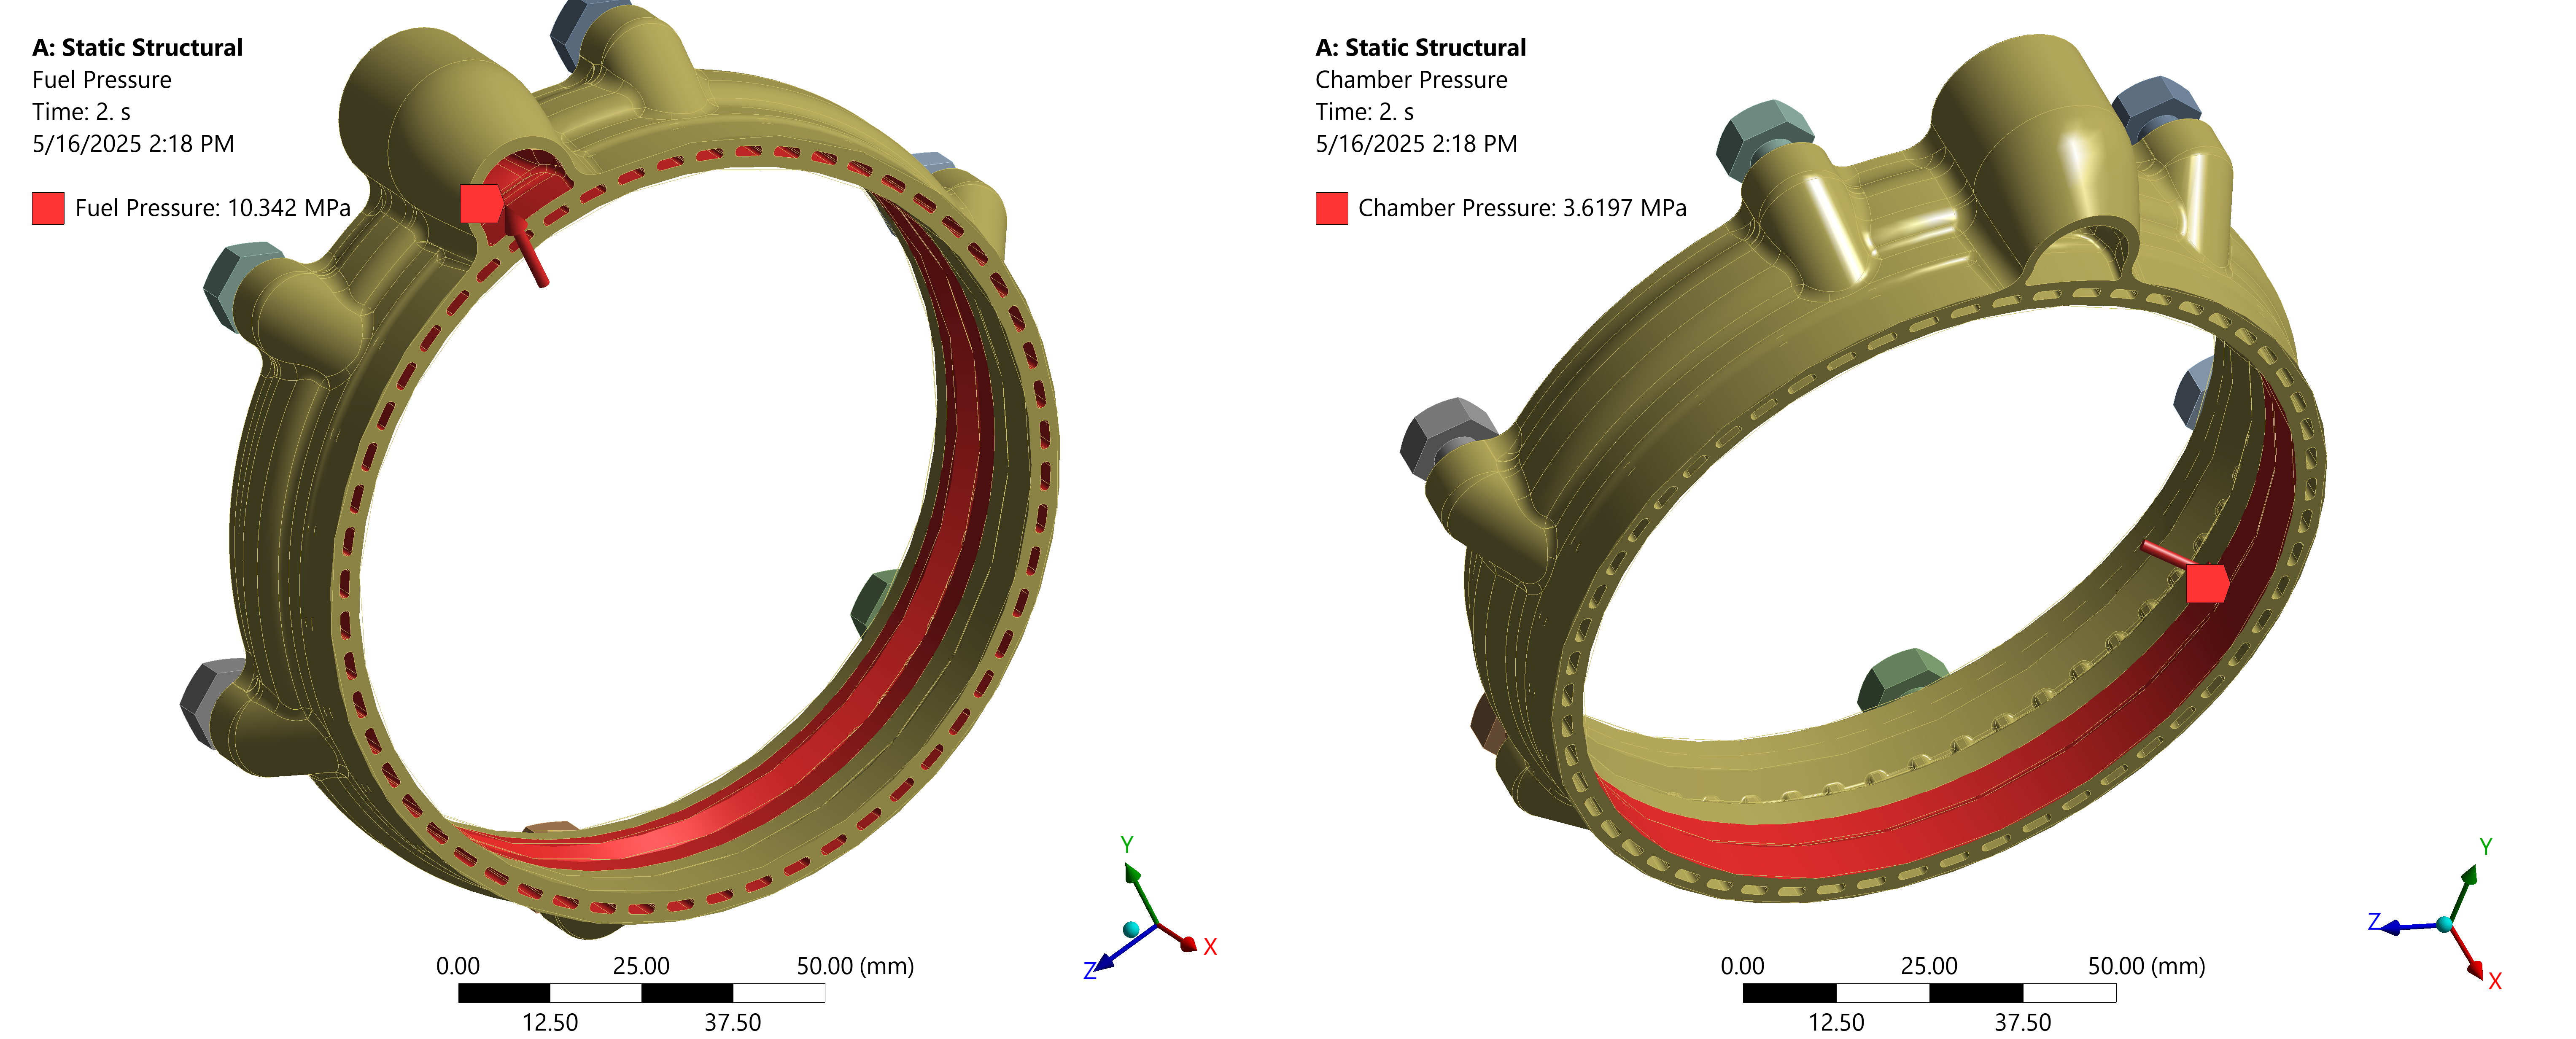
\includegraphics[width=1\linewidth]{Images/Pressure Loads.png}
    \caption{Pressure Loads}
    \label{fig:Pressure Loads}
\end{figure}
\subsection{Thermal-Structural Coupling}

The temperature results from RPA as seen in Figure \ref{fig:aluminum_temp_profile} were imported into Ansys to evaluate thermal stresses:
\begin{enumerate}
    \item Temperature data was exported from RPA into CSV format with axial location and wall temperature
    \item A steady-state thermal analysis module was created in Mechanical
    \item Imported load data was applied to the appropriate surfaces
    \item Temperature distributions were mapped to the structural model
\end{enumerate}
\begin{figure}
    \centering
    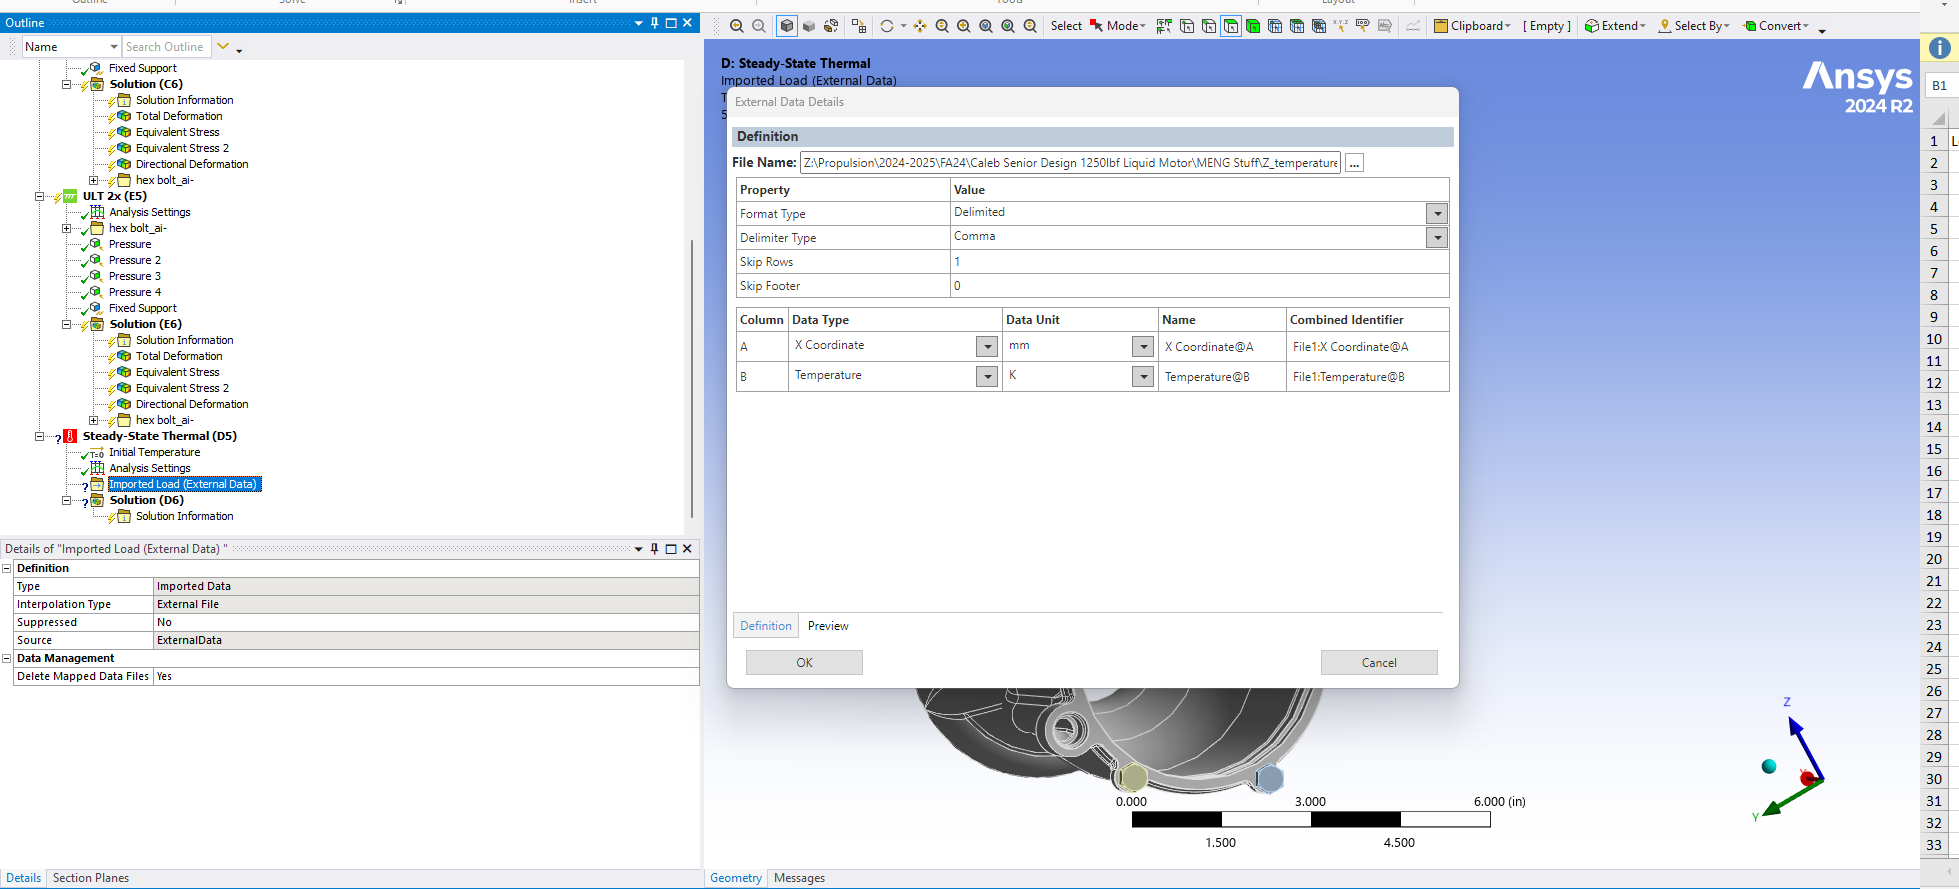
\includegraphics[width=1\linewidth]{Images/ThermalCouplingsetup.png}
    \caption{Thermal Coupling Setup}
    \label{fig:Thermal Coupling Setup}
\end{figure}
The wall temperatures (TWG) are mapped to the inner combustion chamber faces, while the cool side temperatures (TWC) are mapped to the inside of the cooling channels. 
\begin{figure}
    \centering
    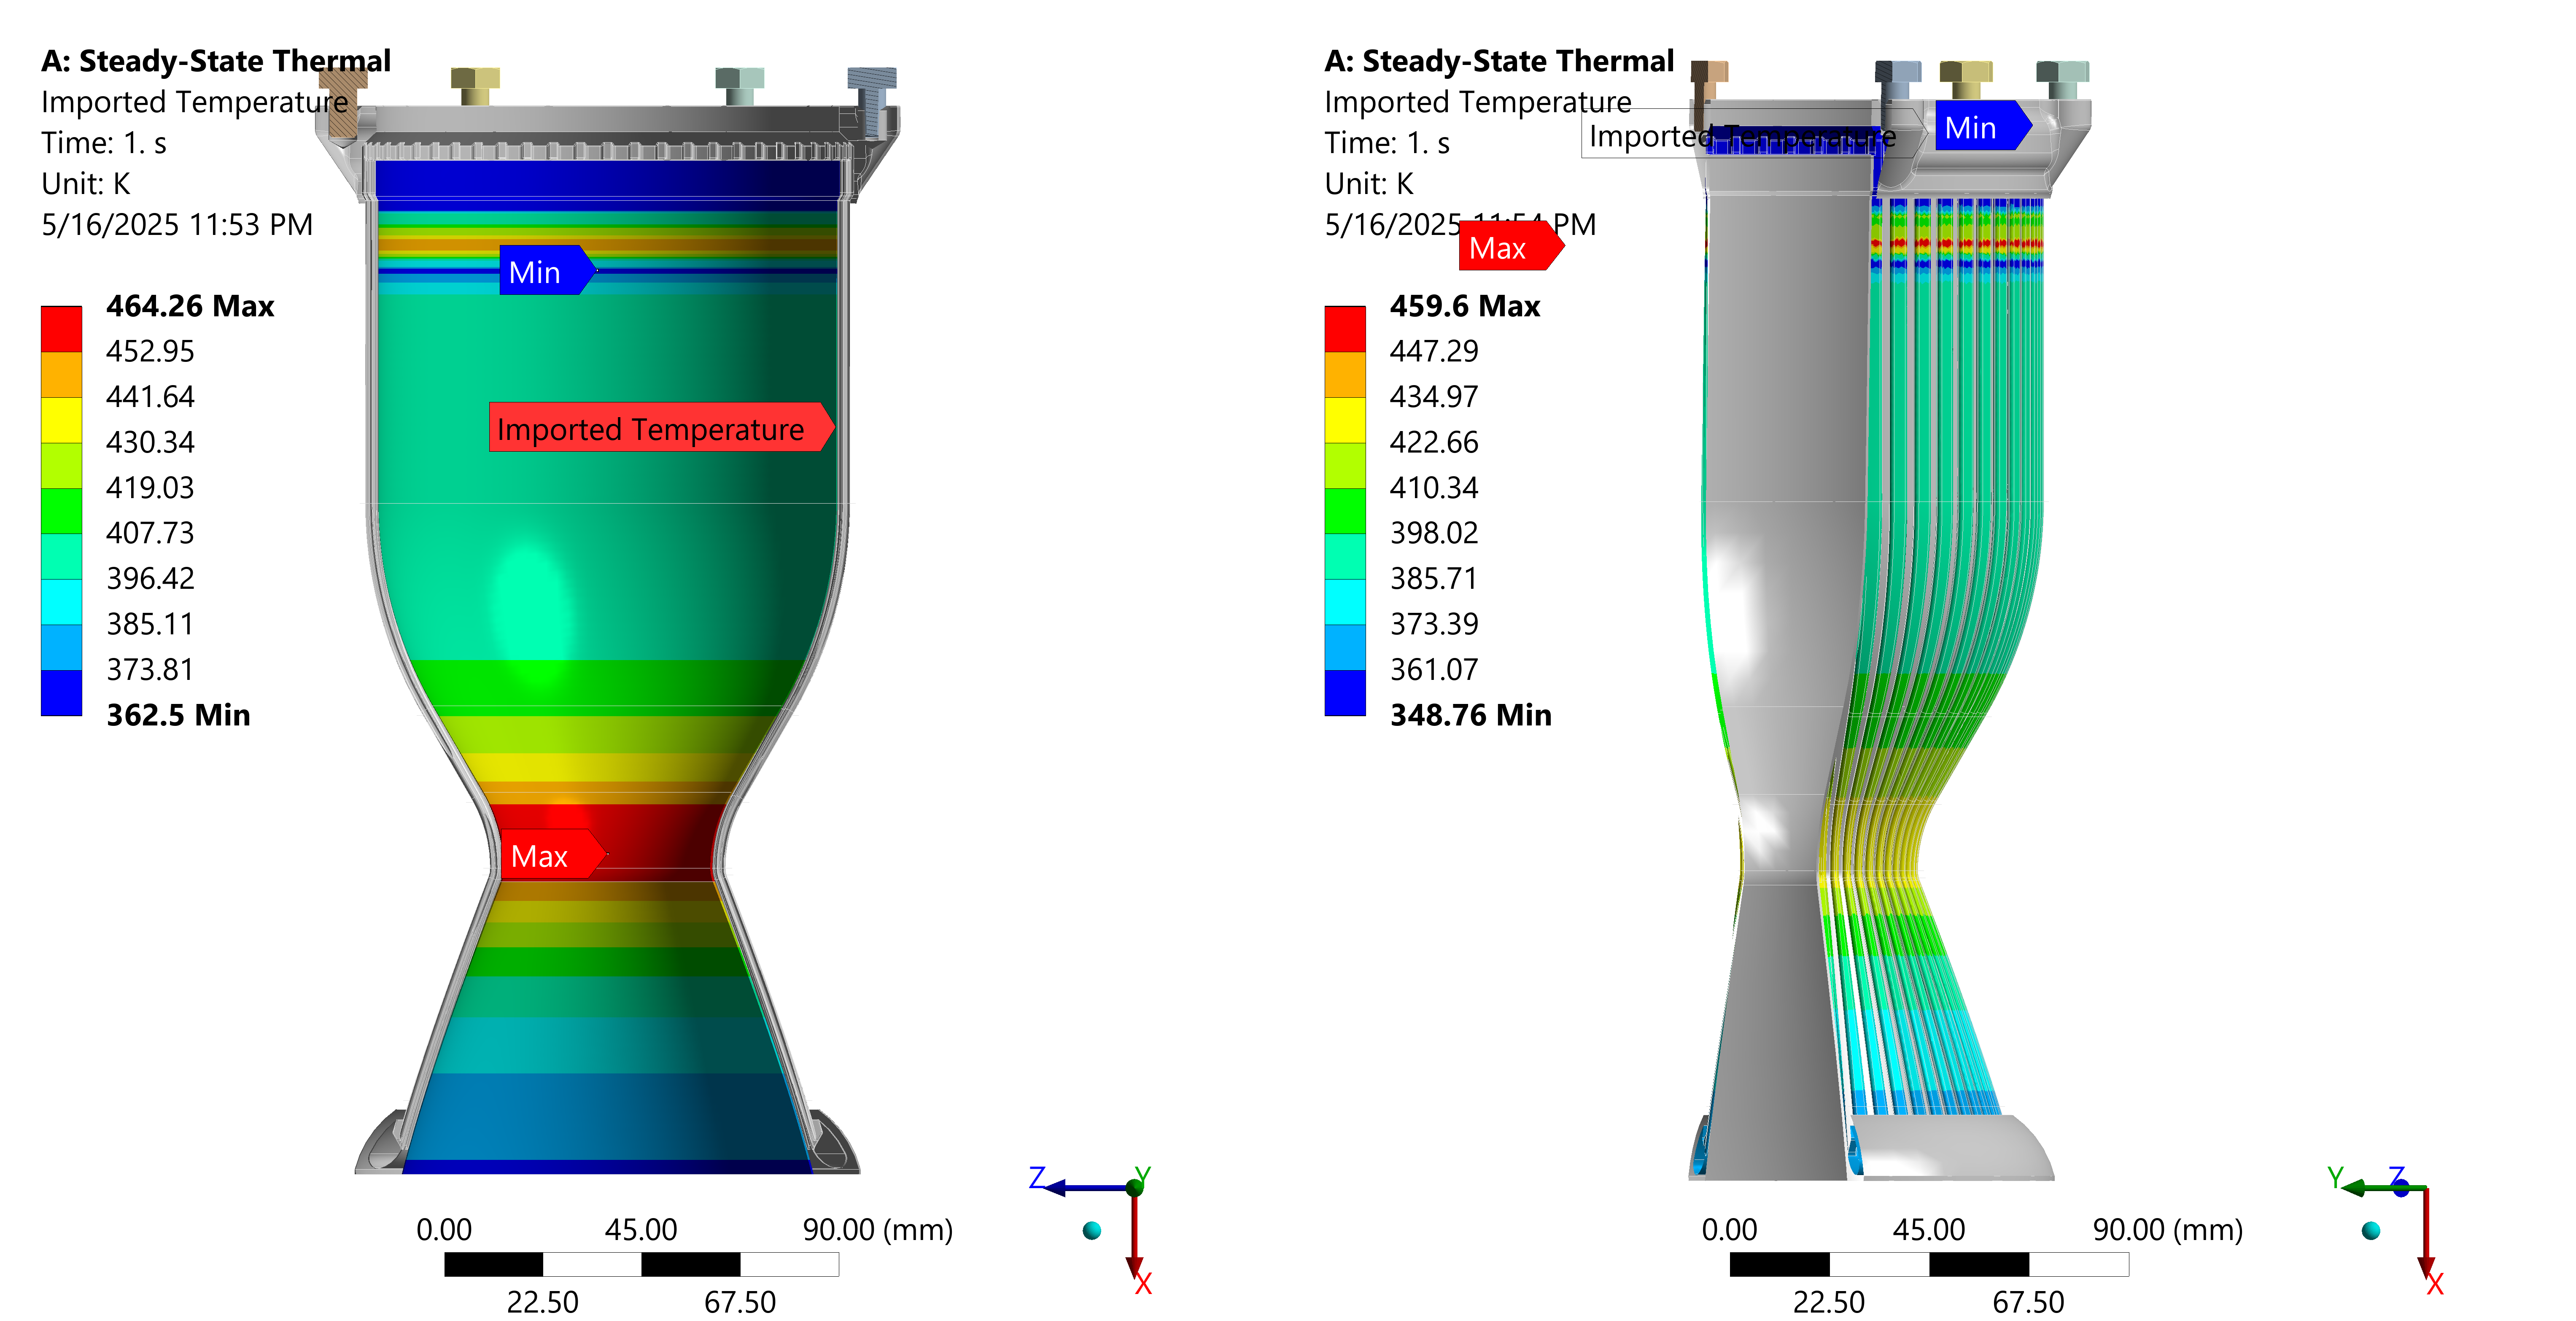
\includegraphics[width=1\linewidth]{Images/Raw RPA Imported Temperatures.png}
    \caption{Raw RPA Imported Temperatures}
    \label{fig:Raw RPA Imported Temperatures}
\end{figure}
The spiky initial temperature fluctuations observed in some results were identified as numerical instabilities related to the Bartz singularity, where the convective heat transfer coefficient yielded ``nan'' values at positions below $20\,\text{mm}$. For analysis purposes, these areas were smoothed using stable temperature values from adjacent regions.
\begin{figure}
    \centering
    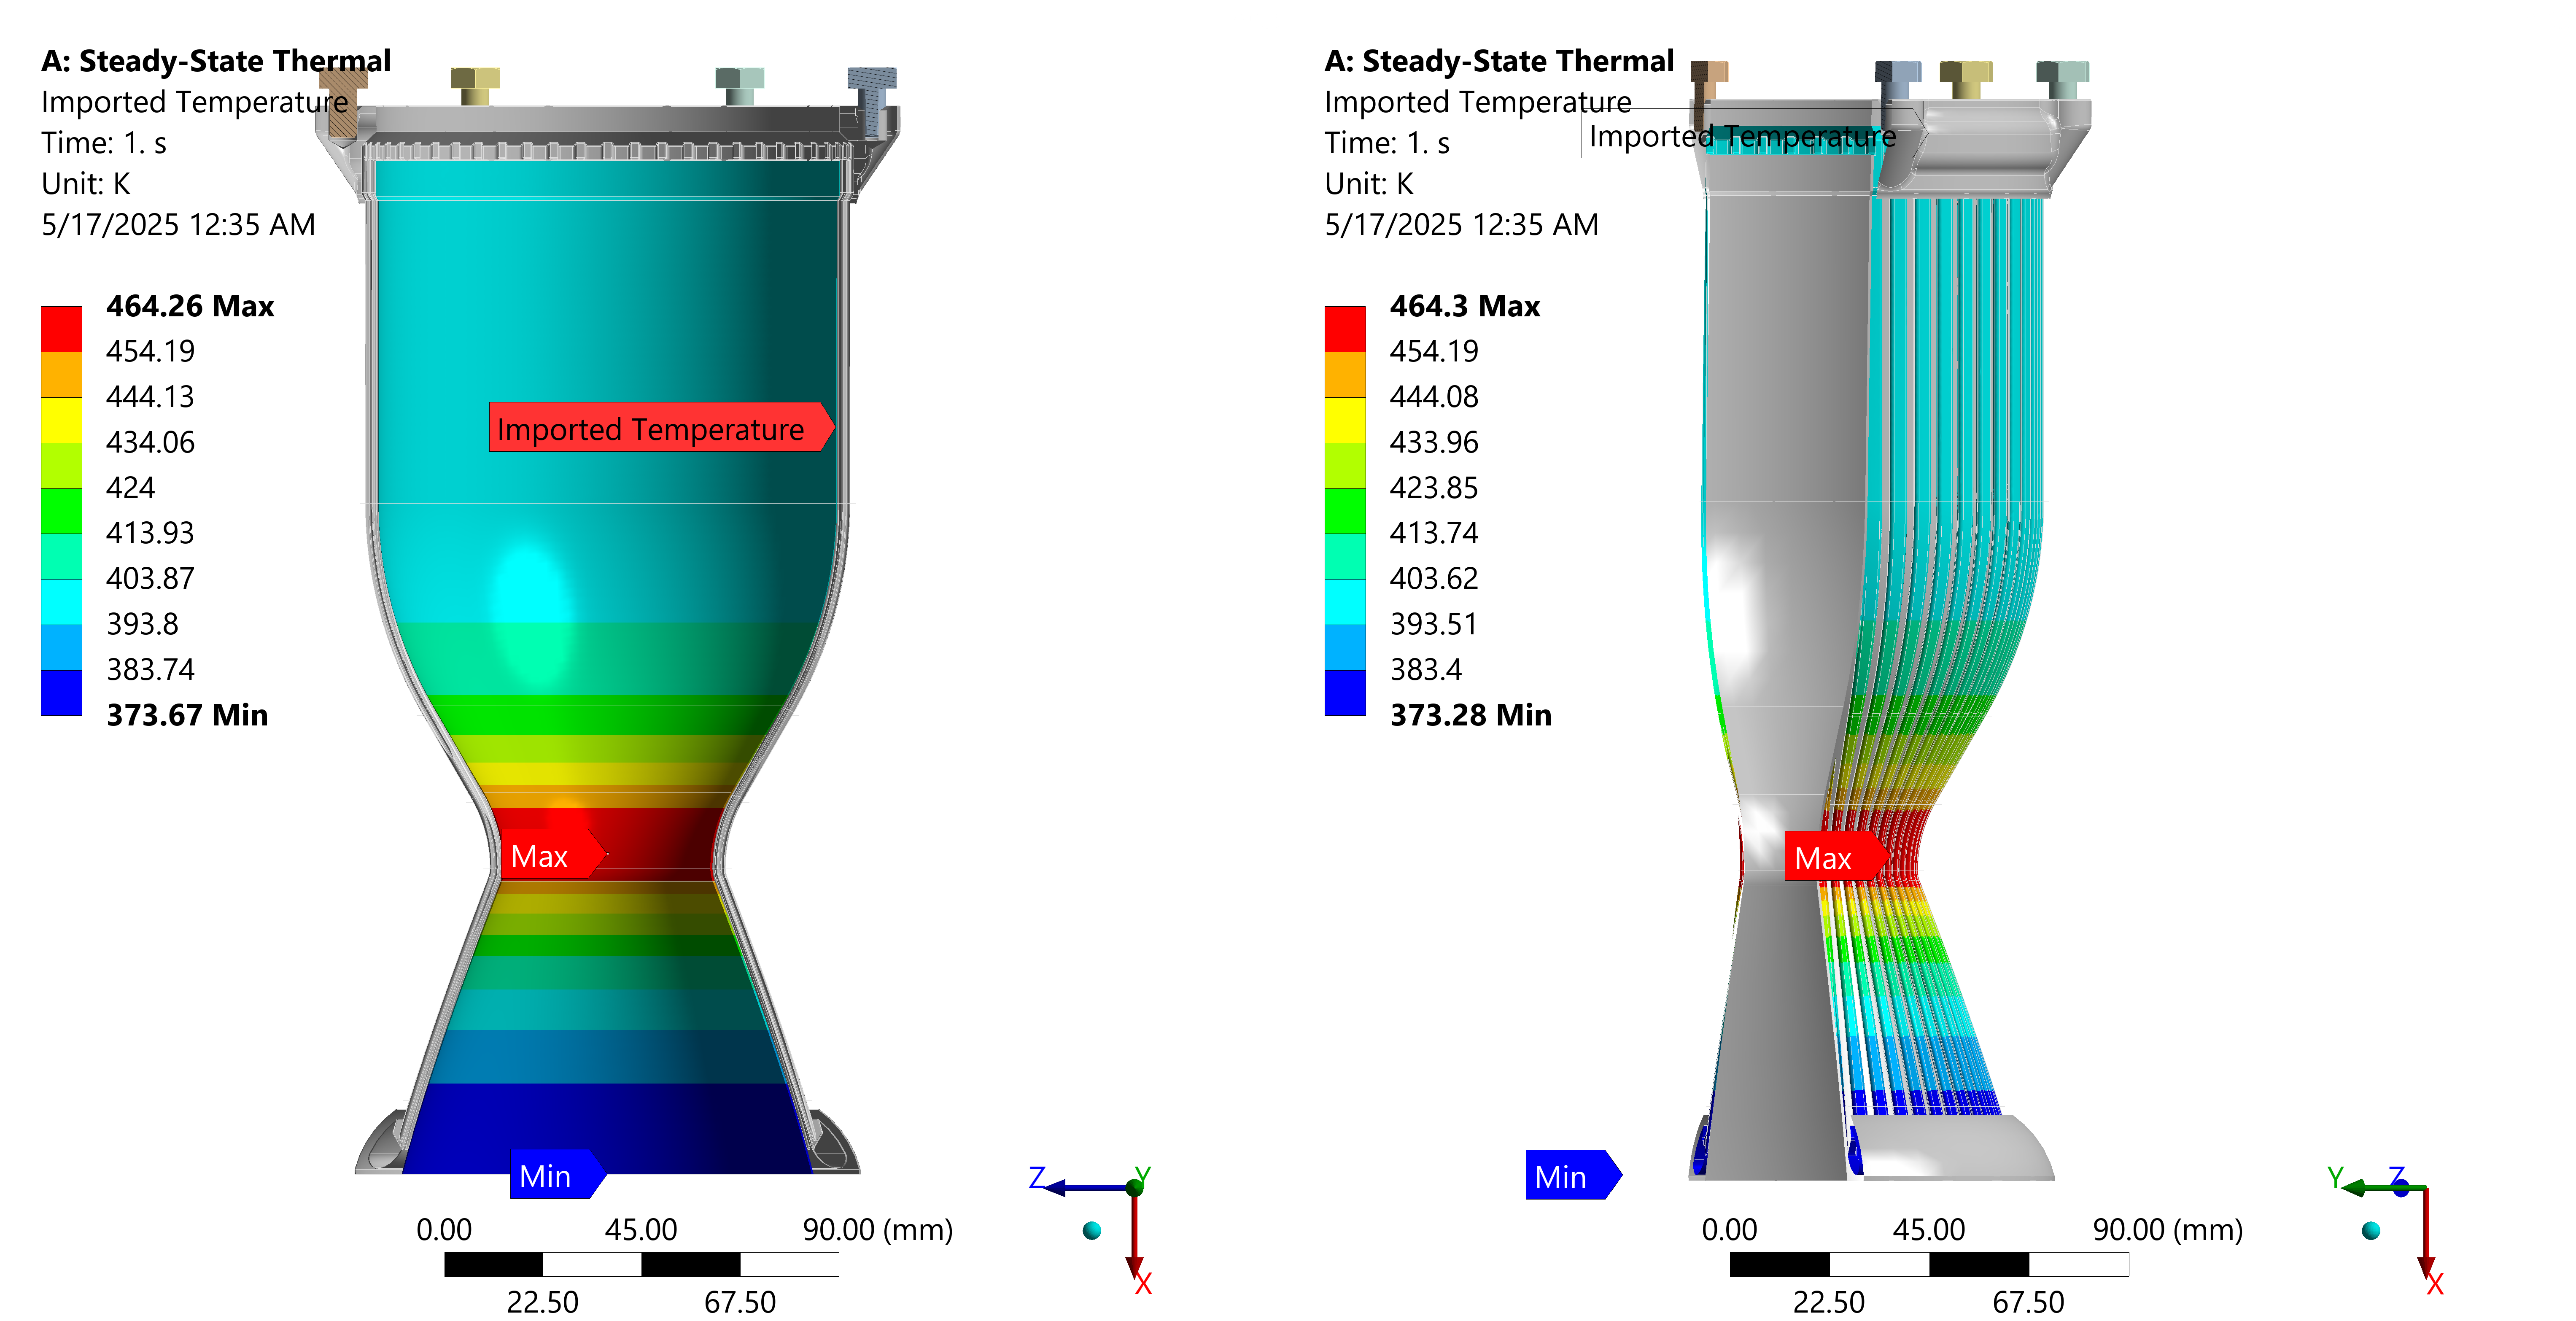
\includegraphics[width=1\linewidth]{Images/Imported Temperatures.png}
    \caption{Smoothed RPA Imported Temperatures}
    \label{fig:Smoothed RPA Imported Temperatures}
\end{figure}

The steady-state thermal analysis yielded wall temperatures reaching a maximum of approximately $465\,\text{K}$ at the throat as expected. The thermal gradient is captured accurately, which will serve to model thermal stresses in areas with high temperature differentials.  
\begin{figure}
    \centering
    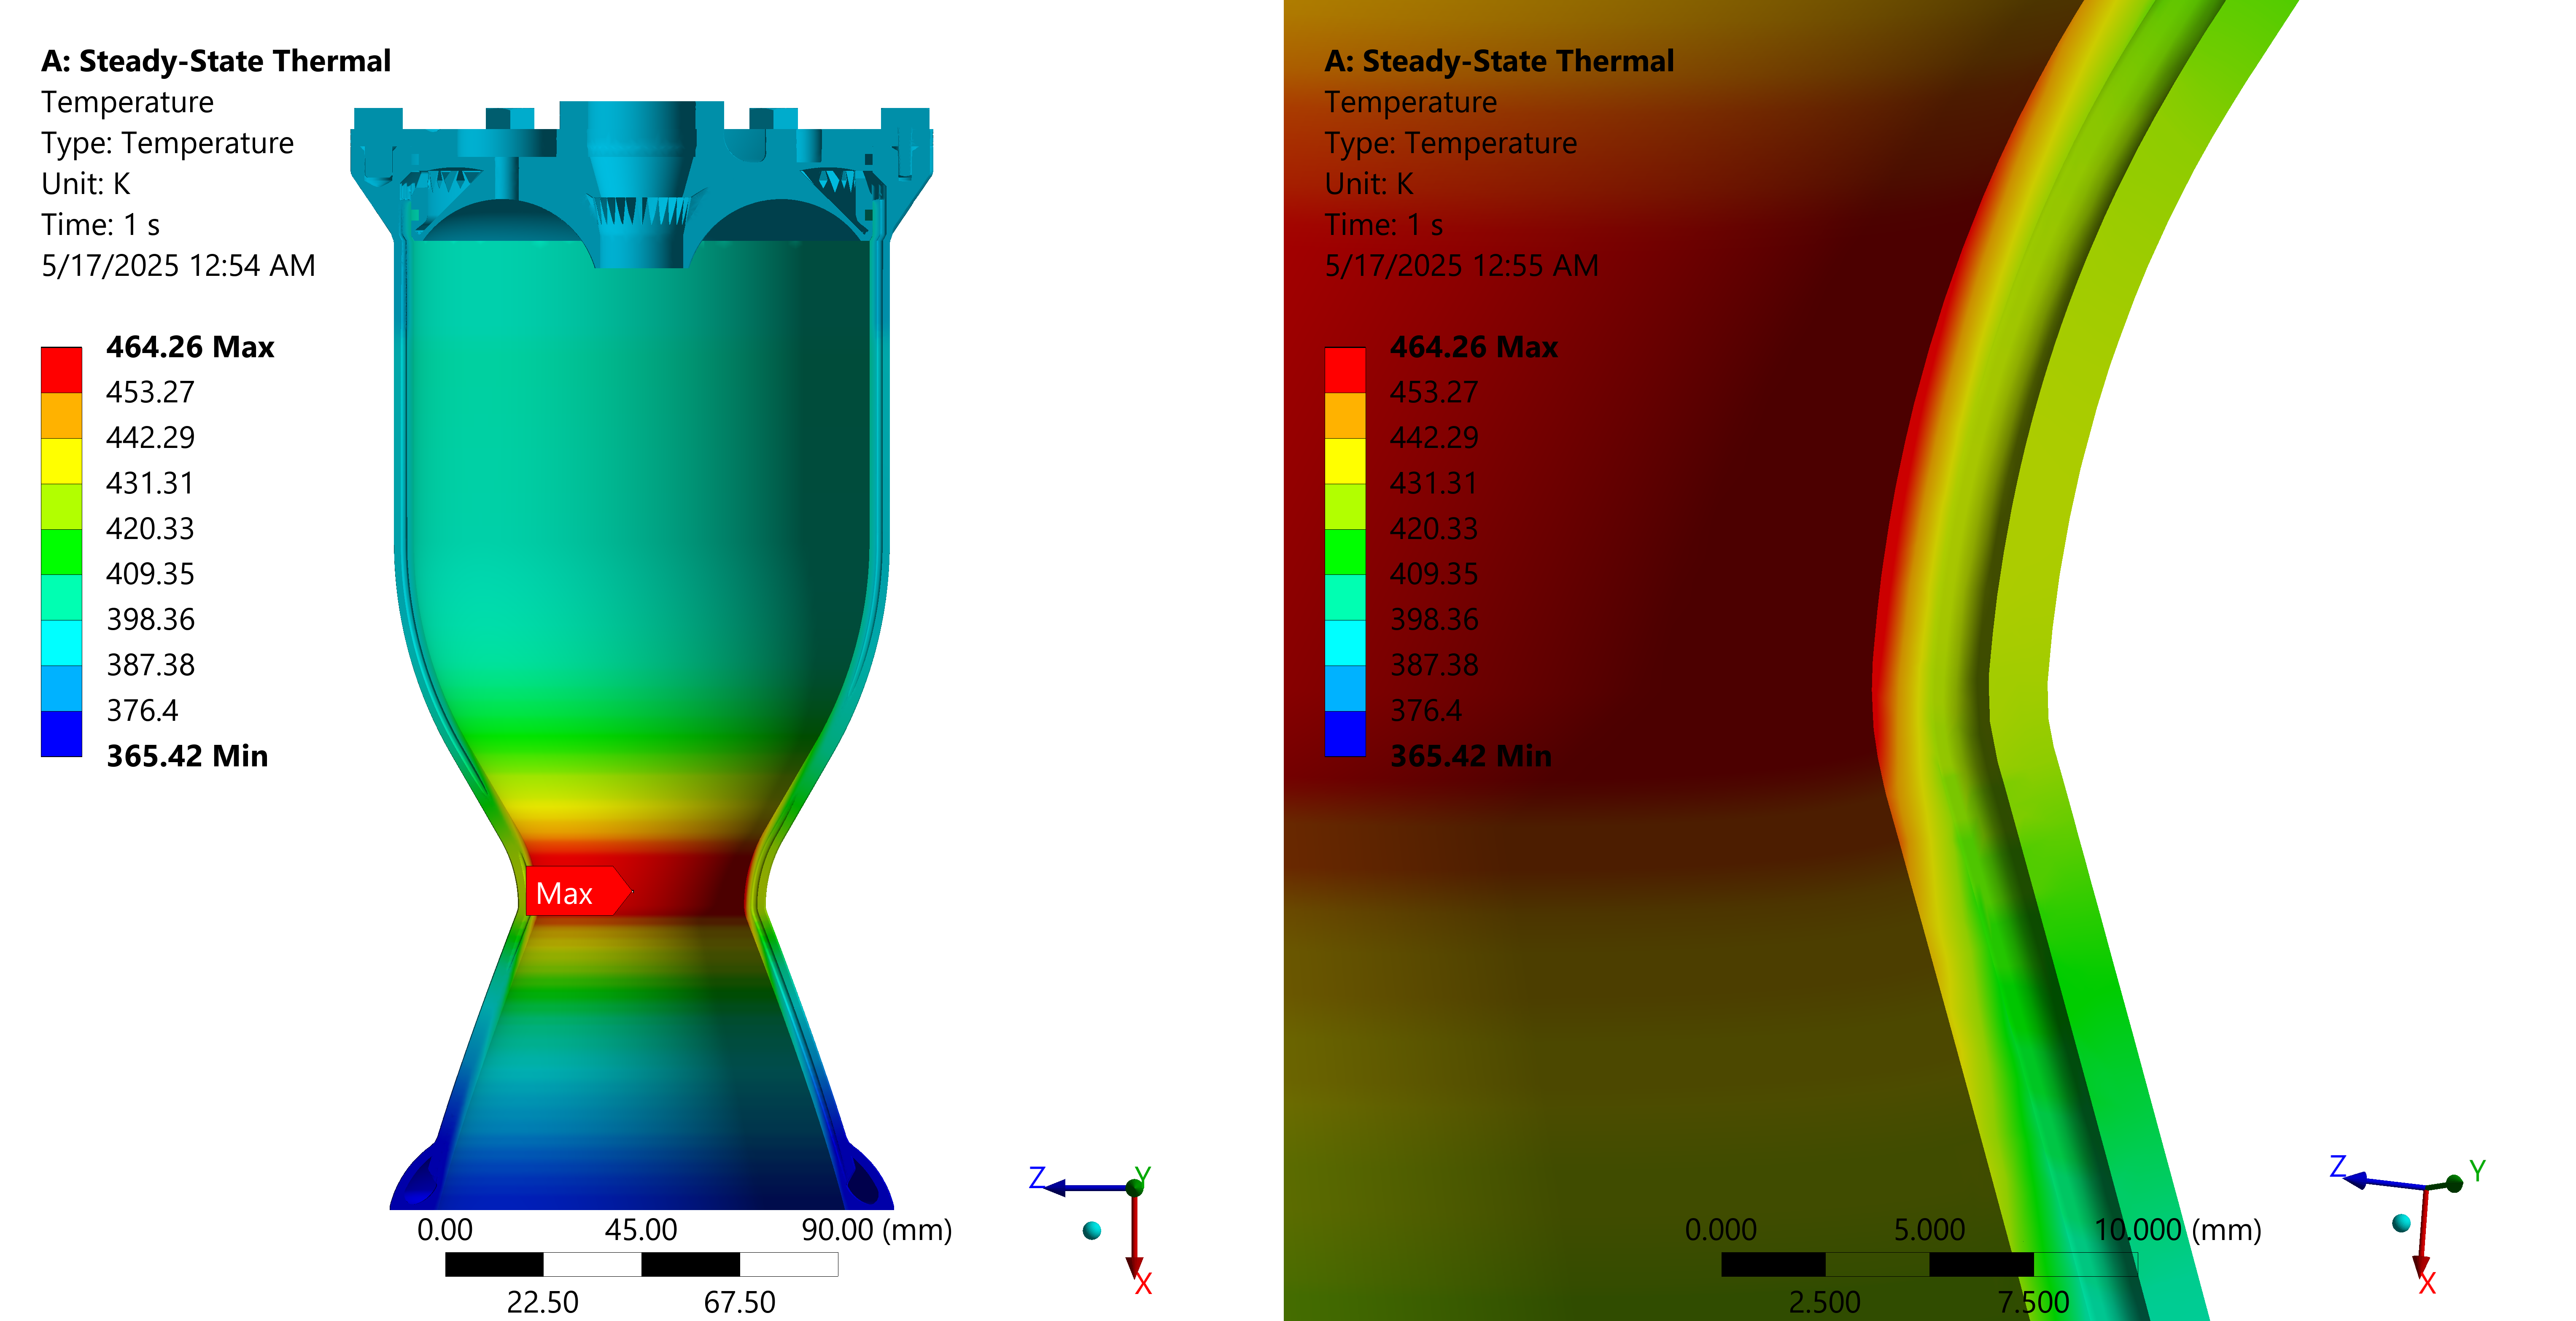
\includegraphics[width=1\linewidth]{Images/Steady-State Temperature.png}
    \caption{Steady-State Temperature}
    \label{fig:Steady-State Temperature}
\end{figure}

While these results provide good insight into operational temperatures, they do not capture the initial transient conditions where thermal stresses would be significantly higher. Additionally, the model does not incorporate the complete heat transfer mechanisms present in the actual engine. However, these transient effects are expected to be balanced out by the fact that AlSi10Mg has a much higher yield and ultimate strength when cold.

\begin{figure}
    \centering
    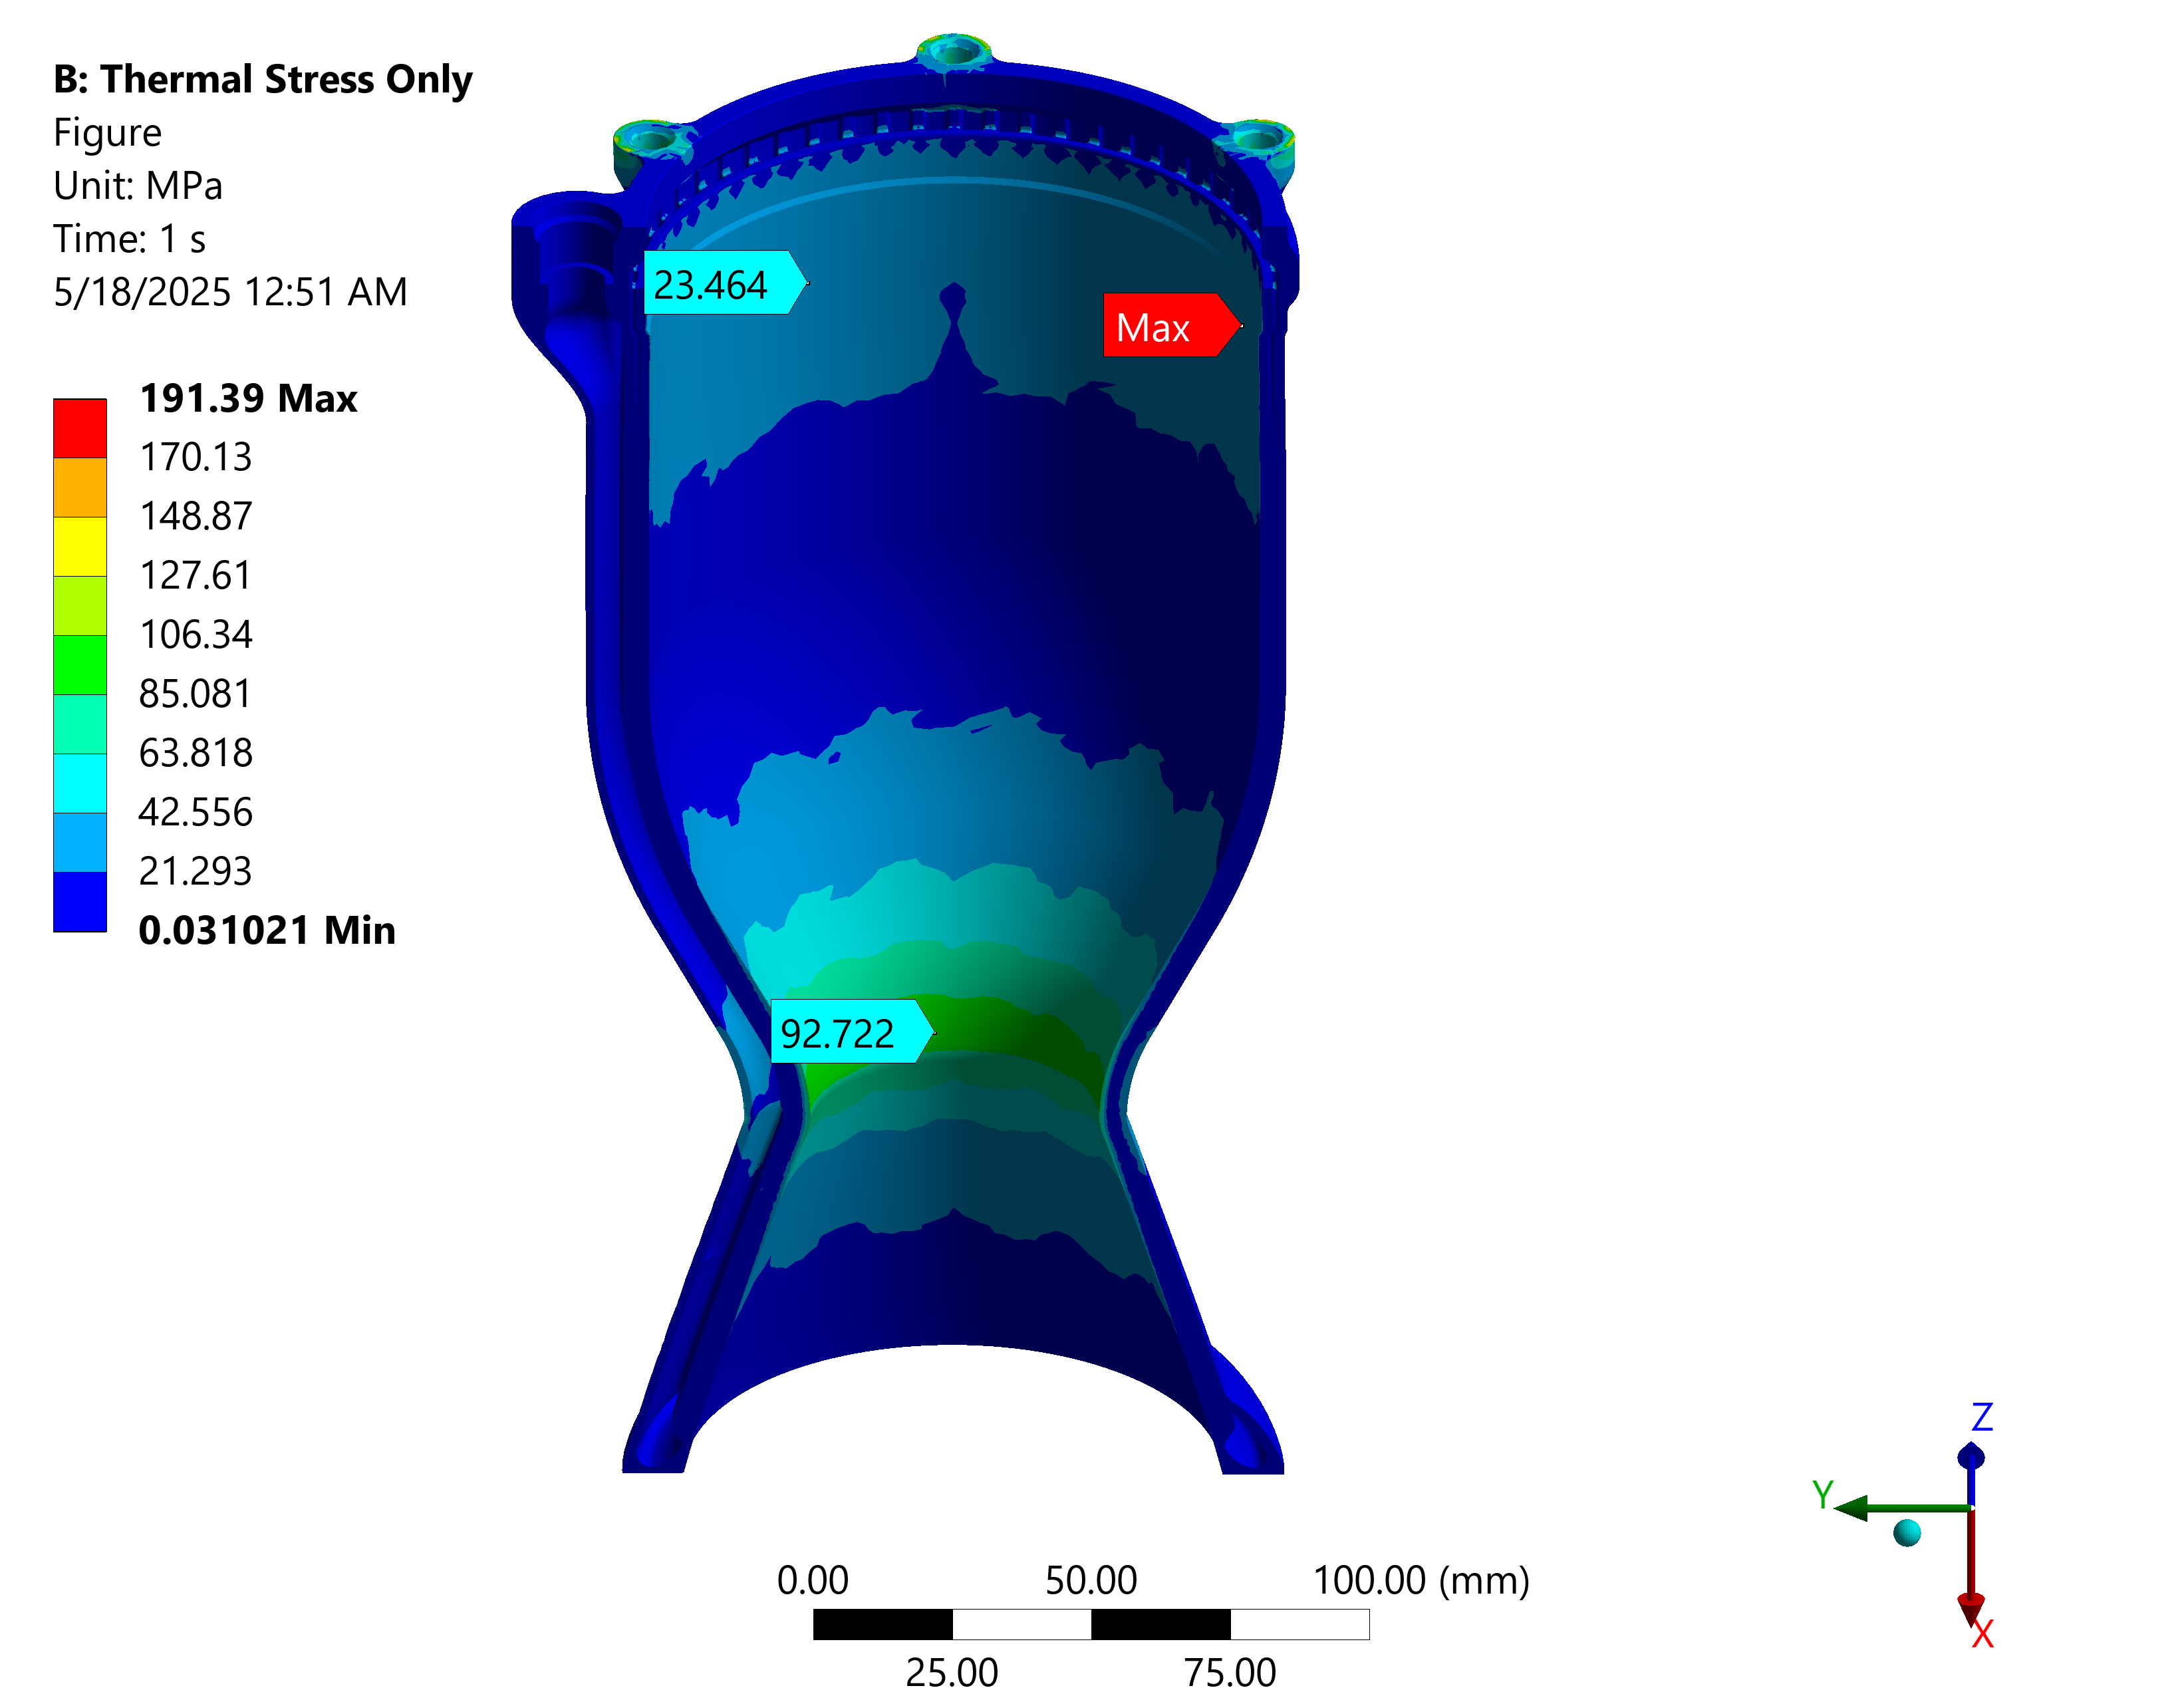
\includegraphics[width=1\linewidth]{Images/themal_stress_only.png}
    \caption{Thermal Stress}
    \label{fig:Thermal Stress}
\end{figure}
The Thermal stress reaches a maximum of 90 MPA at the throat. This is expected due to the thermal gradient being the greatest at this area. 
\begin{figure}
    \centering
    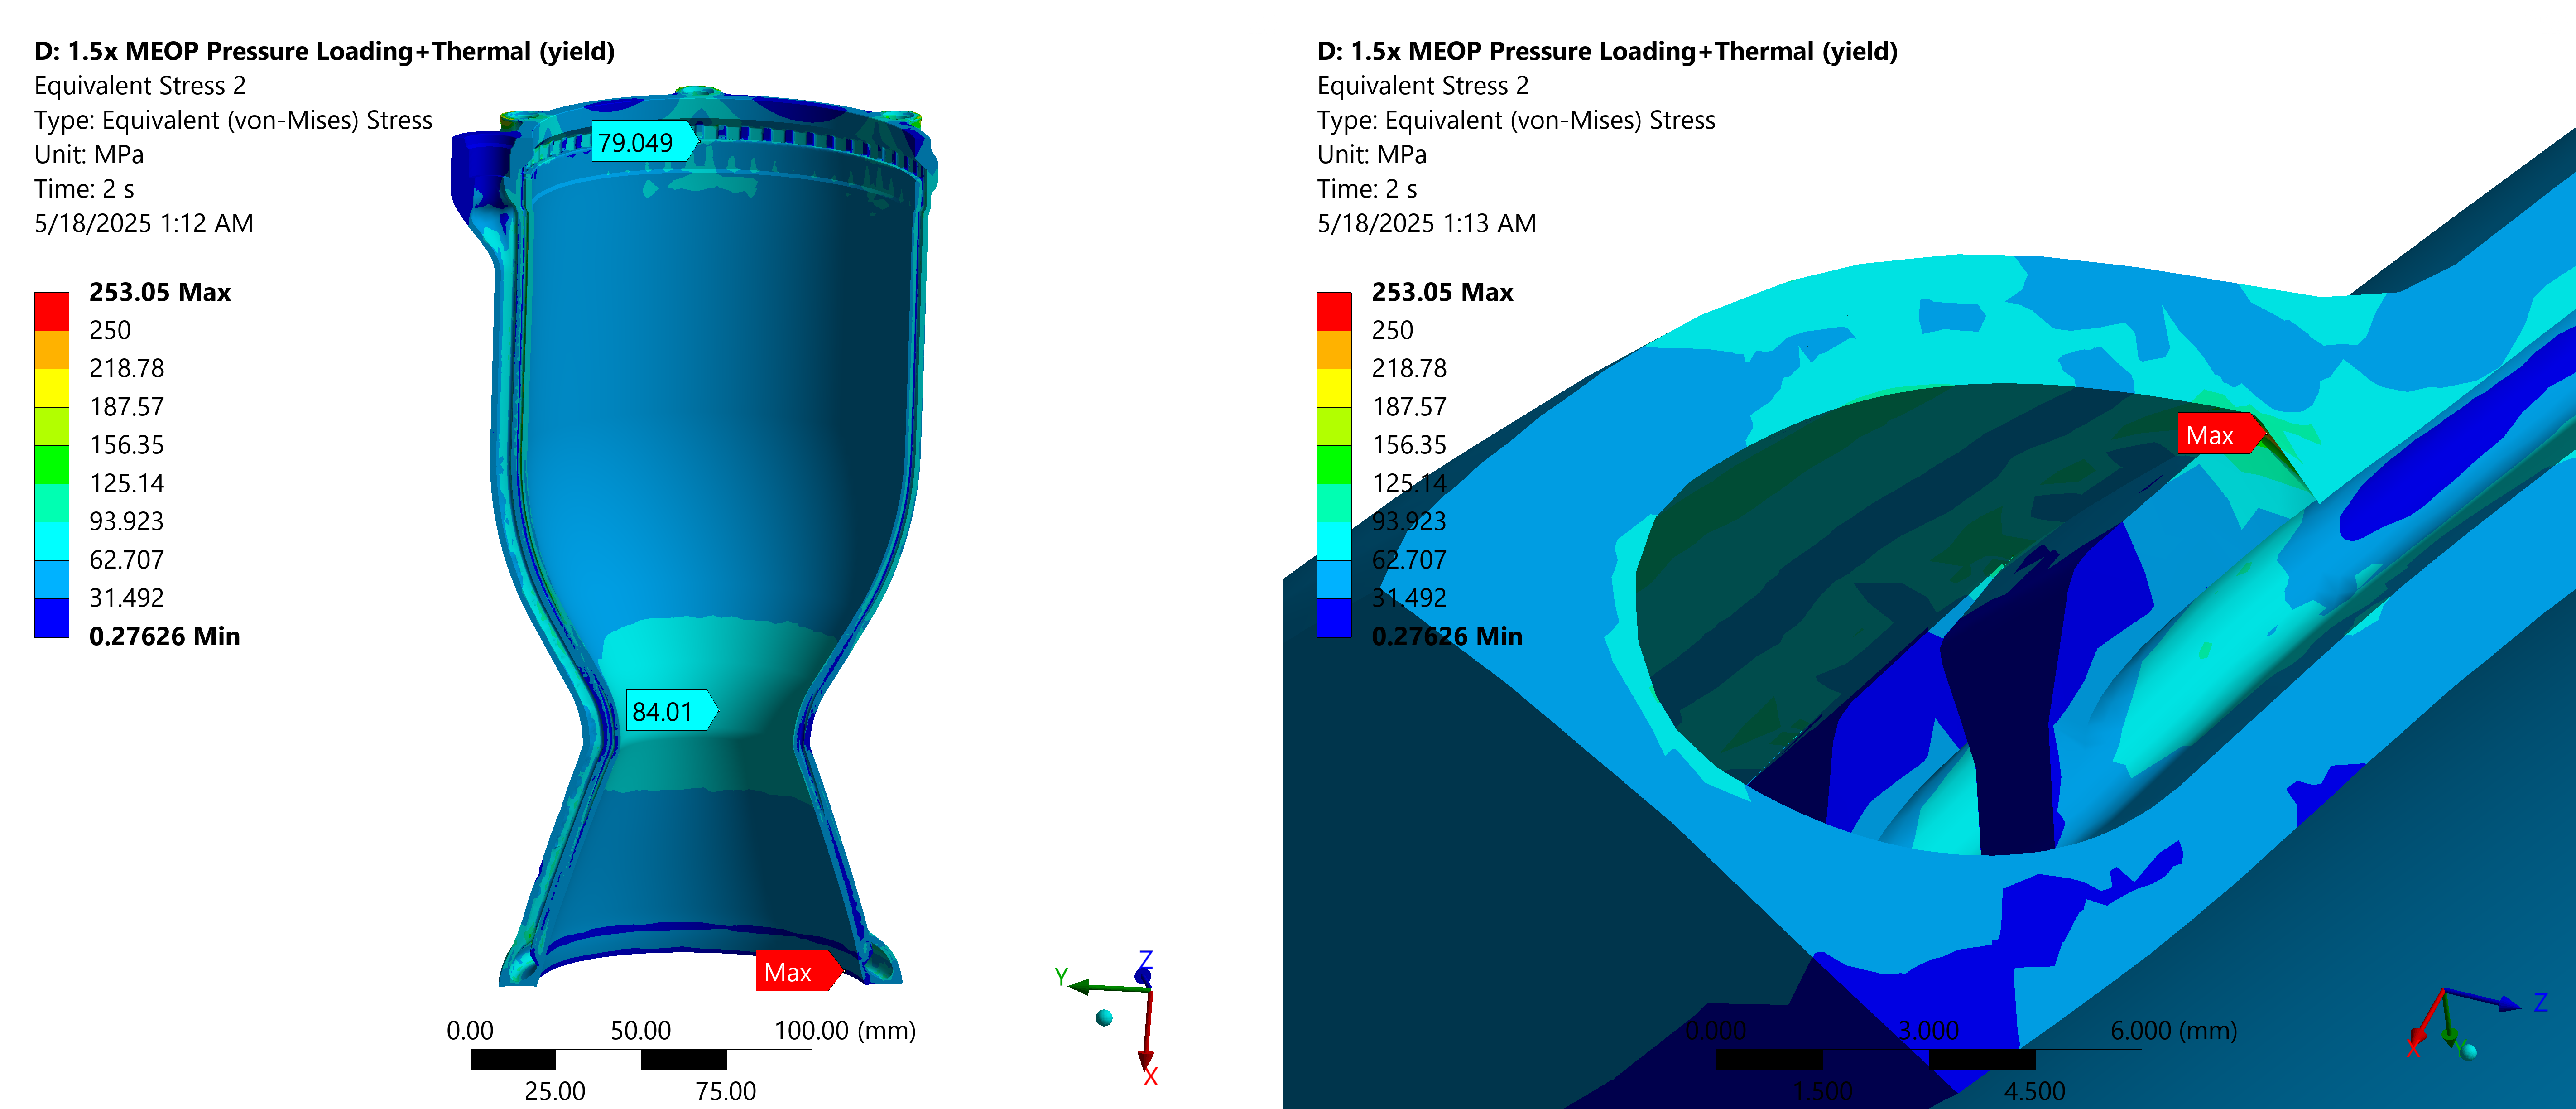
\includegraphics[width=1\linewidth]{Images/Yield Pressure and Thermal Loading.png}
    \caption{Enter Caption}
    \label{fig:Yield Pressure and Thermal Loading}
\end{figure}
The results for 1.5x MEOP show that the Von Mises stress does not exceed 253 MPA. The peak stress is observed at the edge of the cooling channel, which is not entirely unexpected. The feature is small, and has sharp edges. Any yielding in this area would be non-detrimental. 
\begin{figure}
    \centering
    \includegraphics[width=1\linewidth]{Images/Yield Pressure Loading Only.png}
    \caption{Yield Pressure Only}
    \label{fig:Yield Pressure Only}
\end{figure}
There is also high stress near the bolt interfaces, however this is also expected. Again, there is a sharp chamfer which is a stress concentration. This is not a concern as the preload will be less in the actual build, which will reduce this stress. Local yielding is also non detrimental in this area. 
The results for 1.5x MEOP combined with thermal loading show an indentical peak stress, but higher mean stress, especially in the chamber. This is acceptable. 

\begin{figure}
    \centering
    \includegraphics[width=1\linewidth]{Images/Ultimate Pressure and Thermal loading.png}
    \caption{Ultimate Pressure and Thermal loading}
    \label{fig:Ultimate Pressure and Thermal loading}
\end{figure}
Stress does not exceed the Ultimate Tensile Strength at any location in this result. 
\begin{figure}
    \centering
    \includegraphics[width=1\linewidth]{Images/Combined Mesh.png}
    \caption{Combined Mesh}
    \label{fig:Combined Mesh}
\end{figure}
\begin{figure}
    \centering
    \includegraphics[width=1\linewidth]{Images/Combined Mesh Quality.png}
    \caption{Combined Mesh Quality}
    \label{fig:Combined Mesh Quality}
\end{figure}
Above is shown the mesh used in the combined analysis modules.  This mesh is comprised of 1.6 million elements. Mesh quality is acceptable, but there are many elements with a high aspect ratio. This will reduce accuracy especially in areas of high stress. 

A higher mesh fidelity was desired on the top of the combustion chamber, so a breakout model was used there to allow for more elements on the through thickness without exceeding the solve capabilities of the Swanson machines.  A nonlinear adaptive method was attempted to increase mesh fidelity where strain energy exceeded a set criterion. This method is promising because it can theoretically reduce the burden of analysis preparation of breakout models by only refining the mesh in areas that are under stress. In this way, the manual labor required to prepare the ANSYS model is much less, so any design changes can be quickly re-analyzed. No breakout models would be needed, because the element count would be low enough to be solved directly. This method did not initially work on the combined chamber, so I made a breakout model to refine the parameters. This breakout model is a bolted joint under preload and pressure. It functioned exactly as expected. Again, This method was attempted on the full chamber, but because of the geometrical complexity of the engine chamber, the solver rejected this method for unknown reasons. Because there was no diagnostic path to follow, the method was deemed fruitless at this point in time. The nonlinear adaptive region is a new feature that seems to be very promising, but not quite fully developed. 

\subsection{Sectioned Breakout Model
}
A breakout model was made of the top of the combustion chamber combined with the injector to more accurately analyze the stress in this area. Because the model is smaller, a finer mesh can be used without an unreasonable number of elements. 
\begin{figure}
    \centering
    \includegraphics[width=1\linewidth]{Images/Breakout Model Mesh.png}
    \caption{Breakout Model Mesh}
    \label{fig:Breakout Model Mesh}
\end{figure}
\begin{figure}
    \centering
    \includegraphics[width=1\linewidth]{Images/Breakout Mesh-Chamber and Bolts Cross Section.png}
    \caption{Breakout Mesh-Chamber and Bolts Cross Section}
    \label{fig:Breakout Mesh-Chamber and Bolts Cross Section}
\end{figure}
\begin{figure}
    \centering
    \includegraphics[width=1\linewidth]{Images/Breakout Mesh Through Thickness.png}
    \caption{Breakout Mesh Through Thickness}
    \label{fig:Breakout Mesh Through Thickness}
\end{figure}
 \begin{figure}
     \centering
     \includegraphics[width=1\linewidth]{Breakout Mesh Quality.png}
     \caption{Breakout Mesh Quality}
     \label{fig:Breakout Mesh Quality}
 \end{figure}
 The breakout mesh is comprised of 1.5 million elements, which is comparable to the combined model, however the element size is much smaller,  at 0.8mm. This also allowed the element quality to increase significantly, all without increasing computation time. Additionally, two through thickness elements are now present in all areas, greatly increasing the accuracy of stress results due to pressure loading. Thermal loading is not considered in this area because there is no temperature data for the injector.
\begin{figure}
    \centering
    \includegraphics[width=1\linewidth]{Images/1.5x MEOP Pressure Load Combined.png}
    \caption{1.5x MEOP Pressure Load Combined}
    \label{fig:1.5x MEOP Pressure Load Combined}
\end{figure}
 \begin{figure}
     \centering
     \includegraphics[width=1\linewidth]{Images/1.5X MEOP Cross Section.png}
     \caption{1.5X MEOP Cross Section}
     \label{fig:1.5X MEOP Cross Section}
 \end{figure}
\begin{figure}
    \centering
    \includegraphics[width=1\linewidth]{Images/Yield High Stress Locations.png}
    \caption{Yield High Stress Locations}
    \label{fig:Yield High Stress Locations}
\end{figure}
There is an area of high stress on the inner wall of the fuel channel by the fuel inlet port. This area of high stress may exist along the whole length of the fuel transfer tube 

This area of high stress is less pronounced on the full ANSYS model. On the breakout model, these areas of particularly high stress are within 2mm of the boundary, which may be contributing to this effect. Because the boundary is frictionless, the wall only has two degrees of freedom, moving outward, or rotating. As the walls are forced outward by the pressure, a local bending moment is created on the inside of the channel.
\begin{figure}
    \centering
    \includegraphics[width=1\linewidth]{Images/High Stress Areas Combined Model.png}
    \caption{High Stress Areas Combined Model}
    \label{fig:High Stress Areas Combined Model}
\end{figure}
This same area on the full model does not have the same high stress locations. This may be in part due to a less refined mesh, however it is more likely that the boundary condition in the sliced model caused this high stress area. 

\begin{figure}
    \centering
    \includegraphics[width=1\linewidth]{Sliced Chamber Yield Results.png}
    \caption{Sliced Chamber Yield Results}
    \label{fig:Sliced Chamber Yield Results}
\end{figure}
The other high stress area is right around the bolts, which is expected and does not exceed ULT, or exceed maximum strain values. 
\begin{figure}
    \centering
    \includegraphics[width=1\linewidth]{Images/2x MEOP Ultimate Load Sliced Model.png}
    \caption{2x MEOP Ultimate Load Sliced Model}
    \label{fig:2x MEOP Ultimate Load Sliced Model}
\end{figure}

 \begin{figure}
     \centering
     \includegraphics[width=1\linewidth]{2x MEOP Ultimate Cross Section.png}
     \caption{2x MEOP Ultimate Cross Section}
     \label{fig:2x MEOP Ultimate Cross Section}
 \end{figure}
 \begin{figure}
     \centering
     \includegraphics[width=1\linewidth]{Images/2x MEOP Ultimate Chamber.png}
     \caption{2x MEOP Ultimate Chamber}
     \label{fig:2x MEOP Ultimate Chamber}
 \end{figure}
 \begin{figure}
     \centering
     \includegraphics[width=1\linewidth]{Images/2x MEOP Ultimate Strain.png}
     \caption{2x MEOP Ultimate Strain}
     \label{fig:2x MEOP Ultimate Strain}
 \end{figure}
 Strain reaches a maximum of 0.39\% which is far below the fracture strain of 9\% 
\begin{figure}
    \centering
    \includegraphics[width=1\linewidth]{Images/Chamber Directional Deformation.png}
    \caption{Chamber Directional Deformation}
    \label{fig:Chamber Directional Deformation}
\end{figure}
In the 1.5x load factor  results, the directional deformation in the radial direction reaches a maximum of 0.0031". This clearance should be considered with the existing O ring clearance to ensure that it does not exceed acceptable values and cause an O ring failure. 
\begin{figure}
    \centering
    \includegraphics[width=1\linewidth]{Images/Limits For Extrusion.png}
    \caption{Limits For Extrusion}
    \label{fig:Limits For Extrusion}
\end{figure}

 According to the Parker O-ring handbook, approximately $0.012''$ of diametral clearance is acceptable at 1000 PSI. The design provides a nominal diametral clearance of $0.003$-$0.006$ inches, which combined with the maximum calculated deformation of $0.003$ inches results in a maximum diametral clearance of $0.009$ inches during operation. This remains within acceptable limits to maintain proper sealing.

The O-rings will only be in contact with fuel and combustion chamber gases so fluorosilicone O rings are not needed. These O rings will be exposed to combustion chamber temperatures, as well as combustion chamber gases and unburnt fuel and oxidizer.  The safest option would be to choose Kalrez  or Viton O rings. Viton o rings will be much less expensive, and can withstand up to 500K.  

\subsection{Injector Analysis
}
 The injector was not a focus of the FEA study because the geometry is not completely finalized. However, the ANSYS results can still serve as a reference to inform future design improvements. 
 \begin{figure}
     \centering
     \includegraphics[width=1\linewidth]{Images/Injector 1.5x MEOP Pressure Loading + Thermal.png}
     \caption{Injector 1.5x MEOP Pressure Loading + Thermal}
     \label{fig:Injector 1.5x MEOP Pressure Loading + Thermal}
 \end{figure}
Apart from the stress concentrations around the film cooling holes, it appears that the injector will withstand nominal structural loading.


 
\subsection{Analysis Approach}

The implementation of the 3-2-1 method for constraints was applied, which restrains 3 points on a plane in translation to better simulate real-world mechanical constraints. This approach significantly improved the fidelity of the analysis results.

For the CFD analysis, boundary conditions were defined as:
\begin{itemize}
    \item Inlet pressure: $552,909\,\text{Pa}$
    \item Outlet pressure: $722\,\text{Pa}$
    \item Resulting pressure drop: approximately $80\,\text{PSI}$
\end{itemize}

A combined structural analysis including bolts was conducted to validate whether the observed yielding at the top of the chamber was a real phenomenon or an artifact of the simplified model. 

\subsection{Stress Analysis Results}

The von Mises stress distribution showed acceptable levels throughout the chamber body, with localized regions of high stress around bolt holes as expected. Stress in these areas remained below ultimate limits and did not indicate a risk of failure.

The elastic-plastic analysis with large deflection and nonlinear material properties showed that the structure remained intact at ultimate load with no separation of the bolted joint interface. Maximum strain reached $0.39\%$, which is significantly below the fracture strain of $9\%$ for the AlSi10Mg material.

In the 1.5x load factor analysis, the directional deformation in the radial direction reached a maximum of $0.0031$ inches. This deformation was evaluated in conjunction with the existing O-ring clearance to ensure it would not exceed acceptable values or compromise sealing performance.

According to the Parker O-ring handbook, approximately $0.012''$ of diametral clearance is acceptable for the application. The design provides a nominal diametral clearance of $0.003$-$0.006$ inches, which combined with the maximum calculated deformation of $0.003$ inches results in a maximum diametral clearance of $0.009$ inches during operation. This remains within acceptable limits to maintain proper sealing.

\section{Thermal Analysis and CFD}

\subsection{CFD Setup and Methodology}

The Computational Fluid Dynamics analysis utilized a 3D pressure-based model with SST k-omega turbulence modeling. The mesh generated for the analysis contained 9,950,025 cells with 49,014,118 faces and 32,472,736 nodes. Mesh quality metrics were monitored, with:
\begin{itemize}
    \item Minimum orthogonal quality = 0.26141
    \item Maximum aspect ratio = 88.737
\end{itemize}

Mass flow boundary conditions were implemented at both inlet and outlet, with modeled surface roughness to capture realistic flow behavior. The model geometry was prepared using watertight meshing in SolidWorks and Ansys Discovery.
\begin{figure}
    \centering
    \includegraphics[width=1\linewidth]{Images/Inlet Mesh Cross Section.png}
    \caption{Inlet Mesh Cross Section}
    \label{fig:Inlet Mesh Cross Section}
\end{figure}
\begin{figure}
    \centering
    \includegraphics[width=1\linewidth]{Images/Manifold Mesh Cross Section.png}
    \caption{Manifold Mesh Cross Section}
    \label{fig:Manifold Mesh Cross Section}
\end{figure}
\begin{figure}
    \centering
    \includegraphics[width=1\linewidth]{Images/CFD Surface Mesh.png}
    \caption{CFD Surface Mesh}
    \label{fig:CFD Surface Mesh}
\end{figure}
\begin{figure}
    \centering
    \includegraphics[width=0.5\linewidth]{Mass Flow Rate Inlet and Outlet.png}
    \caption{Mass Flow Rate Inlet and Outlet}
    \label{fig:Mass Flow Rate Inlet and Outlet}
\end{figure}
\section{CFD Results 
}
\begin{figure}
    \centering
    \includegraphics[width=1\linewidth]{Images/Coolant Velocity Streamlines.png}
    \caption{Coolant Velocity Streamlines}
    \label{fig:Coolant Velocity Streamlines}
\end{figure}

\begin{figure}
    \centering
    \includegraphics[width=1\linewidth]{RPA Coolant Velocity Graph.png}
    \caption{RPA Coolant Velocity Graph}
    \label{fig:RPA Coolant Velocity Graph}
\end{figure}

\begin{figure}
    \centering
    \includegraphics[width=1\linewidth]{Images/Single Streamline Velocity vs Axial Position.png}
    \caption{Single Streamline Velocity vs Axial Position}
    \label{fig:Single Streamline Velocity vs Axial Position}
\end{figure}
The fluent results for coolant velocity closely matches the RPA results. The discrepancy in velocity is likely due to the slightly different geometry in CAD vs the cooling channels modeled in RPA, as the RPA channels are rectangular but the CAD channels have rounded corners, slightly reducing the cross sectional area. This increases peak velocity a minor amount. A more significant effect is seen from 0-0.09m from the outlet, where the coolant velocity is around 0.9m/s less than in RPA on average. This will increase the temperature of this region, as the heat transfer coefficient is heavily dependent on velocity.
\begin{figure}
    \centering
    \includegraphics[width=1\linewidth]{Images/Velocity Cross Sectional Profiles.png}
    \caption{Velocity Cross Sectional Profiles}
    \label{fig:Velocity Cross Sectional Profiles}
\end{figure}
A cross section was taken at the throat and at the middle of the combustion chamber. The throat experiences extremely high heat flux, so it is critical that the coolant is traveling at the correct velocity and that the coolant is uniformly distributed around the chamber. The midchamber cross section is analyzed to determine the average coolant velocity, because the single streamline plot is not accurate enough to conclude whether the coolant is matching the RPA simulated values. 

\begin{figure}
    \centering
    \includegraphics[width=1\linewidth]{Throat Velocity Profiles.png}
    \caption{Throat Velocity Profiles}
    \label{fig:Throat Velocity Profiles}
\end{figure}
\begin{figure}
    \centering
    \includegraphics[width=1\linewidth]{Images/Throat Velocity Inlet Side.png}
    \caption{Throat Velocity Inlet Side}
    \label{fig:Throat Velocity Inlet Side}
\end{figure}

\begin{figure}
    \centering
    \includegraphics[width=1\linewidth]{Midchamber Velocity.png}
    \caption{Midchamber Velocity}
    \label{fig:Midchamber Velocity}
\end{figure}
\begin{figure}
    \centering
    \includegraphics[width=1\linewidth]{Midchamber Velocity Far From Inlet.png}
    \caption{Midchamber Velocity Far From Inlet}
    \label{fig:Midchamber Velocity Far From Inlet}
\end{figure}
\begin{figure}
    \centering
    \includegraphics[width=1\linewidth]{Images/Midchamber Velocity Close to Inlet.png}
    \caption{Midchamber Velocity Close to Inlet}
    \label{fig:Midchamber Velocity Close to Inlet}
\end{figure}

The coolant is traveling significantly faster through the channels which are at a similar clocking to the fuel inlet channel. This is not unexpected, as the pressure is highest at the base of the fuel inlet. Although there is an imbalance in fuel velocity, the average velocity is still in line with the RPA simulations which suggests that this mismatch is acceptable. The fuel imbalance could be remedied by changing the cross section of the bottom coolant distribution manifold such that the coolant is always traveling at the same velocity regardless of distance from the fuel inlet. 

\subsection{Pressure Loss Results}
The pressure loss across the fuel flow path was measured by taking the difference in pressure between the inlet and outlet. The resulting pressure drop is approximately 80 PSI.
Inlet pressure: 552909 pa 
Outlet pressure: 722 pa
Pressure drop= \~80 PSI 

The pressure loss calculated by hand was 24.76 PSI, which is around a third of what was calculated in FLUENT. The pressure loss calculated by RPA was 6.15 PSI. 

 

\section{Material Properties and Considerations}

\subsection{AlSi10Mg Properties}

The analysis utilized AlSi10Mg aluminum alloy material properties, with particular attention to temperature-dependent characteristics. The material exhibits significant variation in mechanical properties at elevated temperatures:

\begin{table}[htbp]
    \centering
    \caption{Temperature-dependent mechanical properties of AM-SLM AlSi10Mg specimens}
    \begin{tabular}{ccccc}
        \hline
        Temperature & Elastic Modulus & Yield Stress & Ultimate Tensile & Elongation at \\
        ($^{\circ}$C) & ($E$, GPa) & (YS, MPa) & Stress (UTS, MPa) & fracture ($\varepsilon_f$, \%) \\
        \hline
        25 & 77.6 & 204 & 358 & 7.2 \\
        50 & 75.5 & 198 & 341 & 8.5 \\
        100 & 72.8 & 181 & 286 & 10.0 \\
        150 & * & 182 & 241 & 14.7 \\
        200 & * & 158 & 189 & 16.4 \\
        250 & * & 132 & 149 & 30.9 \\
        300 & * & 70 & 73 & 41.4 \\
        350 & * & 30 & 33 & 53.8 \\
        400 & * & 12 & 14 & 57.4 \\
        \hline
    \end{tabular}
    \label{tab:alsi10mg_properties}
    \\ \small{* Young's modulus cannot be determined accurately above $100^{\circ}$C.}
\end{table}

Different values of yield strength (YS) and ultimate tensile strength (UTS) are reported by various manufacturers. The analyzed sample had been stress relieved, resulting in relatively lower strength values compared to other processing conditions. 

According to XMake (the manufacturing partner), their as-built AlSi10Mg has the following properties:

\begin{itemize}
    \item Tensile strength (horizontal direction): $430 \pm 20\,\text{MPa}$
    \item Yield strength: $245 \pm 10\,\text{MPa}$
    \item Elastic modulus: $70 \pm 5\,\text{GPa}$
    \item Elongation: $9 \pm 2\%$
    \item Hardness: $120 \pm 5\,\text{HV}$
    \item Long-term operating temperature: Below $250^{\circ}\text{C}$
\end{itemize}


XMake did not provide yield strength vs temperature, however the ANSYS AlSi10Mg material card has a similar yield strength at room temperature. Therefore, it can be assumed that the ANSYS material will perform similarly to how the Xmake material will under higher temperatures. The ANSYS data is used for all yield safety margin calculations in this report.  
\begin{figure}
    \centering
    \includegraphics[width=1\linewidth]{Images/AlSi10Mg Yield Strength vs Temperature GRANTA.png}
    \caption{AlSi10Mg Yield Strength vs Temperature GRANTA}
    \label{fig:AlSi10Mg Yield Strength vs Temperature GRANTA}
\end{figure}

\subsection{Thermal Conductivity Considerations}

Thermal conductivity was modeled as $110\,\text{W/m}\cdot\text{K}$ for the analysis. Research indicates that heat treatment can significantly improve the thermal performance of AlSi10Mg \cite{martinez2020}:

\begin{itemize}
    \item Post-manufacture annealing eliminates thermal conductivity anisotropy present in the as-built condition
    \item Annealing enhances conductivity by approximately $30\%$ in the transverse direction
    \item Solution heat treatment increases thermal conductivity by $36\%$ compared to as-built
    \item T6-like treatment provides the greatest improvement ($44\%$ over as-built) \cite{martinez2020}
\end{itemize}

\begin{figure}
    \centering
    \includegraphics[width=1\linewidth]{Images/Thermal Conductivity vs Temperature.png}
    \caption{Thermal Conductivity vs Temperature \cite{martinez2020}}
    \label{fig:Thermal Conductivity vs Temperature}
\end{figure}

If the printed component were heat treated to bring thermal conductivity closer to $140\,\text{W/m}\cdot\text{K}$, peak temperatures would be reduced by approximately $10\,\text{K}$ to $455\,\text{K}$. This improvement is related to the evolution of the AlSi10Mg microstructure, particularly the breakdown of the Si cellular structure.
The EOS T6 temper appears to be the optimal heat treatment for more uniform material properties.

According to XMake (the manufacturing partner), their as-built AlSi10Mg has the following properties:

\begin{itemize}
    \item Tensile strength (horizontal direction): $430 \pm 20\,\text{MPa}$
    \item Yield strength: $245 \pm 10\,\text{MPa}$
    \item Elastic modulus: $70 \pm 5\,\text{GPa}$
    \item Elongation: $9 \pm 2\%$
    \item Hardness: $120 \pm 5\,\text{HV}$
    \item Long-term operating temperature: Below $250^{\circ}\text{C}$
\end{itemize}

\section{Manufacturing Process}

The engine will be printed nozzle side down using a Han metal 3D printer. Critical features such as the injector interface bore on the chamber will require post-machining according to the detailed engineering drawings per \hyperref[doc:chamberPost]{Appendix~\ref*{app:supportDocs}, 
“Liquid-Engine Chamber Post-Processing Report”}.  To achieve the correct dimensions after machining, the 3D printed model was modified to incorporate additional material around the bore.

The manufacturing model also has the bolt holes removed, as these will be drilled and tapped during the post-machining process. This approach ensures proper thread engagement and dimensional accuracy for critical fastening features. 

As of 5/18/25 the engine has been 3D printed, and is now undergoing post process machining at XMAKE in China.



\section{Future Work}
\begin{itemize}
  \item \textbf{Additional Computational Fluid Dynamics (CFD) and flow-path optimization:}
        perform CFD simulations on the internal flow path through the injector body.
  \item \textbf{Injector design optimization:}
        improve the pintle injector to enhance fuel–oxidizer mixing and investigate optimal momentum ratios; explore methodologies for independent throttling of fuel and oxidizer while maintaining stable combustion.
  \item \textbf{Throttle-control investigation:}
        investigate mechanical and flow-based solutions to independently throttle fuel and oxidizer, enabling dynamic thrust modulation; evaluate thermal-management strategies under varying throttle conditions to prevent overheating at low power levels.
  \item \textbf{Instrumentation integration:}
        evaluate the integration of thermocouples and pressure transducers for real-time chamber-condition monitoring.
  \item \textbf{Manufacturing validation:}
        inspect the combustion chamber through dimensional measurements; send the injector body to Xmake for manufacturing.
\end{itemize}



